\documentclass[a4paper,11.5pt]{report}


\usepackage[T1]{fontenc} % Westeuropäische Codierung
\usepackage[utf8]{inputenc} % Umlaute
\usepackage{textcomp} % Verschiedene Textsymbole
\usepackage[ngerman]{babel} % Sprache des Dokuments. Beeinflusst Überschriften, Datumsformat, etc.
\usepackage[pdftex]{graphicx} % Bilder einbinden
\usepackage[table]{xcolor} % Eigene Farben definieren
\usepackage{fancyhdr} % Anpassbare Header und Footer
\usepackage[babel,german=quotes]{csquotes}
\usepackage{geometry} % Zum Anpassen der Seitenränder
\usepackage{blindtext} % Zum Erzeugen von Blindtext
\usepackage{setspace} % Um die Abstände von Überschriften zum Text anzupassen
\usepackage{libertine} % fancy Schriftart, die small capitals unterstützt
% \usepackage{helvet}
\usepackage{hyperref} % Verlinkungen und PDF Optionen
\usepackage{titlesec} % Überschriftenformat anpassen
\usepackage{booktabs} % rules für Tabellen
\usepackage[printonlyused]{acronym} % Abkürzungen, es werden nur die angezeigt, die benutzt werden
\usepackage{tabularx} % Tabellen über die gesamte Breite
\usepackage{caption} % Zur Anpassung von Titeln von Gleitobjekten
\usepackage{diagbox} % Überschrift mit Schrägstrich in Tabellenkopfzeile
\usepackage{float} % Einige Zusatzoptionen für float Objekte
\usepackage[backend=biber, style=authoryear-icomp, mergedate=false, dashed=false, maxbibnames=99]{biblatex} % Bibliografie, möglichst alle Autoren anzeigen
\usepackage[babel,german=quotes]{csquotes} % Zitationsoptionen
\let\counterwithout\relax
\let\counterwithin\relax
\usepackage{chngcntr}  % für fortlaufende Fußnotennummerierung
\usepackage[colorinlistoftodos]{todonotes} % ToDos
\usepackage{moreverb} % Datei Ein- und Ausgabe
\usepackage{listings} % Listings
\usepackage{blindtext}
\usepackage[normalem]{ulem} % Strike Through Text
\usepackage{rotating}
\usepackage{multirow}
\usepackage{appendix}
\usepackage[bottom]{footmisc}

\def\semester{7}
\def\modul{asdf}
\def\titel{Evaluierung des Einsatzes von ChatOps zur Arbeitserleichterung der Mitarbeiter im Rechenzentrum beim Umgang mit einer Configuration--Management--Database}
\def\autor{asdf}
\def\studiengang{Wirtschaftsinformatik}
\def\ort{Köln}
% \def\Abgabedatum{\today}
\def\Abgabedatum{4. Juli 2019}
\def\betreuer{Stiven \textsc{Raso} M.A.}

% Sollte noch überarbeitet werden
\def\autorkurz{ Weiss}
\def\autorlang{ Kevin Weiss}
\def\autor{Kevin \textsc{Weiss}   \\   Matrikel-Nr. 415171}

\newcommand*{\quelle}{%
  ~\\\smallskip\footnotesize Quelle: \cite
%  \footnotesize Quelle: \cite
%  \footcites
}

\newcommand*{\quelleeigen}{%
  ~\\\smallskip\footnotesize Quelle: Eigene Abbildung nach: \cites
%  \footnotesize Quelle: Eigene Abbildung nach: \cites
%  \footnotesize (Quelle: Eigene Abbildung nach: \cite[#1]{#2})
}

\newcommand*{\eigen}{%
  ~\\\smallskip\footnotesize Quelle: Eigene Darstellung
  %\footnotesize Quelle: Eigene Darstellung
}




\newcommand{\HRule}{\rule{\linewidth}{0.5mm}} %Für Titelseite
\newcommand{\hsp}{\hspace{20pt}} %Für Chapter Überschriften
\newcommand{\note}[2][]{\todo[color={red!100!green!33}, #1]{#2}}
\newcommand{\question}[2][]{\todo[color=green, #1]{#2}}
\newcommand{\dotoday}[2][]{\todo[color=red, #1]{#2}}
\newcommand{\todoin}[2][]{\todo[inline, #1] {#2}}
\newcommand{\nicetohave}[2][]{\todo[color=blue!30, #1]{#2}}

% \presetkeys%
%     {todonotes}%
%     {inline}{}
%

\immediate\write18{texcount -inc -incbib -sum -total -nosub 01_Einleitung.tex 02_Grundlagen.tex 03_Hauptkapitel.tex 04_Betriebswirtschaftliche_Betrachtung.tex 05_Fazit.tex > /tmp/wordcount.tex}
\newcommand\wordcount{
\verbatiminput{/tmp/wordcount.tex}}

\definecolor{gray75}{gray}{0.75}
\definecolor{fom}{HTML}{23a092}
% \font\myfont=libertine at 12pt
% \definefont[myfont][name:libertine at 12pt]

\renewcommand*\familydefault{\sfdefault}
% \renewcommand*\familydefault{\rmdefault}
\newcommand{\mynormal}{\fontsize{12}{12}\selectfont}
\newcommand{\mylarge}{\fontsize{14}{14}\selectfont}
\newcommand{\MyLarge}{\fontsize{17}{17}\selectfont}
\newcommand{\MYLARGE}{\fontsize{20}{20}\selectfont}

\newcommand{\fomhead}{
	\fancyhead{}
	\fancyfoot{} %alle Kopf- und Fußzeilenfelder bereinigen
	\fancyhead[R]{\mynormal Seite \thepage}
  \fancyhead[L]{
\includegraphics[width=1cm]{Anhang/fom.jpg}}

	\renewcommand{\headrulewidth}{0.2pt} %obere Trennlinie
%	\fancyfoot[L]{\mynormal\autorkurz}
	\fancyfoot[L]{}
	\fancyfoot[C]{}
	\fancyfoot[R]{}
%	\renewcommand{\footrulewidth}{0.2pt} %untere Trennlinie
	\patchcmd{\headrule}{\hrule}{\color{gray75}\hrule}{}{}
%	\patchcmd{\footrule}{\hrule}{\color{gray75}\hrule}{}{}
}

\fancypagestyle{plain}{\fomhead}% Für Kapitelseiten, Inhaltsverzeichnis, etc nutzen
\fomhead% Für "`normale"' Seiten setzen

\setlength{\headheight}{33pt}
\onehalfspacing

% \geometry{a4paper,left=3.4cm,right=3.4cm, top=3cm, bottom=3cm}
\geometry{a4paper,left=3cm,right=3cm, top=3cm, bottom=3cm}

\titleformat{\chapter}[display] {\normalfont\huge\bfseries}{\textcolor{fom}{\chaptertitlename\ \thechapter}}{20pt}{\Huge\textcolor{fom}}
% \titleformat{\chapter}[hang]{\vspace{5ex} \LARGE\bfseries\scshape}{\textcolor{fom}{Kapitel \thechapter}\hsp}{20pt}{\LARGE\bfseries\textcolor{fom}}
% \titleformat{\chapter}[hang]{\vspace{5ex} \LARGE\bfseries\scshape}{\textcolor{fom}\thechapter\hsp\textcolor{gray75}{|}\hsp}{20pt}{\LARGE\bfseries\textcolor{fom}}
% \titleformat{\chapter}[display] {\normalfont\huge\bfseries}{\chaptertitlename\ \thechapter}{20pt}{\Huge}  % Default Titleformat

% \titlespacing{\chapter}{0mm}{-4em}{2.0em}
% \titlespacing{\section}{0mm}{-0.5em}{-0.3em}
% \titlespacing{\subsection}{0mm}{-0.5em}{-0.3em}
% \titlespacing{\subsubsection}{0mm}{-0.5em}{-0.3em}

\setlength{\parskip}{0.5em} % 1ex plus 0.5ex minus 0.2ex}
\setlength{\parindent}{0.5em}
\setlength\bibitemsep{\baselineskip}
% \setlength{\arrayrulewidth}{0.7mm}
\setlength{\tabcolsep}{3pt}

% \renewcommand{\arraystretch}{1.}
\def\arraystretch{1.5}%  1 is the default, change whatever you need
\emergencystretch 3em %reduce overhanging words
\renewcommand{\labelitemi}{{\color{fom}\textbullet}}

\counterwithout*{footnote}{chapter} %Fortlaufende Nummerierung für Fußnoten
\setcounter{secnumdepth}{5} % seting level of numbering (default for "report" is 3). With ''-1'' you have non number also for chapter

\AtEndDocument{\thispagestyle{empty}} %Letzte Seite ohne Header und Footer

% \lstset{
%          basicstyle=\footnotesize\ttfamily, % Standardschrift
%          numbers=left,               % Ort der Zeilennummern
%          numberstyle=\tiny,          % Stil der Zeilennummern
%          %stepnumber=2,               % Abstand zwischen den Zeilennummern
%          numbersep=5pt,              % Abstand der Nummern zum Text
%          tabsize=2,                  % Groesse von Tabs
%          extendedchars=true,         %
%          breaklines=true,            % Zeilen werden Umgebrochen
%          keywordstyle=\color{red},
%             frame=b,
%  %        keywordstyle=[1]\textbf,    % Stil der Keywords
%  %        keywordstyle=[2]\textbf,    %
%  %        keywordstyle=[3]\textbf,    %
%  %        keywordstyle=[4]\textbf,   \sqrt{\sqrt{}} %
%          stringstyle=\color{white}\ttfamily, % Farbe der String
%          showspaces=false,           % Leerzeichen anzeigen ?
%          showtabs=false,             % Tabs anzeigen ?
%          xleftmargin=17pt,
%          framexleftmargin=17pt,
%          framexrightmargin=5pt,
%          framexbottommargin=4pt,
%          %backgroundcolor=\color{lightgray},
%          showstringspaces=false      % Leerzeichen in Strings anzeigen ?
%  }
%  \lstloadlanguages{% Check Dokumentation for further languages ...
%          %[Visual]Basic
%          %Pascal
%          %C
%          %C++
%          %XML
%          %HTML
%          python
% 				%  json
%         %  Java
%  }

\lstset{
  basicstyle=\ttfamily,
  numbers=left,               % Ort der Zeilennummern
  columns=fullflexible,
  frame=single,
  breaklines=true,
  postbreak=\mbox{\textcolor{red}{$\hookrightarrow$}\space},
}

%\DeclareCaptionFont{white}{\color{white}}
%\DeclareCaptionFormat{listing}{\colorbox{gray}{\parbox{\textwidth}{#1#2#3}}}
%\captionsetup[lstlisting]{format=listing,labelfont=white,textfont=white}
%\renewcommand\lstlistlistingname{Listings}

\newcolumntype{Y}{>{\centering\arraybackslash}X}
\newcommand\RotText[1]{\rotatebox{90}{\parbox{3.5cm}{\centering#1}}}

\renewcommand{\appendixtocname}{Anhang}

\addbibresource{Bib/Facharbeit.bib}
\addbibresource{Bib/Experteninterview.bib}
\addbibresource{Bib/Requirements.bib}
\addbibresource{Bib/CMDB.bib}
\addbibresource{Bib/Chat.bib}

%in Fusszitaten Jahre in Klammern, alte Umsetzung
%\renewbibmacro*{cite:labelyear+extrayear}{%
%\iffieldundef{labelyear}
%{}
%{\printtext[bibhyperref]{%
%\mkbibparens{%
%\printfield{labelyear}%
%\printfield{extrayear}}}}}

%\renewbibmacro*{cite}{%
%  \iffieldundef{shorthand}
%    {\ifthenelse{\ifnameundef{labelname}\OR\iffieldundef{labelyear}}
%       {\usebibmacro{cite:label}%
%        \setunit{\addspace}}
%       {\printnames{labelname}%
%        \setunit{\nameyeardelim}}%
%     \printtext[parens]{\usebibmacro{cite:labelyear+extrayear}}}% ADDED
%    {\usebibmacro{cite:shorthand}}}


%break long bib urls
\setcounter{biburllcpenalty}{7000}
\setcounter{biburlucpenalty}{8000}

%in Fusszitaten Jahre in Klammern
\makeatletter
\renewbibmacro*{cite}{%
  \iffieldundef{shorthand}
    {\ifthenelse{\ifciteibid\AND\NOT\iffirstonpage}
       {\usebibmacro{cite:ibid}}
       {\ifboolexpr{test {\ifnameundef{labelname}}
                    or test {\iffieldundef{labelyear}}}
          {\usebibmacro{cite:label}%
           \setunit{%
             \global\booltrue{cbx:parens}%
             \printdelim{nonameyeardelim}%
             \bibopenparen}%
           \usebibmacro{cite:labeldate+extradate}%
           \usebibmacro{cite:reinit}}
          {\iffieldequals{namehash}{\cbx@lasthash}
             {\ifboolexpr{test {\iffieldequals{labelyear}{\cbx@lastyear}}
                          and (test {\ifnumequal{\value{multicitecount}}{0}}
                               or test {\iffieldundef{postnote}})}
                {\setunit{\addcomma}%
                 \usebibmacro{cite:extradate}}
                {\setunit{\compcitedelim}%
                 \usebibmacro{cite:labeldate+extradate}%
                 \savefield{labelyear}{\cbx@lastyear}}}
             {\printnames{labelname}%
              \setunit{%
                \global\booltrue{cbx:parens}%
                \printdelim{nameyeardelim}%
                \bibopenparen}%
              \usebibmacro{cite:labeldate+extradate}%
              \savefield{namehash}{\cbx@lasthash}%
              \savefield{labelyear}{\cbx@lastyear}}}}}
    {\usebibmacro{cite:shorthand}%
     \usebibmacro{cite:reinit}}%
  \setunit{%
    \ifbool{cbx:parens}
      {\bibcloseparen
       \global\boolfalse{cbx:parens}}
      {}%
\multicitedelim}}

\renewbibmacro*{cite:postnote}{%
  \setunit{}%
  \printtext{%
    \ifbool{cbx:parens}
      {\bibcloseparen
       \global\boolfalse{cbx:parens}}
      {}}%
  \ifbool{cbx:loccit}
    {}
    {\usebibmacro{postnote}}}
\makeatother

\hypersetup{
 pdfauthor={\autorlang},
 pdftitle={\titel},
 pdfsubject=,
 pdfkeywords=,
 colorlinks,
 bookmarksopen,
 bookmarksopenlevel=1,
 bookmarksnumbered,
 pageanchor,
 plainpages=false,
 urlcolor=black,
 menucolor=black,
 citecolor=black,
 anchorcolor=black,
 filecolor=black,
 linkcolor=black,
 colorlinks=true
}


%addbibresource

\begin{document}
% \fontsize{10}{10}\selectfont
\begin{titlepage}
\begin{center}


\includegraphics[width=0.15\textwidth]{./Anhang/fom}~\\[1cm]

\textsc{\MYLARGE FOM Hochschule für Oekonomie \& Management}\\[0.5cm]
\textsc{\MyLarge University of Applied Sciences}\\[0.5cm]
\textsc{\MyLarge Hochschulzentrum Köln }\\[1.5cm]


\textsc{\MyLarge Bachelor-Thesis}\\[0.5cm]
\textsc{\MyLarge im Studiengang \studiengang~}\\[1.5cm]


\textsc{\MyLarge zur Erlangung des Grades eines}\\[0.5cm]
\textsc{\MyLarge Bachelor of Science (B.Sc.)}\\[0.5cm]

% Title
\HRule~\\[1cm]
{ \MYLARGE  \bfseries \titel~\\[1cm] }
\HRule~\\[1cm]



% Author and supervisor
\noindent
\begin{minipage}{0.4\textwidth}
\begin{flushleft} \mylarge
\emph{Autor:}\\
\autor~\\
%Matrikel-Nr. 415171
\end{flushleft}
\end{minipage}%
\begin{minipage}{0.4\textwidth}
\begin{flushright} \mylarge
\emph{Betreuer:} \\
\betreuer~\\~
\end{flushright}
\end{minipage}

\vfill
% Bottom of the page
%{\large \today}\\[0.5cm]
{\mylarge \ort, \Abgabedatum}\\[0.5cm]


\end{center}
\end{titlepage}
% \fontsize{14}{14}\selectfont

\pagestyle{fancy}
\pagenumbering{Roman} %Für Verzeichnisse römische Nummerierung
\setcounter{page}{2} %Seitenzähler zurücksetzen
%\newgeometry{left=4cm,right=2cm, top=4cm, bottom=2cm}
\newgeometry{left=4cm,right=2cm, top=3cm, bottom=2cm}
\reversemarginpar % todonotes auf der linken Seite

\cleardoublepage\pdfbookmark{\contentsname}{toc}\tableofcontents \newpage %Inhaltsverzeichnis
\chapter*{Abkürzungsverzeichnis}
\addcontentsline{toc}{chapter}{Abkürzungsverzeichnis}
\begin{acronym}[virtualenv]
  \acro{API}{Application Programming Interface}
  \acro{ARD}{Arbeitsgemeinschaft der öffentlich-rechtlichen Rundfunkanstalten der Bundesrepublik Deutschland}
  \acro{CAMS}{Culture of Automation, Measurement and Sharing}
  \acro{CI}{Configuration Item}
  \acrodefplural{CI}[CI's]{Configuration Items}
  \acro{CMDB}{Configuration Management DataBase}
  \acro{CMS}{Configuration Management System}
  \acro{DNS}{Domain Name System}
  \acro{DW}{Deutsche Welle}
  \acro{HiRes}{High Resolution}
  \acro{IaC}{Infrastructure as Code}
  \acro{ITIL}{IT Infrastructure Library}
  \acro{ITSM}{IT-Service-Management}
  \acro{IVZ}{Informations-Verarbeitungs-Zentrum}
  \acro{KI}{Künstliche Intelligenz}
  \acro{LAN}{Local Area Network}
  \acro{MIT}{Massachusetts Institue of Technology}
  \acro{MPC}{Music Player Client}
  \acro{MPD}{Music Player Daemon}
  \acro{rbb}{Rundfunk Berlin-Brandenburg}
  \acro{SAN}{Storage Area Network}
  \acro{SLA}{Service Level Agreement}
  \acrodefplural{SLA}[SLA's]{Service Level Agreements}
  \acro{Slack}{Searchable Log of All Conversation and Knowledge}
  \acro{SPoC}{Single Point of Contact}
  \acro{VM}{Virtuelle Maschine}
  \acro{WDR}{Westdeutscher Rundfunk}
\end{acronym}
 %Abkürzungsverzeichnis
\cleardoublepage\phantomsection\addcontentsline{toc}{chapter}{\listfigurename}\listoffigures %Abbildungsverzeichnis
\cleardoublepage\phantomsection\addcontentsline{toc}{chapter}{\listtablename}\listoftables %Tabellenverzeichnis
\cleardoublepage\phantomsection\addcontentsline{toc}{chapter}{\lstlistlistingname}\lstlistoflistings %Listings
\newpage\listoftodos\newpage
\pagenumbering{arabic} %Für Inhalt arabische Nummerierung
\setcounter{page}{1} %Seitenzähler zurücksetzen

\chapter{Einleitung}

Bereits 1966 hat Joseph Weizenbaum mit ELIZA am \acf{MIT} ein Programm geschaffen, das Strukturen in menschlicher Sprache erkennen, verstehen und auf diese antworten kann, den ersten Chatbot sozusagen.\footcite[Vgl.][o. \pno]{Weizenbaum_1966}

Auch in der heutigen Gesellschaft ist diese Funktionalität gefragter denn je. Besonders auf Unternehmenswebsiten oder Online-Shops sind immer häufiger Chatbots anzutreffen und die Kunden stehen dem, wie in \autoref{fig:bewertungchatbots} zu sehen ist vermehrt neutral bis positiv gegenüber.
\footcite[Vgl.][50]{Groetz_2018_Sprich_mit_mir}


\begin{figure}[H]
  \centering
  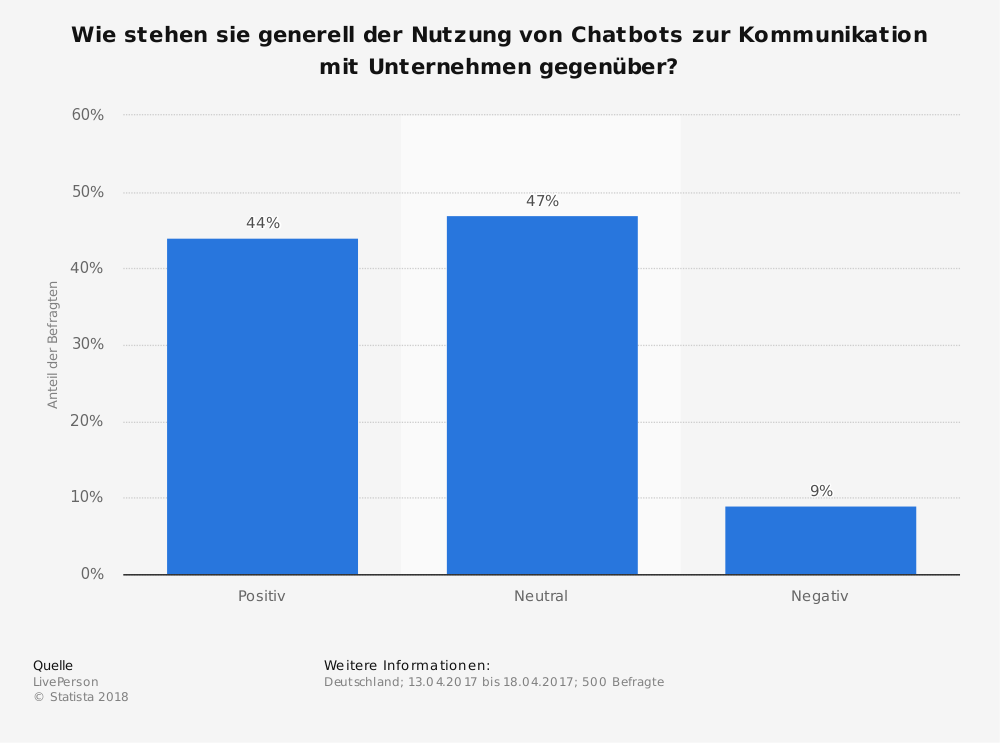
\includegraphics[width=0.6\textwidth]{Anhang/2018_stat_bewertung_chatbots}
  \quelle[o. \pno]{Statista_2019_Bewertung_Chatbots}
  \caption{Bewertung von Chatbots}
\label{fig:bewertungchatbots}
\end{figure}

Auch in Privathaushalten halten Chatbots in Form von Sprachassistenten wie \textit{Amazon Alexa} oder \textit{Google Home} Einzug und an jedem aktuellen Windows-Computer kann mittlerweile \textit{Microsoft Cortana} genutzt werden. Im Rahmen der Heimautomatisierung können so Heizung oder Licht per Sprachinteraktion mit Sprachassistenten bzw. Chatbots gesteuert werden. \footcite[Vgl.][o. \pno]{Kuhn_2015_Sprachassistenten}

% \todo{Puppet Bot, Sprachassistenten im weiteren Sinne Bots}
Da ist es naheliegend, dass man diese Technologie auch im Bereich der Softwareentwicklung oder des Rechenzentrumsbetriebs zur Automatisierung verwenden möchte. GitHub hat dies 2013 erkannt und mit der Vorstellung des Chatbots \textit{Hubot} den Begriff ChatOps, also die Integration eines Chatbots in eine Toolchain oder einen Prozess, geprägt. \footcite[Vgl.][o. \pno]{GitHub_2013_Chatops}

Auch das bekannte, an Unternehmenskunden gerichtete Chat-Tool \acf{Slack} bietet die Möglichkeit, Chatbots zu entwickeln und somit an die eigene Arbeitsumgebung anzupassen. \footcite[Vgl.][o. \pno]{Koeltzsch_2019_Slack}


\section{Umfeld}
Der Autor ist beim \acf{IVZ} beschäftigt, einer Kooperation aller Rundfunkanstalten der \acf{ARD}, sowie Deutschlandradio und \acf{DW} mit Hauptsitz im \acf{rbb}.
Es wurde 1993 als öffentlich-rechtliche Verwaltungsgemeinschaft gegründet und beschäftigt etwa 200 Mitarbeiter an mehreren Standorten.\footcite[Vgl.][o. \pno]{ARD_2018_IVZ}\\
Das \acs{IVZ} bietet seinen Kunden zentral, \acs{ARD}-weite Rechenzentrumsdienstleistungen, wie z. B. SAP oder Archive (Video, Audio, Text) an. Unternehmensweit wird ein Chat-Tool zur Teamkommunikation eingesetzt.


\section{Ziel der Arbeit}
Ziel der vorliegenden Arbeit ist es, zu evaluieren, ob die Einführung einer ChatOps Schnittstelle zur \acf{CMDB} die Arbeit der Mitarbeiter im Rechenzentrumsbetrieb beim Umgang mit dieser erleichtert und angenehmer macht. Bestimmte Aktionen der \acs{CMDB} können in diesem Szenario aus einem Chat-Tool heraus aufgerufen werden und bieten eine Alternative zum Standardweg per Website oder Client. Durch die Befragung von Experten in diesem Gebiet soll beantwortet werden, ob der Einsatz von ChatOps in diesem Zusammenhang nutzenbringend ist.

%"Lässt sich die Arbeit der RZ Mitarbeiter beim Umgang mit der CMDB durch ChatOps erleichtern?"

\section{Abgrenzung}
Nicht Bestandteil dieser Arbeit ist die Evaluierung von ChatOps im Allgemeinen, sowie der Nutzen von ChatOps im gesamten Tätigkeitsspektrum des Rechenzentrumsbetriebs. Der Fokus liegt lediglich auf der Verwendung der CMDB. Außerdem soll nicht der gesamte Funktionsumfang einer \acs{CMDB} betrachtet werden, sondern nur die Komponenten und Funktionen, die im Tagesgeschäft des Rechenzentrumsbetriebs häufig verwendet werden.

\section{Vorgehensweise}
%In \autoref{empg} werden die relevanten empirischen Methoden zur Erforschung des Themas vorgestellt, die Voraussetzung zum Verständnis von \autoref{AnfA} sind.
In \autoref{theg} werden die für das Verständnis der Thematik notwendigen Fachbegriffe eingeführt, erläutert und in einen Zusammenhang gesetzt. In \autoref{AnfA} wird eine Anforderungsanalyse durchgeführt, um die im Arbeitsalltag am meisten genutzten \acs{CMDB} Funktionen zu ermitteln und herauszufinden, in welchen Fällen eine ChatOps Umsetzung möglich und sinnvoll ist. Die Anforderungen werden mithilfe von Experteninterviews ermittelt, wobei die Analyse der Transkripte nach der Methode von Meuser und Nagel erfolgt.\\
In \autoref{Praxis} wird ein Chatbot entworfen und die Interaktion mit der bestehenden \acs{CMDB} beschrieben.
Abschließend wird in \autoref{Fazit} ein Fazit gezogen, es wird aufgrund der in dieser Arbeit gewonnenen Erkenntnisse geschlussfolgert, welchen Nutzen und Vorteil ChatOps im betrachteten Kontext bietet. Darüber hinaus wird ein Ausblick gegeben, wie ChatOps sich in Zukunft entwickeln könnte und in welchen Gebieten (im Rechenzentrum und darüber hinaus) es ebenfalls Fuß fassen könnte.

% \section{Über diese Arbeit}
Diese Arbeit ist in \LaTeX~gesetzt. Die Versionierung wurde mit Git vorgenommen.

% \chapter*{Empirische Grundlagen} \label{empg}
% \section{Anforderungsmanagement}
% \footcite[Vgl.][o. S.]{Grande_2014_Anforderungsmanagement}


% Ziel des Anforderungsmanagements bzw. Requirements Engineerings nach Pohl und Rupp ist die Erfassung und Dokumentation von Anforderungen.\footcite[Vgl.][S. 3]{Pohl_2015_Requirements}
%
% Die Haupttätigkeiten sind die Ermittlung, Dokumentation, Prüfung und Verwaltung von Anforderungen, wobei die Verwaltung mit den drei vorigen Tätigkeiten einher geht. \footcite[Vgl.][S. 4 f.]{Pohl_2015_Requirements}
% %
% \subsection{Ermittlung}
% Bei der Ermittlung der Anforderungen werden verschiedene Quellen, wie z. B. Stakeholder, Dokumente oder aktive Systeme genutzt um Anforderungen zu detektieren und zu verfeinern.\footcite[Vgl.][S. 21]{Pohl_2015_Requirements}\\
% Das Interview ist eine mögliche Befragungstechnik, bei der ein Stakeholder (Interviewpartner) vom Requirements Engineer (Interviewer) vorgegebene Fragen gestellt bekommt. Die Antworten werden protokolliert. Etwaige Rückfragen können sofort im Gesprächsverlauf geklärt werden. Durch geschickt gestellte Fragen können auch unterbewusste Anforderungen ermittelt werden. Der Verlauf des Gesprächs kann individuell angepasst werden, es wird gezielt nachgefragt und auf einzelne Themen eingegangen, um das behandelte Thema möglichst komplett abzubilden.\footcite[Vgl.][S. 28]{Pohl_2015_Requirements}
%
% \subsection{Dokumentation}
% Die erarbeiteten Anforderungen werden in natürlicher Sprache oder in dafür vorgesehenen Modellen dokumentiert, wobei entsprechende Techniken zum Einsatz kommen. \footcite[Vgl.][S. 4]{Pohl_2015_Requirements}\\
% Die im Requirements Engineering anfallenden Tätigkeiten müssen geeignet dokumentiert werden. Dazu zählt z. B. auch die Erstellung von Interviewprotokollen. Als Dokumentation gilt jede Form der formalen Darstellung, von Beschreibung in natürlicher über strukturierten Text bis hin zu formalen Techniken wie Diagrammen. Die Dokumentationsform sollte der zugrundeliegenden Aktivität angemessen sein und diese sinnvoll wiedergeben. \footcite[Vgl.][S. 35 ff.]{Pohl_2015_Requirements}

% \subsection{Prüfung}
% % Um die Qualität der Anforderungen gewährleisten zu können, muss diese frühzeitig geprüft werden.\footcite[Vgl.][S. 4]{Pohl_2015_Requirements}
% Zu den Qualitätskriterien zählen u.A. Korrektheit und Abgestimmtheit. Die Methoden der Qualitätskontrolle können dabei sowohl für einzelne Anforderungen, als auch für Anforderungsdokumente eingesetzt werden.
% Bei der Überprüfung der Anforderungen sollen Fehler wie \glqq{}Mehrdeutigkeit, Unvollständigkeit und Widersprüche\grqq\footcite[][S. 95]{Pohl_2015_Requirements} aufgedeckt werden.\footcite[Vgl.][S. 95]{Pohl_2015_Requirements}

\subsection{Verwaltung}
Die Verwaltung der Anforderungen erfolgt parallel zu den vorher genannten Tätigkeiten und beinhaltet die Strukturierung und Aufbereitung für verschiedene Rollen.\footcite[Vgl.][S. 5]{Pohl_2015_Requirements}\\
Außerdem werden Verfolgbarkeit, Versionierung, Priorisierung und die Verwaltung von Änderungen unter Beibehaltung der Konsistenz sichergestellt. Auch hier reicht der Fokus von Einzelanforderungen bis hin zu Anforderungskatalogen.
Die Anforderungen werden mit den Informationen Identifikator, Name, Autor und Quelle versehen. Die Priorisierung der Anforderungen kann z. B. durch den Auftraggeber oder Faktoren wie die Dringlichkeit der Umsetzung geschehen.\footcite[Vgl.][S. 126]{Pohl_2015_Requirements}

% \section{Qualitative Inhaltsanalyse}
% \footcite[Vgl.][S.]{Mayring_2009_qualitative_Inhaltsanalyse}

% \todo{Systematisierendes Interviews --> Qualitative Inhaltsanalyse}
% \question{Muss ich die qualitative Inhaltsanalyse erläutern oder reicht das Experteninterview?}

Die qualitative Inhaltsanalyse nach Mayring ist eine Technik zur Auswertung und Interpretation von Text. Sie kann als eigenständige Erhebungsmethode betrachtet werden und hat zum Ziel, Kategorien aus Textbestandteilen zu bilden und den Inhalt sinngemäß zusammenzufassen. \footcite[Vgl.][S. 671]{Mayring_2009_qualitative_Inhaltsanalyse}\\
Das Experteninterview ist eine Möglichkeit, die qualitative Inhaltsanalyse durchzuführen und beinhaltet u.a. Audioaufnahme und Transkription.\footcite[Vgl.][S. 673 f.]{Mayring_2009_qualitative_Inhaltsanalyse}

In dieser Arbeit wird das Experteninterview als spezielle Form der qualitativen Inhaltsanalyse verwendet. Auf eine Detailbeschreibung dieser wird daher verzichtet und das Experteninterview dafür in \autoref{Experteninterview} ausführlich beschrieben.

% \section{Experteninterview} \label{Experteninterview}
Heutzutage ist die Bedeutung von Experteninterviews in der Forschungspraxis unumstritten. In verschiedensten Bereichen gehört es fest zum Kernbestand der alltäglichen Forschungsroutine, sei es als eigenständige Erhebungsmethode oder als ergänzende Methode im Rahmen explorativer Forschung. \footcite[Vgl.][S. 1]{Bogner_2014_Interview}

% Wesentliche Funktionen des Experteninterviews sind Informationsgewinnung und Theorieentwicklung, weswegen es sich als Methode eignet, um Anforderungen zu erheben.
% \footcite[Vgl.][S. 187 f.]{Glaeser_2010_Inhaltsanalyse}$^,$\footcite[Vgl.][S. 9]{Bogner_2014_Interview}
%
% Wenn von Experteninterviews die Rede ist, kann man davon ausgehen, dass ein leitfadengestütztes, qualitatives Interview gemeint ist. Da das Instrument Experteninterview dem Forschungsvorhaben angepasst werden muss, können jedoch verschiedene Dinge unter dem Begriff verstanden werden und es ist nötig klarzustellen, welche Ausprägung gemeint ist.\footcite[Vgl.][S. 3]{Bogner_2014_Interview}
% Auch der Expertenbegriff muss der Forschungsfrage angepasst werden.\footcite[Vgl.][S. 180]{Meuser_1994_Interview}

% In dieser Arbeit wird ausschließlich der qualitativ ausgerichtete Ansatz von Meuser und Nagel verfolgt. Quantitative Ansätze oder qualitative Ansätze anderer Autoren, die von dem behandelten abweichen werden hier nicht weiter ausgeführt.\footcite[Vgl.][o.S.]{Meuser_2010_Interview}

% Um das Experteninterview anwenden zu können, muss geklärt werden, wer als Experte gilt, was Expertenwissen bedeutet und wie man es abruft, welche Schritte zur Vorbereitung eines Interviews erforderlich sind, welche Gesprächsführung für die Forschungsfrage Sinn macht und wie die Interviews ausgewertet werden können.\footcite[Vgl.][S. 6 f.]{Bogner_2014_Interview}


% \subsection{Arten}
% Meuser und Nagel unterscheiden Experteninterviews grundlegend in systematisierende und explorativ-felderschließende Interviews. Bei ersteren wird der Experte zu seinem eigenen Fachgebiet befragt (Betriebswissen), bei letzerem liefert er lediglich \glqq{}Informationen über die Kontextbedingungen des Handelns der Zielgruppe\grqq (Kontextwissen)\footcite[][S.445]{Meuser_1991_Interview} .
%
% Bogner, Littig und Menz sprechen in diesem Zusammenhang von fundierenden und explorativen Interviews und fasst die vormals genannten Kategorien unter dem Begriff \textit{informatorisch} zusammen. Außerdem ergänzt er zwei  deutungswissenorientierten Varianten. Eine genaue Aufschlüsselung ist in \autoref{tab:artenei} zu sehen.\footcite[Vgl.][S. 445 f.]{Meuser_1991_Interview}$^,$\footcite[Vgl.][S. 22 ff.]{Bogner_2014_Interview}
%
%
% \begin{table}[H]
% \centering
% \begin{tabularx}{1\textwidth}{XXX}%
%                             & Explorativ (Kontextwissen) & Fundierend (Betriebswissen) \\\midrule
%    Informatorisch           & Explorative Datensammlung & Systematisierendes Interview \\
%    Deutungswissenorientiert & Exploration von Deutungen & Theoriegenerierendes Interview
% \end{tabularx}
%   \\\quelle{Bogner_2014_Interview}
%   \\\quelle{Meuser_1991_Interview}
% \caption{Arten von Experteninterviews}
% \label{tab:artenei}
% \end{table}


\subsection{Phasen}
% Ein Experteninterview kann aus bis zu acht Phasen bestehen, diese sind in \autoref{tab:phasenei} aufgeführt und anschließend im Detail erläutert. Für die Abfrage von Betriebswissen müssen alles Phasen durchlaufen werden, bei Kontextwissen entfallen die letzten beiden.\footcite[Vgl.][S. 466 f.]{Meuser_1991_Interview}

\begin{table}[ht]
\centering
\begin{tabularx}{1\textwidth}{llX}%
Nr. & Phase                            & Aktivitäten \\\midrule
1   & Leitfadenerstellung              & Erstellung des Leitfadens\\
2   & Tonaufnahme                      & Aufzeichnung des Gesprächs\\
3   & Transkription                    & Übertragung in Schriftdeutsch\\
4   & Paraphrase                       & Zusammenfassung und thematische Einteilung\\
5   & Überschriften                    & Verdichtung, Betitelung der paraphrasierten Abschnitte\\
6   & Thematischer Vergleich           & Vergleich aller Intervews, Suche nach Gemeinsamkeiten\\
7   & Soziologische Konzeptualisierung & Systematisierung, Typisierung, Deutung \\
8   & Theoretische Generalisierung     & Bildung von Theorien, Interpretation der Ergebnisse
\end{tabularx}
  \\\quelle{Meuser_1991_Interview}
\caption{Phasen eines Experteninterviews}
\label{tab:phasenei}
\end{table}

% \subsubsection{Transkription}
% Das Hauptaugenmerk von Experteninterviews liegt auf der Gewinnung von Wissen. Daher ist eine mühselige Notation, wie sie bei narrativen Interviews vorgenommen wird nicht nötig. Elemente wie Pausen, Betonung oder Stimmlage werden nicht interpretiert.
% Eine Transkription wird in der Regel nicht für die gesamte Tonaufnahme durchgeführt, sondern kann selektiv erfolgen. Bei der Abfrage von Betriebswissen fällt die Transkription umfangreicher aus als bei Kontextwissen. \footcite[Vgl.][S. 455 f.]{Meuser_1991_Interview}
%
% \subsubsection{Paraphrase}
% Die Paraphrase erfolgt unter Berücksichtigung der Forschungsfrage und gibt die Aussagen der Experten chronologisch geordnet und unverfälscht wieder, wobei diese zu thematischen Verbünden zusmamengefasst werden. Ob die Passage zusammenfassend oder detailliert wiedergegeben wird hängt von der Priorität des Themas und nicht zwangsläufig von der ihm gewidmeten Zeit ab.\footcite[Vgl.][S. 456 f.]{Meuser_1991_Interview}
%
% \subsubsection{Überschriften}
% Die paraphrasierten Abschnitte werden möglichst textnah mit einer oder mehreren Überschriften versehen, je nach dem, wie viele Themen angesprochen werden. Dabei ist darauf zu achten, dass das Expertenwissen im Fokus steht, der Experte als Person ist nicht relevant.\footcite[Vgl.][S. 458 f.]{Meuser_1991_Interview}

% \subsubsection{Thematischer Vergleich}
% Ab diesem Schritt werden nicht mehr die Interviews im Einzelnen betrachtet, es erfolgt ein Vergleich der thematisch ähnlichen Textpassagen aller Interviews, wobei die Überschriften nach Möglichkeit vereinheitlicht werden. Es wird geprüft, ob sich die Äußerungen der Experten decken oder ob sie unterschiedliche Ansichten haben. Außerdem wird betrachtet, zu welchen Themen sich alle Experten äußern und zu welchen nur einzelne.\footcite[Vgl.][S. 459 f.]{Meuser_1991_Interview}$^,$\footcite[Vgl.][S. 37]{Matthes_1986}
%
\subsubsection{Soziologische Konzeptualisierung}
In diesem Schritt werden aus dem gemeinsamen Wissen der Experten Kategorien gebildet, wodurch eine weitere Verdichtung des Wissens erfolgt. Dadurch soll eine Typisierung, Verallgemeinerung und Deutung des Wissens möglich werden. Die Struktur des Expertenwissens wird betrachtet, wodurch die Reichweite der Konzepte geprüft werden kann.\footcite[Vgl.][S. 462 f.]{Meuser_1991_Interview}

\subsubsection{Theoretische Generalisierung}
Im letzten Schritt werden Theorien aus Sinnzusammenhängen gebildet und die Ergebnisse interpretiert, wobei darauf zu achten ist, dass man sich nicht von Verdachten leiten lässt, sonder nur mit dem Forschungsmaterial arbeitet.\footcite[Vgl.][S. 463 ff.]{Meuser_1991_Interview}




\subsection{Definition: Experte}
% Das Wort \textit{Experte} leitet sich aus dem lateinischen \textit{expertus} (erprobt, bewährt) ab, welches wiederum aus dem passiven Verb \textit{experiri} (prüfen, ausprobieren) gebildet wird. Experten sind also Fachleute und Kenner, bzw. allgemein gesprochen Personen, die über ein gewisses Spezialwissen verfügen, das auf der Erfahrung des ausgiebigen Prüfens und Ausprobierens fußt. \footcite[Vgl.][S. 9]{Bogner_2014_Interview}
%
% Wie in \autoref{fig:experte} zu erkennen, zeichnet sich ein Experte durch eine bestimmte Kombination von Macht und Wissen aus, welche ihn von Eliten, Spezialisten und spezialisierten Laien unterscheidet.\\ \glqq{}Der Experte ist -- im Gegensatz zum Spezialisten – nicht allein durch Sonderwissen in Form fachspezifischer Kompetenzen charakterisiert, sondern durch seine Fähigkeit, Verbindungen zu anderen Wissensbeständen und Wissensformen herzustellen und die Relevanz des eigenen Wissens zu reflektieren\grqq. \footcite[][S. 14]{Bogner_2014_Interview}$^,$\footcite[Vgl.][S. 21 f.]{Hitzler_1994}
%
% \begin{figure}[H]
%   \centering
%   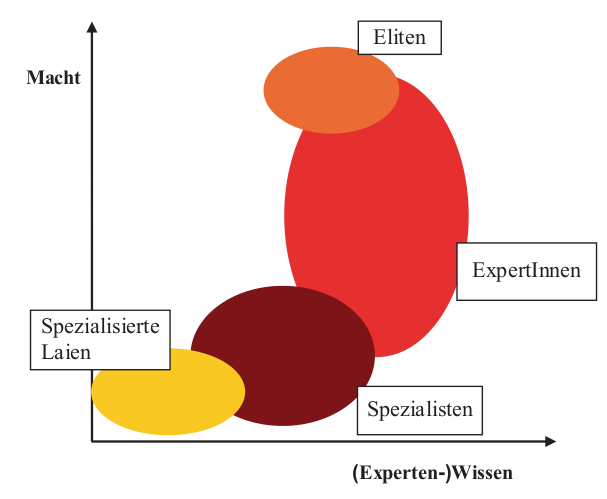
\includegraphics[width=0.6\textwidth]{Anhang/Experte}
%   \\\quelle{Littig_2008}
%   \caption{Experteneinordnung}
% \label{fig:experte}
% \end{figure}
%
% Gläser und Laudel definieren Experten als Menschen, die ein besonderes Wissen über soziale Sachverhalte besitzen.\footcite[Vgl.][S. 12]{Glaeser_2010_Inhaltsanalyse} Man könnte nun davon ausgehen, dass jeder ein Experte ist, da er sich in seinem Fachgebiet gut auskennt. Genauer betrachtet  gibt es jedoch große Unterschiede zwischen Laien und Experten, man bedenke nur das Verhältnis zwischen Ärzten und Patienten. Ein solcher Expertenbegriff ist also zu weit gefasst und es kann nicht jedes qualitative Interview automatisch als Experteninterview bezeichnet werden.\footcite[Vgl.][S. 10 f.]{Bogner_2014_Interview}
%
% Meuser und Nagel hingegen betrachten den Experten als Konstrukt des Forschungsinteresses. Die Expertise ist also keine allgemeingültige Eigenschaft oder Fähigkeit einer Person, sondern eine Zuschreibung des Forschenden an diese, im speziellen Kontext der Forschungsfrage. \footcite[Vgl.][S. 181]{Meuser_1994_Interview}
%


\subsection{Definition: Expertenwissen}
Als einer der ersten hat Schütz das Expertenwissen als sicheres und eindeutiges Wissen beschrieben, das dem Experten \glqq{}jederzeit kommunikativ und reflexiv\grqq\footcite[][S. 12]{Bogner_2014_Interview} verfügbar ist.\footcite[Vgl.][S. 86 ff. ]{Schuetz_1972}
Sprondel ergänzte anschließend, dass das Expertenwissen komplex integrierte Wissensbestände umfasst und auf den professionellen Funktionskontext bezogen ist.\footcite[Vgl.][S. ]{Sprondel_1979}

Expertenwissen spielt in der modernen Gesellschaft eine wichtige Rolle in allen Lebensbereichen, nicht nur in der Wissenschaft. Z. B. Fragen der Gesundheit oder Ernährung werden nicht intuitiv entschieden, sondern auf Basis von Expertise. Dieser Umstand stellt zwar eine Abhängigkeit dar, trägt jedoch dazu bei, dass unsere heutige Gesellschaft eine Wissensgesellschaft mit starker Spezialisierung ist.\footcite[Vgl.][o.S.]{Coser_1992}$^,$\footcite[Vgl.][S. 10]{Bogner_2014_Interview}
% \todo{Seite suchen: Giddens1991}
Umgekehrt betrachtet stellte Nowotny fest, dass die Expertise heutzutage nicht nur in der Wissenschaft, sondern in allen Bereichen der Gesellschaft gebildet wird.\footcite[Vgl.][S. 215 ff. ]{Nowotny_2001}$^,$\footcite[Vgl.][S. 10]{Bogner_2014_Interview}
%
% Das Interessante am Expertenwissen ist nicht nur das Wissen an sich, sondern die Wirkung in der Praxis. Experten werden gefragt, weil ihre Entscheidungen und Ratschläge das Handeln anderer Akteure mitstrukturieren und -gestalten.\footcite[Vgl.][S. 13]{Bogner_2014_Interview} Bogner spricht davon, dass Expertenwissen \glqq seine Bedutung über [...] soziale Wirkmächtigkeit\grqq{} erhält.\footcite[][S. 13]{Bogner_2014_Interview}
% Ferner folgert er daraus die Definition:\\ \glqq Experten lassen sich als Personen verstehen, die sich -- ausgehend von einem spezifischen Praxis- oder Erfahrungswissen, das sich auf einen klar begrenzbaren Problemkreis bezieht -- die Möglichkeit geschaffen haben, mit ihren Deutungen das konkrete Handlungsfeld sinnhaft und handlungsleitend für Andere zu strukturieren.\grqq{}\footcite[][S. 13]{Bogner_2014_Interview}
%

% \subsection{Vorbereitung des Interviews}
%   \todo{Erstellung des Leitfadens}
% \subsection{Wahl der Gesprächsführung}
% \subsection{Auswertung der Interviews}
%
% \footcite[Vgl.][S. 448 f.]{Meuser_1991_Interview}
%   \todo{Auswertung, Transkription, Paraphrase, Überschriften, Theoretischer Vergleich,}
%

% \footcite[Vgl.][o. S.]{Burger_2011_Interview}



\chapter{Grundlagen} \label{theg}
\section{Chatbots}
Ein Chatbot ist ein Programm, das für den Dialog mit Menschen erdacht ist und natürliche Sprache als Text oder Audio entgegennehmen und verarbeiten kann.
Chatbots werden hauptsächlich auf Websites und Instant-Messaging Systemen eingesetzt.
Benutzereingaben werden angenommen und passende Antworten dazu ausgegeben. Außerdem sollen Chatbots Gäste begrüßen und die Unterhaltung in Gang halten.\\
Chatbots können rein regelbasiert oder \acf{KI}-gesteuert reagieren.\\
Durch die inhärente Automatisierung sind Chatbots relevant bezüglich der \glqq{}Unterstützung und Ersetzung von Arbeitskräften\grqq
\footcite[][o. \pno]{Bendel_2018_Chatbot_Definition}{}.
\footcite[Vgl.][o. \pno]{Bendel_2018_Chatbot_Definition}

Chatbots können mit realen Personen oder anderen Chatbots kommunizieren. Ein Chatbot ist jeweils für einen bestimmten Aufgabenbereich vorgesehen und deckt nicht das gesamte Spektrum der menschlichen Kommunikation ab. Ähnlich wie bei Avataren können Chatbots eine \glqq{}körperliche Erscheinung\grqq
\footcite[][71\psq]{de_Vries_2006}
und \glqq{}virtuelle Identität\grqq
\footcite[][71\psq]{de_Vries_2006}
bzw. Charakter haben.
\footcite[Vgl.][71\psq]{de_Vries_2006}

Im Gegensatz zu Agenten arbeiten Chatbots nicht autonom, sondern reaktiv. Sie sind also auf die Befehle von Menschen angewiesen.
\footcite[Vgl.][69\psqq]{de_Vries_2006}

Entscheidend für die Gesprächskompetenz von Chatbots ist das zugrundel iegende Wissen. Die eingesetzten Algorithmen spielen nur eine nachgelagerte Rolle.\\
Für komplexere Problemstellungen  kann es nötig werden, den Kontext genauer zu erfassen. Dazu kann die Gesprächshistorie berücksichtigt und Laufzeitvariablen pro Nutzer gespeichert werden.
\footcite[Vgl.][82\psq]{Feindt_2006_Agenten}

\subsection{Komponenten}
Die wesentlichen Komponenten eines Chatbots sind Utterances (Äußerungen), Intents (Absichten) und Entities (Entitäten).\\
Als Äußerungen gelten alle Eingaben des Nutzers in ihrer Basisausprägung, z. B. \textit{Wie wird das Wetter?}.
Aus der Äußerung wird eine Absicht interpretiert, in diesem Beispiel eine Funktion, die das aktuelle Wetter anzeigt.
Entitäten sind Zusatzparameter für Äußerungen und werden der, mit der Absicht verknüpften Funktion übergeben. Z. B. \textit{Wie wird das Wetter morgen?}, wobei \textit{morgen} die Entität ist.
\footcite[Vgl.][51]{Groetz_2018_Sprich_mit_mir}

\subsection{Arten}
Chatbots werden grundsätzlich als regelbasiert oder selbstlernend kategorisiert.
\footcite[Vgl.][51\psq]{Groetz_2018_Sprich_mit_mir}
\subsubsection{Regelbasiert}
Regelbasierte Chatbots verfügen über einen festen Regelbaum und können nur vordefinierte Fragen beantworten und auf bestimmte Schlüsselwörter reagieren.\\
Wenn der Nutzer sich vertippt, die Fragen leicht anders formuliert oder nicht die richtigen Schlüsselwörter verwendet, kann der Bot daraus keine Aktion ableiten.
\footcite[Vgl.][51\psq]{Groetz_2018_Sprich_mit_mir}
\subsubsection{Selbstlernend}
Durch den Einsatz von \acs{KI} und maschinellem Lernen können Chatbots menschliche Sprache besser verstehen und es muss nicht jede Formulierung eines Satzes angelernt werden. Die Komplexität ist bei dieser Variante höher.
Allerdings können dann Richtigkeit und Qualität der Antworten nicht mehr sichergestellt werden, bzw. die Absicht des Benutzers wird möglicherweise falsch interpretiert.
\footcites[Vgl.][151\psq]{Feindt_2006_Gespraechskompetenz}[Vgl.][51\psq]{Groetz_2018_Sprich_mit_mir}

\subsection{Sonderfall Sprachassistenten}
Als Sonderform der Chatbots können Sprachassistenten betrachtet werden, die sich spätestens seit der Einführung von Amazon Alexa, Google Assistant und Apple Siri großer Beliebtheit erfreuen.
\\
Die Steuerbefehle werden dabei nicht textuell, sondern verbal übergeben und müssen in der Regel durch ein Schlüsselwort wie \textit{Okay Google} oder \textit{Alexa} eingeleitet werden.\\
Dank der Auslagerung der Spracherkennung in die Cloud hat sich die Qualität dieser erheblich verbessert. Das Anlernen von Klangfarbe und Fachvokabular muss nicht mehr individuell manuell vorgenommen werden, sondern geschieht aggregiert in der Cloud.\\
Als zusätzliche Herausforderungen im Vergleich zur textuellen Variante existieren bei Sprachassistenten \glqq{}Dialekte, Sprachfehler und Umgebungsgeräusche\grqq
\footcite[][64]{Puscher_2018_Gut_zugehoert}{}.
\footcites[Vgl.][64]{Puscher_2018_Gut_zugehoert}[Vgl.][50]{Groetz_2018_Sprich_mit_mir}

\subsection{Charakter}
Wichtig für die Akzeptanz eines Chatbots ist, ihm einen Charakter zu verleihen. Es sollte früh entschieden werden, ob er sachlich, empathisch oder frech sein soll.\\
Zu den Eigenschaften zählen Alter, Geschlecht, Erscheinung (Mensch, Tier, Maschine), Zweck und Geschichte bzw. Herkunft.\\
Merkmale wie Humor, Offenheit, Redseligkeit, Auftreten (laut, leise, frech) und Ähnlichkeit mit bekannten Figuren (z. B. Comicfiguren) sollten auch geplant werden.\\
Eine Möglichkeit ist, das Firmenmaskottchen als Chatbot umzusetzen, allerdings sollte abgewägt werden, ob es die nötige Kompetenz verkörpert.
\footcite[Vgl.][68\psq]{Puscher_2018_Gut_zugehoert}




\section{ChatOps}
Der Begriff ChatOps stammt aus dem DevOps-Umfeld und wurde von GitHub durch die Einführung ihres Chatbots \textit{Hubot} im Jahr 2013 geprägt. Jesse Newland, der damals den Vortrag hielt spricht von \glqq{}placing tools
directly in the middle of the conversation\grqq
\footcite[Vgl.][62]{GitHub_2013_Chatops},
also davon, die im Unternehmen genutzten Tools direkt im Chatroom verfügbar zu machen.
\footcite[Vgl.][o. \pno]{Sigler_2014_Chatops}

\subsection{Grundgedanke}
Unter ChatOps wird die Verbindung von Chatbots mit operativen Prozessen verstanden. Dies geschieht durch die transparente Verbindung von Mitarbeitern, Tools, Prozessen und Automatisierung.
Dabei entsteht eine kollaborative Arbeitsumgebung, bei der für alle Mitarbeiter ersichtlich ist, woran gerade wie gearbeitet wird und ermöglicht eine ausführliche Historie der Tätigkeiten und der beteiligten Personen.
\footcites[Vgl.][o. \pno]{Zyane_2017_ChatOps}[Vgl.][190]{Betz_2016_Digital}

Als Grundsatz von ChatOps gilt die \acf{CAMS}, also eine Kultur, die Automatisierung, Messbarkeit und Transparenz mit sich bringt. Dieser Gedanke wurde dem DevOps Umfeld entliehen.
\footcite[Vgl.][o. \pno]{Zyane_2017_ChatOps}

Wenn Fehler auftreten, kann direkt geprüft werden, ob und welche Änderungen am System vorgenommen wurden und nicht alle Mitarbeiter müssen einzeln befragt werden.\\
Auch bei der Einarbeitung von neuen Mitarbeitern ist die Transparenz hilfreich, da sie sämtliche Arbeitsabläufe ihres Teams mitverfolgen können und dazu nicht einmal am gleichen Standort sein müssen. Sie können einfach den Räumen beitreten, die für ihre Rollen und Verantwortlichkeiten vorgesehen sind.
\footcites[Vgl.][o. \pno]{Sigler_2014_Chatops}[Vgl.][66]{Hand_2016_ChatOps}

Durch anpassbare Skripte und Plugins können individuelle Prozesse aus dem Chatroom heraus angestoßen werden. So kann z. B.~in einem Softwareprojekt das Code Deployment gestartet werden oder in der IT-Security auf gemeldete Sicherheitsvorfälle reagiert werden. Außerdem können Benachrichtigungen an die Teammitglieder versendet werden, die gerade zuständig sind.
\footcite[Vgl.][o. \pno]{Sigler_2014_Chatops}

\subsection{Komponenten}
Um ChatOps einführen zu können, müssen als Kernkomponenten ein Kollaborationswerkzeug, ein Bot und eine Systemintegration gegeben sein.\\
Ein Kollaborationswerkzeug ist das Chat-Tool, in dem Stakeholder miteinander kommunizieren können und in Teams organisiert sind.\\
Ein Bot im ChatOps-Kontext bildet die Brücke zwischen Kollaborationswerkzeug und Systemwerkzeugen. Er erhält von den Teammitgliedern natürlichsprachige Befehle in Textform, interpretiert diese und fragt dann die angeforderte Information vom verbundenen System ab bzw. führt die angeforderte Aktion aus.\\
Als Systemintegration kommt jedes Tool in Frage, das von einem Unternehmen genutzt wird und eine Schnittstelle nach außen bietet, die vom Bot genutzt werden kann.
\footcite[Vgl.][o. \pno]{Zyane_2017_ChatOps}


Die beschriebenen Zusammenhänge sind in \autoref{fig:cop} ersichtlich. Das Team arbeitet mit einem Kollaborationswerkzeug und die Automatisierung und Anbindung an die Systeme wird von einem Bot sichergestellt.

\begin{figure}[H]
  \centering
  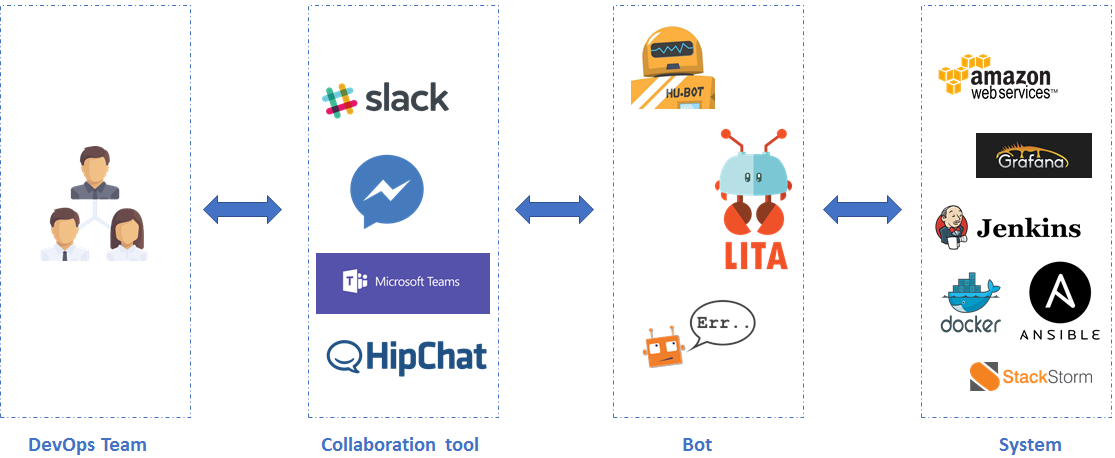
\includegraphics[width=\textwidth]{Anhang/cop}
  \quelle[o. \pno]{Zyane_2017_ChatOps}
  \caption{ChatOps Prozess}
\label{fig:cop}
\end{figure}


\subsubsection{Kollaborationswerkzeug}
Bekannte Beispiele für Kollaborationswerkzeuge sind Slack, Atlassian HipChat oder Cisco WebEx Teams, die allesamt die Integration von Bots ermöglichen.
Ziel solcher Werkzeuge ist es, Kollaboration zu ermöglichen, die Kommunikation von Arbeitsteams effektiv zu gestalten und klassische Kanäle wie E-Mail oder SMS abzulösen. Dabei ist auch die Anbindung von anderen Diensten, wie z. B. Cloud Speicher zur kollaborativen Bearbeitung von Dokumenten möglich. So müssen Unternehmen nicht zwangsläufig die Software von einem bestimmten Hersteller beziehen, sondern können das Kollaborationswerkzeug ihrer Wahl an verschiedene Dienste anbinden.
\footcites[Vgl.][o. \pno]{Zyane_2017_ChatOps}[Vgl.][o. \pno]{Koeltzsch_2019_Slack}

Slack zum Beispiel gilt als erfolgreichstes Kollaborationswerkzeug. Das Unternehmen wurde 2013 gegründet und hat heute 8 Millionen Nutzer, davon 3 Millionen zahlende und der Marktwert wird auf 7,1 Milliarden Dollar geschätzt. In der Basisversion ist es kostenlos, für Features wie längeres Vorhalten der Chatverläufe muss eine Lizenz erworben werden.
Zum Februar 2019 hat Slack den Konkurrenten HipChat abgeschaltet und die bisherigen Kunden nach Slack migriert, nachdem dieser Ende 2018 übernommen wurde.
\footcites[Vgl.][o. \pno]{Koeltzsch_2019_Slack}[Vgl.][o. \pno]{Donath_2018_Hipchat_Uebernahme}

\subsubsection{Bot}
Als ChatOps Bots können z. B. Hubot, Lita, oder  Errbot verwendet werden, wobei alle in etwa die gleiche Funktionalität besitzen, da sie sich am ursprünglichen ChatOps Bot Hubot orientieren.
Allerdings sind sie in verschiedenen Sprachen geschrieben, was für die Weiterentwicklung und Anbindung an Systeme wichtig sein kann, und weisen einige Besonderheiten auf. Eine Übersicht ist in \autoref{tab:bots} zu sehen.
\footcite[Vgl.][o. \pno]{Zyane_2017_ChatOps}

Cog hingegen ist ein Bot Framework, das möglichst plattformunabhängig arbeitet und ähnlich der Unix Funktion \textit{Pipe} funktioniert, also eine Verknüpfung verschiedener Befehle in beliebiger Komplexität ermöglicht.
\footcite[Vgl.][o. \pno]{Zyane_2017_ChatOps}

\begin{table}[H]
\centering
\begin{tabularx}{.8\textwidth}{l|l|X}
  Name & Sprache & Besonderheiten\\\hline
  Hubot & CoffeeScript & große Community\\
  Lita & Ruby & viele Plugins\\
  Errbot & Python & einfache Integration von APIs\\
  Cog & (Framework) & Unix-ähnliches Piping\\
\end{tabularx}
\quelleeigen[o. \pno]{Zyane_2017_ChatOps}
\caption{Verschiedene ChatOps Bots}
\label{tab:bots}
\end{table}

%\begin{table}[H]
%\centering
%\begin{tabularx}{1\textwidth}{|l|l|X|}\hline
%  Name & Sprache & Besonderheiten\\\hline\hline
%  Hubot & CoffeeScript & große Community\\\hline
%  Lita & Ruby & viele Plugins\\\hline
%  Errbot & Python & einfache Integration von APIs\\\hline
%  Cog & (Framework) & Unix-ähnliches Piping\\\hline
%\end{tabularx}
%\quelleeigen[o. \pno]{Zyane_2017_ChatOps}
%\caption{Verschiedene ChatOps Bots}
%\label{tab:bots}
%\end{table}

\subsubsection{Systemintegration}
Ein Chatbot kann z. B. an das Ticketsystem, Versionskontrollsystem, Konfigurationsmanagementsystem oder Monitoringsystem angebunden werden, um dort automatisiert Aufgaben auszuführen. Eine Auflistung mit Beispielen ist in \autoref{tab:integrations} zu finden.
\footcite[Vgl.][o. \pno]{Zyane_2017_ChatOps}

\begin{table}[H]
\centering
\begin{tabularx}{.8\textwidth}{l|X}
  System & Beispiele \\\hline
  Ticket& JIRA, OTRS, TeamForge \\
  Versionskontrolle & GitHub, GitLab, Bitbucket\\
  Konfigurationsmanagement & Ansible, Salt, Chef, Puppet\\
  Monitoring & Nagios, Check\_MK, Grafana, Prometheus, Kibana\\
  Continuous Integration & Jenkins, Travis CI, Bamboo\\
  \acf{IaC} & Docker, Swarm, Kubernetes, Terraform, Vagrant\\
\end{tabularx}
\quelleeigen[o. \pno]{Zyane_2017_ChatOps}
\caption{ChatOps Systemintegrationen}
\label{tab:integrations}
\end{table}

%\begin{table}[H]
%\centering
%\begin{tabularx}{1\textwidth}{|l|X|}\hline
%  System & Beispiele \\\hline\hline
%  Ticket& JIRA, OTRS, TeamForge \\\hline
%  Versionskontrolle & GitHub, GitLab, Bitbucket\\\hline
%  Konfigurationsmanagement & Ansible, Salt, Chef, Puppet\\\hline
%  Monitoring & Nagios, Check\_MK, Grafana, Prometheus, Kibana\\\hline
%  Continuous Integration & Jenkins, Travis CI, Bamboo\\\hline
%  \acf{IaC} & Docker, Swarm, Kubernetes, Terraform, Vagrant, Packer\\\hline
%\end{tabularx}
%\quelleeigen[o. \pno]{Zyane_2017_ChatOps}
%\caption{ChatOps Systemintegrationen}
%\label{tab:integrations}
%\end{table}

\section{CMDB}
Eine \acf{CMDB} ist ein aus dem \acf{ITIL} Umfeld stammendes Modell, um die IT-Infrastruktur eines Unternehmens abzubilden. Mit ihr kann auf Informationen zu Diensten und Konfigurationen zugegriffen werden.
\footcite[Vgl.][70\psq]{Olbrich_2008_ITIL}

Neben Hardware und Infrastruktur werden auch Dokumente wie Verträge, \acfp{SLA} oder Notfallpläne, sowie  Personen und Prozesse dort dokumentiert.
\footcite[Vgl.][253]{Sturm_2017_CMDB}


Die Komponenten einer \acs{CMDB} werden als \acfp{CI} bezeichnet. Ein \acf{CI} ist eine Einheit, die aus einem oder mehreren Objekten bestehen kann. Also z. B.~eine CPU, ein Kabel, ein kompletter Server, ein Netzwerksegment oder ein Cluster.
\footcite[Vgl.][70\psq]{Olbrich_2008_ITIL}

Zu den \acsp{CI} wird geplant, welchen Zweck diese erfüllen und in welchem Kontext sie eingesetzt werden (technisch und organisatorisch).
Es kann identifiziert werden, wer für das \acs{CI} zuständig ist und in welcher Version es vorliegt.
Sämtliche Änderungen an \acsp{CI} werden dokumentiert, wodurch eine vollständige Änderungshistorie über den gesamten Lebenszyklus entsteht.
\footcite[Vgl.][70\psq]{Olbrich_2008_ITIL}

Ein \acs{CI} kann verschiedene Eigenschaften bzw. Attribute besitzen und es können Verlinkungen zu anderen \acsp{CI} hergestellt werden, wodurch die Bildung einer Objekthierarchie möglich ist. Eine beispielhafte Anordnung ist in \autoref{fig:cih} zu sehen. \acsp{CI} werden außerdem in eine Kategorie eingeordnet und es kann ein Status zugewiesen werden.
\footcite[Vgl.][72\psqq]{Olbrich_2008_ITIL}

\begin{figure}[H]
  \centering
  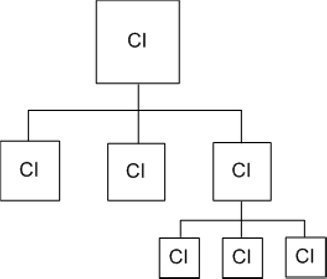
\includegraphics[width=0.3\textwidth]{Anhang/cih}
  \quelle[74]{Olbrich_2008_ITIL}
  \caption{Configuration Item Beziehungen}
\label{fig:cih}
\end{figure}


Neben rein hierarchischer Untergliederung sind auch andere Beziehungen zwischen \acsp{CI} möglich. Eine Übersicht mit Beispielen ist in \autoref{tab:bezci} zu sehen.\\
Durch die Verknüpfungen entsteht eine Übersicht, welche Systeme bei kritischen Ereignissen betroffen sind. Z. B.~welche Auswirkungen der Ausfall eines Switches hat.
\footcite[Vgl.][74\psq]{Olbrich_2008_ITIL}

\begin{table}[H]
\centering
\begin{tabularx}{0.8\textwidth}{l|X}
                            Beziehung & Beispiel \\\hline
                            X ist Teil von Y & eine CPU ist Teil eines Servers\\
                            X ist verbunden mit Y & ein Server ist mit einem Storagesystem verbunden \\
                            X benutzt Y & zwei Netzwerke benutzen eine VPN Verbindung \\
                            X ist eine Ausprägung von Y & gleicher Server, andere RAM Bestückung \\
\end{tabularx}
\quelleeigen[74]{Olbrich_2008_ITIL}
\caption{Beziehungen zwischen \aclp{CI}}
\label{tab:bezci}
\end{table}

%\begin{table}[H]
%\centering
%\begin{tabularx}{1\textwidth}{|l|X|}\hline
%                            Beziehung & Beispiel \\\hline\hline
%                            X ist Teil von Y & eine CPU ist Teil eines Servers\\\hline
%                            X ist verbunden mit Y & ein Server ist mit einem Storagesystem verbunden \\\hline
%                            X benutzt Y & zwei Netzwerke benutzen eine VPN Verbindung \\\hline
%                            X ist eine Ausprägung von Y & gleicher Server, andere RAM Bestückung \\\hline
%\end{tabularx}
%\quelleeigen[74]{Olbrich_2008_ITIL}
%\caption{Beziehungen zwischen \aclp{CI}}
%\label{tab:bezci}
%\end{table}


Jedes \acs{CI} durchläuft einen Lebenszyklus, der aus Beschaffung (Procurement), Betrieb (Operating) und Entsorgung (Disposal) besteht.
Die Beschaffung beinhaltet Bestellung und Lieferung. Sobald das \acs{CI} betriebsbereit ist, geht es in die Betriebsphase und wenn es ausgemustert wird, geht es in die Entsorgungsphase.\\
Je nach Phase können die \acsp{CI} verschiedene Zustände einnehmen. Diese können einen veränderbaren (V) oder finalen (F) Status haben. Eine Übersicht der Zustände pro Phase ist in \autoref{tab:statci} zu sehen.
\footcite[Vgl.][76\psq]{Olbrich_2008_ITIL}

\begin{table}[H]
\centering

\textit{Beschaffung}\\
\begin{tabularx}{.8\textwidth}{p{2cm}|c|X}
    Status      &  Art & Beschreibung                          \\\hline
    ordered     &  V & Bestellung wurde ausgelöst                 \\
    in progress &  V & Bestellvorgang wird bearbeitet             \\
    cancelled   &  F & Bestellung wurde storniert                 \\
    delivered   &  V & Ware wurde geliefert                       \\
    returned    &  F & Ware wurde zurückgesendet                  \\
\end{tabularx}

\bigskip\textit{Betrieb}\\
\begin{tabularx}{.8\textwidth}{p{2cm}|c|X}
    Status      &  Art & Beschreibung                          \\\hline
    active      &  V & CI ist im produktiven Einsatz              \\
    inactive    &  V & CI ist temporär nicht im Einsatz (Wartung) \\
    in store    &  V & CI ist im Lager                            \\
    planning    &  V & CI wird geplant                            \\
    test        &  V & CI wird getestet                           \\
\end{tabularx}

\bigskip\textit{Entsorgung}\\
\begin{tabularx}{.8\textwidth}{p{2cm}|c|X}
    Status      &  Art & Beschreibung                          \\\hline
    stolen      &  V & CI wurde gestohlen                         \\
    sold        &  F & CI wurde verkauft                          \\
    discarded   &  F & CI wurde ausgemustert                      \\
\end{tabularx}

\quelleeigen[77]{Olbrich_2008_ITIL}
\caption{Status von \aclp{CI}}
\label{tab:statci}
\end{table}


%\begin{table}[H]
%\centering
%
%\textit{Beschaffung}
%\begin{tabularx}{1\textwidth}{|p{2cm}|c|X|}\hline
%    Status      &  Art & Beschreibung                          \\\hline\hline
%    ordered     &  V & Bestellung wurde ausgelöst                 \\\hline
%    in progress &  V & Bestellvorgang wird bearbeitet             \\\hline
%    cancelled   &  F & Bestellung wurde storniert                 \\\hline
%    delivered   &  V & Ware wurde geliefert                       \\\hline
%    returned    &  F & Ware wurde zurückgesendet                  \\\hline
%\end{tabularx}
%
%\bigskip\textit{Betrieb}
%\begin{tabularx}{1\textwidth}{|p{2cm}|c|X|}\hline
%    Status      &  Art & Beschreibung                          \\\hline\hline
%    active      &  V & CI ist im produktiven Einsatz              \\\hline
%    inactive    &  V & CI ist temporär nicht im Einsatz (Wartung) \\\hline
%    in store    &  V & CI ist im Lager                            \\\hline
%    planning    &  V & CI wird geplant                            \\\hline
%    test        &  V & CI wird getestet                           \\\hline
%\end{tabularx}
%
%\bigskip\textit{Entsorgung}
%\begin{tabularx}{1\textwidth}{|p{2cm}|c|X|}\hline
%    Status      &  Art & Beschreibung                          \\\hline\hline
%    stolen      &  V & CI wurde gestohlen                         \\\hline
%    sold        &  F & CI wurde verkauft                          \\\hline
%    discarded   &  F & CI wurde ausgemustert                      \\\hline
%\end{tabularx}
%
%\quelleeigen[77]{Olbrich_2008_ITIL}
%\caption{Status von \aclp{CI}}
%\label{tab:statci}
%\end{table}


%\footcite[Vgl.][o. S.]{Drogseth_2015_CMDB}
%\footcite[Vgl.][o. S.]{Geissler_2018_CMDB}
%\footcite[Vgl.][o. S.]{Knittl_2010_CMDB}

% \footcite[Vgl.][o. S.]{itnovum_2013_cmdb}
% \footcite[Vgl.][o. S.]{Blokdijk_2008_CMDB}



\section{Python}
%\footcite[Vgl.][o. \pno]{Norton_2005_Python}
%\footcite[Vgl.][o. \pno]{Sumit_2019_Python_Chatbots}
Python ist eine universelle Programmiersprache, die auf vielen Betriebssystemen, wie Windows, Linux oder macOS läuft. Sie gilt als leicht zu erlernen und bietet objektorientierte Features. Sie wurde 1989 von Guido van Rossum als Nachfolger der Sprache \textit{ABC} entwickelt. Der Name ist angelehnt an die Fernsehsendung \textit{Monty Python's Flying Circus}.\\
Durch die \textit{batteries included} Philosophie sind viele Features schon in Python integriert.
\footcite[Vgl.][1\psqq]{Gowrishankar_2019_Python}

Um zusätzliche Module zu verwenden, wird empfohlen eine virtuelle Umgebung (\textit{virtualenv}) zu verwenden. So können Konflikte vermieden werden, wenn Tools Module in unterschiedlichen Versionen benötigen. Braucht z. B. ein Tool \textit{A} das Modul \textit{M} in der Version \textit{1.0} und ein Tool \textit{B} selbiges in der Version \textit{2.0}, so kann für jedes Tool ein eigenes \textit{virtualenv} angelegt werden. Auch Updates können in den Umgebungen getrennt von einander erfolgen.\\
Für gewöhnlich stellen Tools eine \textit{requirements.txt} Datei bereit, in der benötigte Module und deren Versionen vermerkt sind. Ein Beispiel ist in \autoref{requirements} zu finden.
\footcite[Vgl.][o. \pno]{Python_venv}

\begin{lstlisting}[language=python, label=requirements, caption=Beispiel requirements.txt]
novas==3.1.1.3
numpy==1.9.2
requests==2.7.0
\end{lstlisting}


\section{\acl{API}}
Eine \acs{API} ist eine Programmierschnittstelle, um Informationen auf standardisiertem Weg auszutauschen. Daten und Befehle werden strukturiert und in einer festgelegten Syntax übergeben.\\
Der Einsatz einer \acs{API} erlaubt die Modularisierung von Programmen, lediglich die Schnittstellen der Programmmodeule müssen spezifiziert sein. Außerdem bietet eine unveränderte \acs{API} eine hohe Stabilität auf lange Sicht, während der Quellcode darunter beliebig verändert werden kann.\\
Häufig verwendet werden werden APIs bei Online-Shops oder Content-Management-Systemen, z. B. um Bezahldienstleister, Bewertungssysteme oder Versanddienstleister anzubinden.
\footcite[Vgl.][o. \pno]{Luber_2017_API}


\chapter{Anforderungsanalyse anhand von Experteninterviews} \label{AnfA}
Um die Anforderungen an einen \acs{CMDB} Chatbot zu erfassen, wird in diesem Kapitel eine Anforderungsanalyse nach Pohl und Rupp durchgeführt, die als Werkzeug zur Anforderungsermittlung das Experteninterview nach Meuser und Nagel verwendet.

Ziel des Anforderungsmanagements bzw. Requirements Engineerings nach Pohl und Rupp ist die Erfassung und Dokumentation von Anforderungen.\footcite[Vgl.][3]{Pohl_2015_Requirements}

Wesentliche Funktionen des Experteninterviews sind Informationsgewinnung und Theorieentwicklung, weswegen es sich als Methode eignet, um Anforderungen zu erheben.
\footcites[Vgl.][9]{Bogner_2014_Interview}[Vgl.][187\psq]{Glaeser_2010_Inhaltsanalyse}

Wenn von Experteninterviews die Rede ist, kann man davon ausgehen, dass ein leitfadengestütztes, qualitatives Interview gemeint ist. Da das Instrument Experteninterview dem Forschungsvorhaben angepasst werden muss, können jedoch verschiedene Dinge unter dem Begriff verstanden werden und es ist nötig klarzustellen, welche Ausprägung gemeint ist.\footcite[Vgl.][3]{Bogner_2014_Interview}
Auch der Expertenbegriff muss der Forschungsfrage angepasst werden.\footcite[Vgl.][180]{Meuser_1994_Interview}

In dieser Arbeit wird der qualitativ ausgerichtete Ansatz von Meuser und Nagel angewendet. Quantitative Ansätze oder qualitative Ansätze anderer Autoren, die von dem behandelten abweichen werden hier nicht weiter ausgeführt.\footcite[Vgl.][o. \pno]{Meuser_2010_Interview}

Meuser und Nagel unterscheiden Experteninterviews grundlegend in systematisierende und explorativ-felderschließende Interviews. Bei Ersteren wird der Experte zu seinem eigenen Fachgebiet befragt (Betriebswissen), bei Letzteren liefert er \glqq{}Informationen über die Kontextbedingungen des Handelns der Zielgruppe\grqq\footcite[][445]{Meuser_1991_Interview} (Kontextwissen).\footcite[Vgl.][445]{Meuser_1991_Interview}

Bogner, Littig und Menz sprechen in diesem Zusammenhang von fundierenden und explorativen Interviews und fassen die vormals genannten Kategorien unter dem Begriff \textit{informatorisch} zusammen. Außerdem ergänzen sie zwei  deutungswissenorientierte Varianten. Eine genaue Aufschlüsselung ist in \autoref{tab:artenei} zu sehen.
\footcites[Vgl.][22\psqq]{Bogner_2014_Interview}[Vgl.][445\psq]{Meuser_1991_Interview}


\begin{table}[H]
\centering
\begin{tabularx}{1\textwidth}{l|X|X}
                            & Explorativ (Kontextwissen) & Fundierend (Betriebswissen) \\\hline
   Informatorisch           & Explorative Datensammlung & Systematisierendes Interview \\
   Deutungswissenorientiert & Exploration von Deutungen & Theoriegenerierendes Interview\\
\end{tabularx}
  \quelleeigen[22\psqq]{Bogner_2014_Interview}[445\psqq]{Meuser_1991_Interview}
\caption{Arten von Experteninterviews}
\label{tab:artenei}
\end{table}

%\begin{table}[H]
%\centering
%\begin{tabularx}{1\textwidth}{|l||X|X|}\hline
%                            & Explorativ (Kontextwissen) & Fundierend (Betriebswissen) \\\hline\hline
%   Informatorisch           & Explorative Datensammlung & Systematisierendes Interview \\\hline
%   Deutungswissenorientiert & Exploration von Deutungen & Theoriegenerierendes Interview\\\hline
%\end{tabularx}
%  \quelleeigen[22\psqq]{Bogner_2014_Interview}[445\psqq]{Meuser_1991_Interview}
%\caption{Arten von Experteninterviews}
%\label{tab:artenei}
%\end{table}



 Als Interviewart wird in dieser Arbeit das \textit{informatorische Interview}, genauer gesagt die \textit{explorative Datensammlung} genutzt, um von den Experten \textit{Kontextwissen} abzufragen.

Anforderungen werden dabei als Aussagen über Leistungen oder Fähigkeiten, die von einem System zu erbringen sind und die entsprechenden zur Zielerreichung nötigen Eigenschaften verstanden.\footcite[Vgl.][3]{Pohl_2015_Requirements}

Die Haupttätigkeiten der Anforderungsanalyse sind die Ermittlung, Dokumentation, Prüfung und Verwaltung von Anforderungen, wobei die Verwaltung mit den drei vorigen Tätigkeiten einhergeht. \footcite[Vgl.][4\psq]{Pohl_2015_Requirements}

Ein Experteninterview kann aus bis zu acht Phasen bestehen. Der Leitfadenerstellung, Tonaufnahme, Transkription, Paraphrase, (Bildung von) Überschriften, dem thematischen Vergleich, der soziologischen Konzeptualisierung und theoretischen Generalisierung.
Da Kontextwissen und nicht Betriebswissen abgefragt wird, empfehlen Meuser und Nagel, das Experteninterview mit dem thematischen Vergleich abzuschließen und die letzten beiden Phasen entfallen zu lassen. Es wird also in diesem Fall keine soziologische Konzeptualisierung und theoretische Generalisierung durchgeführt. \footcite[Vgl.][466\psq]{Meuser_1991_Interview}

Die Phasen und Parallelen von Anforderungsanalyse und Experteninterview sind in einer Übersicht in \autoref{tab:expanf} dargestellt.

%\begin{table}[H]
%\centering
%{
%\setlength\tabcolsep{1.5pt}
%\setlength\extrarowheight{2pt} %new code
%% \def\arraystretch{1}%
%\begin{tabularx}{1\textwidth}{|p{1cm}|X|X|}\hline
%& Anforderungsanalyse & Experteninterview\\\hline
% \multicolumn{1}{|c|}{\multirow{-0.5}{*}{\RotText{4. Verwaltung}}} & 1. Ermittlung & 1. Leitfadenerstellung \newline 2. Tonaufnahme \\\cline{2-3}
%  \multicolumn{1}{|c|}{} & 2. Dokumentation & 3. Transkription \newline 4. Paraphrase \newline 5. Überschriften \\\cline{2-3}
%  \multicolumn{1}{|c|}{} & 3. Prüfung und Abstimmung & 6. Thematischer Vergleich \\\cline{1-3}
%  & & \sout{7. Soziologische Konzeptualisierung} \newline \sout{8. Theoretische Generalisierung}\\\hline
%\end{tabularx}
%}
%  \quelleeigen[466\psq]{Meuser_1991_Interview}[4\psq]{Pohl_2015_Requirements}
%\caption{Experteninterview und Anforderungsmanagement im Vergleich}
%\label{tab:expanf}
%\end{table}

\begin{table}[htbp]
\centering
{
\setlength\tabcolsep{1.5pt}
\setlength\extrarowheight{2pt} %new code
% \def\arraystretch{1}%
\begin{tabularx}{.8\textwidth}{p{1cm}X|X}
& Anforderungsanalyse & Experteninterview\\\hline
 \multicolumn{1}{c}{\multirow{-0.5}{*}{\RotText{4. Verwaltung}}} & 1. Ermittlung & 1. Leitfadenerstellung \newline 2. Tonaufnahme \\
  \multicolumn{1}{c}{} & 2. Dokumentation & 3. Transkription \newline 4. Paraphrase \newline 5. Überschriften \\
  \multicolumn{1}{c}{} & 3. Prüfung und Abstimmung & 6. Thematischer Vergleich \\
  & & \sout{7. Soziologische Konzeptualisierung} \newline \sout{8. Theoretische Generalisierung}\\
\end{tabularx}
}
\caption{Experteninterview und Anforderungsmanagement im Vergleich}
\label{tab:expanf}
\end{table}




\newpage
\section{Aktuelle Situation}
Das \acs{IVZ} verwendet die \textit{i-doit} \acs{CMDB} des Herstellers synetics in dreistufiger Ausführung, also Entwicklung, Integration und Produktion.
Sämtliche Hardware wie Server, Infrastruktur (\acf{LAN}, \acf{SAN} Switche usw.) und Verkabelung sind in dieser \acs{CMDB} erfasst.\\
Auch Clients wie Computer und Laptops sowie mobile Endgeräte wie Tablets und Smartphones werden in die \acs{CMDB} eingetragen.\\
Virtuelle Maschinen und Cluster sind ebenfalls in der \acs{CMDB} hinterlegt.

Neben Hardware werden auch Softwarelizenzen, Wartungsverträge, \acfp{SLA} und der \acf{ITIL} Servicekatalog abgebildet. Dadurch können auslaufende Lizenzen und Verträge rechtzeitig erkannt und verlängert oder erneuert werden.\\
Beim Anlegen von virtuellen Maschinen oder Hardware Servern kann direkt der entsprechende Service oder Wartungsvertrag verknüpft werden. So entsteht auch ein Überblick darüber, welche Hardware wann aus der Wartung läuft und zu welchem Grad das Lizenzkontingent erschöpft ist. Gleiches gilt für Clients und deren Betriebssystem und etwaige installierte, lizenzpflichtige Software.

Auch \acf{DNS} Einträge und Layer-2 und 3 Netze sind in der \acs{CMDB} dokumentiert. Beim Anlegen oder Planen eines neuen Servers (physikalisch oder virtuell) können so direkt ein Hostname und eine IP-Adresse reserviert werden, bevor die Eintragung im \acs{DNS}-Server erfolgt. Das entsprechende User Interface ist in \autoref{fig:idoitip} zu sehen. Etwaige Konflikte fallen so frühzeitig auf, z. B.~durch Ping, Lookup oder Reverse Lookup der gewünschten Adressen aus der IP Liste heraus kann die Verfügbarkeit der Adressen überprüft werden, wobei bestimmte Bereiche pro Netz der Infrastruktur vorbehalten sind.

\begin{figure}[H]
  \centering
  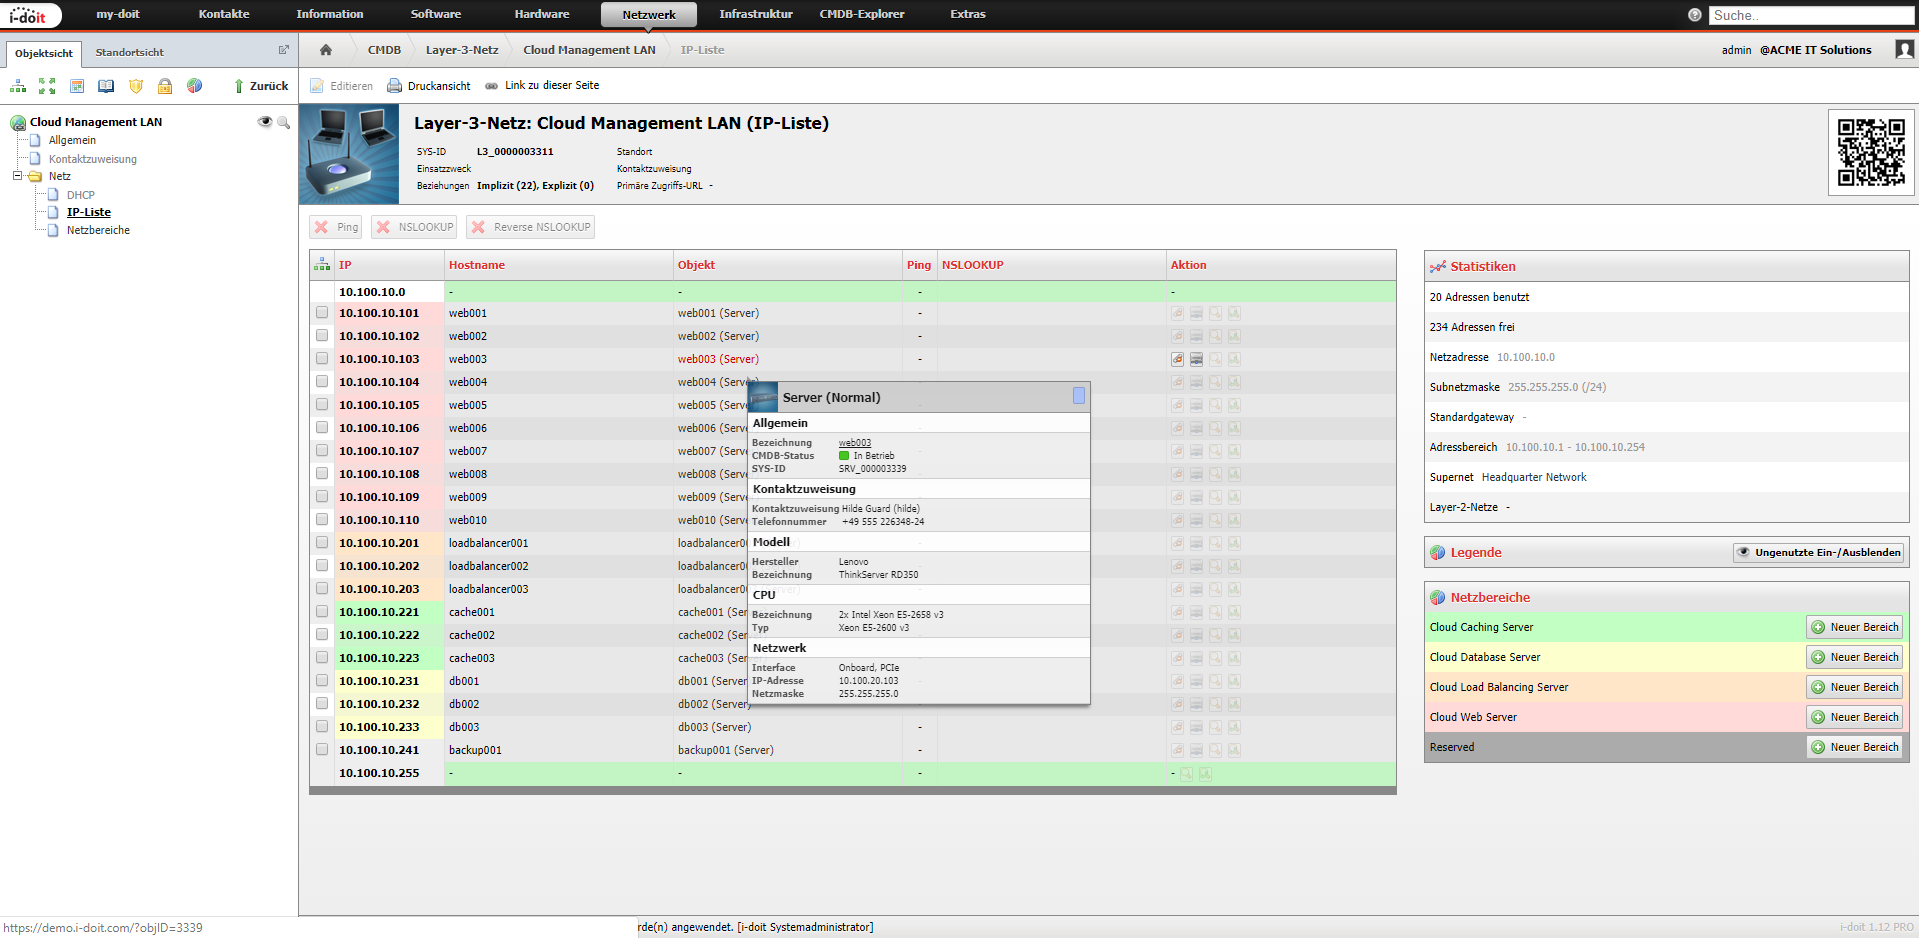
\includegraphics[width=\textwidth]{Anhang/idoitip}
  \quelle[o. \pno]{idoit_2019_idoitip}
  \caption{i-doit IP Management}
\label{fig:idoitip}
\end{figure}

Die \acs{CMDB} wird überwiegend vom Team \textit{Rechenzentrum} über das Webinterface verwendet. Wenn z.~B.~ein neuer Server angefordert wird, erfolgt die Planung von Hostname und IP-Adresse in der \acs{CMDB}.\\
Auch beim Einbau von Hardware, z. B.~neuen Servern, wird die \acs{CMDB} prozessvorbereitend, -begleitend und -unterstützend eingesetzt: Es kann vorab geprüft werden, in welchen Racks noch genug Platz ist und wo entsprechende Möglichkeiten zur Verkabelung von Strom und Netzwerk bestehen. Wenn geprüft wurde, ob Kabel in der benötigten Länge vorrätig sind, kann der Einbau erfolgen und der Status der Hardware wird von \textit{geplant} auf \textit{in Betrieb} geändert.\\
Die verwendeten Kabel werden ebenfalls dokumentiert und die entsprechenden Knotenpunkte (z. B. Netzwerkkartenport zu Switchport oder Netzteil zu Steckerleiste) verknüpft.

Um die \acs{CMDB} von der Kommandozeile aus verwenden zu können, besteht die Möglichkeit, \textit{i-doit-cli} zu nutzen, einen \acf{API}-Client für die i-doit \acs{CMDB}.\\
Mit dem Client lassen sich z. B. Objekte suchen, Details dazu anzeigen und freie IP-Adressen in einem bestimmten Netz anzeigen. Um diese Operationen zu beschleunigen, wird ein lokales Caching verwendet.\\
Außerdem können Dummy Einträge erzeugt werden, um die System-Performance zu testen. Der Client wird bisher nur in einigen Skripten verwendet und hat für die manuellen Tätigkeiten der Mitarbeiter keine Relevanz.
\footcite[Vgl.][o. \pno]{Heisig_2019_idoitcli}

Als Chat-Tool wird derzeit Slack eingesetzt, allerdings ist die Migration nach Cisco WebEx Teams geplant. 


\section{Expertenauswahl}
Um das Experteninterview anwenden zu können, muss geklärt werden, wer als Experte gilt, was Expertenwissen bedeutet und wie man es abruft.\footcite[Vgl.][6\psq]{Bogner_2014_Interview}

\subsection{Kriterien}
Das Wort \textit{Experte} leitet sich aus dem lateinischen \textit{expertus} (erprobt, bewährt) ab, welches wiederum aus dem passiven Verb \textit{experiri} (prüfen, ausprobieren) gebildet wird. Experten sind also Fachleute und Kenner, bzw. allgemein gesprochen Personen, die über ein gewisses Spezialwissen verfügen, das auf der Erfahrung des ausgiebigen Prüfens und Ausprobierens fußt. \footcite[Vgl.][9]{Bogner_2014_Interview}

Gläser und Laudel definieren Experten als Menschen, die ein besonderes Wissen über soziale Sachverhalte besitzen.\footcite[Vgl.][12]{Glaeser_2010_Inhaltsanalyse}\\
Man könnte nun davon ausgehen, dass jeder ein Experte ist, da er sich in seinem Fachgebiet gut auskennt. Genauer betrachtet  gibt es jedoch große Unterschiede zwischen Laien und Experten. Ein solcher Expertenbegriff ist also zu weit gefasst.\footcite[Vgl.][10\psq]{Bogner_2014_Interview}\\
Ein Experte zeichnet sich durch eine bestimmte Kombination von Macht und Wissen aus, welche ihn von Eliten, Spezialisten und spezialisierten Laien unterscheidet. Dieser Zusammenhang ist in  \autoref{fig:experte} erkennbar.\footcite[Vgl.][o. \pno]{Littig_2008}

\begin{figure}[H]
  \centering
  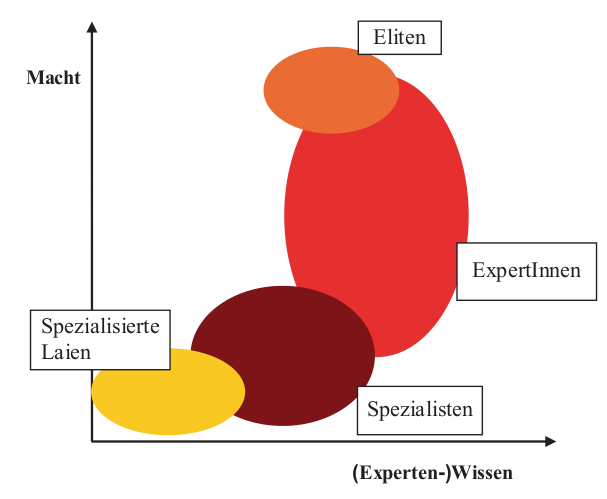
\includegraphics[width=0.8\textwidth]{Anhang/Experte}
  \quelle[o. \pno]{Littig_2008}
  \caption{Experteneinordnung}
\label{fig:experte}
\end{figure}

\glqq{}Der Experte ist -- im Gegensatz zum Spezialisten – nicht allein durch Sonderwissen in Form fachspezifischer Kompetenzen charakterisiert, sondern durch seine Fähigkeit, Verbindungen zu anderen Wissensbeständen und Wissensformen herzustellen und die Relevanz des eigenen Wissens zu reflektieren\grqq
\footcite[][14]{Bogner_2014_Interview}{}.
\footcite[Vgl.][21 \psq]{Hitzler_1994}

Das Interessante am Expertenwissen ist nicht nur das Wissen an sich, sondern die Wirkung in der Praxis. Experten werden gefragt, weil ihre Entscheidungen und Ratschläge das Handeln anderer Akteure mitstrukturieren und -gestalten.\footcite[Vgl.][13]{Bogner_2014_Interview}

Bogner spricht davon, dass Expertenwissen \glqq seine Bedeutung über [...] soziale Wirkmächtigkeit\grqq{}\footcite[][13]{Bogner_2014_Interview} erhält.
Ferner folgert er daraus die Definition:\\ \glqq Experten lassen sich als Personen verstehen, die sich -- ausgehend von einem spezifischen Praxis- oder Erfahrungswissen, das sich auf einen klar begrenzbaren Problemkreis bezieht -- die Möglichkeit geschaffen haben, mit ihren Deutungen das konkrete Handlungsfeld sinnhaft und handlungsleitend für andere zu strukturieren.\grqq{}\footcite[][13]{Bogner_2014_Interview}

Meuser und Nagel betrachten den Experten als Konstrukt des Forschungsinteresses. Die Expertise ist also keine allgemeingültige Eigenschaft oder Fähigkeit einer Person, sondern eine Zuschreibung des Forschenden an diese, im speziellen Kontext der Forschungsfrage. \footcite[Vgl.][181]{Meuser_1994_Interview}

Zusammenfassend lässt sich also sagen, dass Experten über besonderes Wissen auf einem Gebiet verfügen und eine machtvolle Position innehaben können, die zwischen Spezialisten und Eliten liegt. Die Expertise muss nicht durch einen Titel oder Ähnliches verifiziert werden, sie kann auch durch jahrelange berufliche oder private Auseinandersetzung mit einem Thema erlangt werden.

Die Aufgabe des Forschers ist es demzufolge, die Experten für seine spezielle Forschungsfrage ausfindig zu machen und zu befragen.

Im Falle dieser Arbeit stammen die Experten aus dem beruflichen Umfeld des Autors und haben sich durch wichtige Positionen oder herausragende Leistungen auf dem Gebiet des Forschungsthemas hervorgetan.



\subsection{Vorstellung}
Als Experten zur Befragung wurden die \acs{IVZ} Mitarbeiter Alexander Hemmerich und Jörg Middendorf, sowie die synetics Mitarbeiter Konrad Buck und Daniel Kirsten ausgewählt.

Hemmerich und Middendorf sind seit 2011 Teil der \acs{IVZ} Belegschaft und können daher aus einiger Erfahrung schöpfen. Hemmerich ist aktuell Leiter des Rechenzentrums am Standort Köln mit den Tätigkeitsschwerpunkten Storage, Backup und Loadbalancer. Somit hat er einen guten Gesamtüberblick über die Tätigkeiten des Rechenzentrums.\\
Middendorf ist neben der Unix- und Storage Administration auch für die \acs{CMDB} des \acs{IVZ} zuständig und hat somit ein umfangreiches Wissen über Infrastruktur, Aufbau, Funktionen und Schnittstellen der \acs{CMDB}.

Buck ist PR- und Community-Manager sowie Kommunikationsberater der synetics GmbH für das Produkt i-doit. Er hat  Publizistik und Germanistik studiert und sich als IT-Fachjournalist fortgebildet. Für synetics übernimmt er die Moderation und Kundenkommunikation, um für dauerhafte Kundenbindung zu sorgen. Durch seine Tätigkeiten hat er ein gutes Gesamtbild der Unternehmen, die eine i-doit \acs{CMDB} des Herstellers synetics einsetzen und kann den Nutzen von ChatOps für diese beurteilen. 
\footcites[Vgl.][o. \pno]{Buck_2018_Allgemein}[Vgl.][o. \pno]{Buck_2018_Referenzen}

Kirsten arbeitet seit 1998 bei der synetics GmbH und ist Produktmanager für die i-doit \acs{CMDB}. Zuvor war er als IT-Berater im Bereich Infrastruktur und Server tätig und konnte Erfahrung zu den Themen Routing/Switching, virtuelle Umgebungen und Speichernetze sammeln.
\footcite[Vgl.][o. \pno]{Kirsten_2017}

Die Experten selbst haben nicht direkt mit Chatbots zu tun, sondern sollen sie in ihrem beruflichen Kontext, auf dem sie Experten sind, also Rechenzentrumsbetrieb und \acs{CMDB}, bewerten.\\
Durch die genannten Experten werden wichtige Schlüsselfunktionen betrachtet und deren Perspektiven berücksichtigt. Auf normale \textit{Verwender} der \acs{CMDB} kann daher als Interviewpartner verzichtet werden.


\section{Ermittlung der Anforderungen an einen CMDB Chatbot}
Die Ermittlung der Anforderungen ist der erste Schritt des Anforderungsmanagements. Im Experteninterview werden darunter die ersten beiden Schritte \textit{Leitfadenerstellung} und \textit{Tonaufnahme} verstanden.

Bei der Ermittlung der Anforderungen können verschiedene Quellen, wie z. B. Stakeholder, Dokumente oder aktive Systeme genutzt werden, um Anforderungen zu detektieren und zu verfeinern.\footcite[Vgl.][21]{Pohl_2015_Requirements}

Das Interview ist eine mögliche Befragungstechnik, bei der ein Stakeholder (Interviewpartner) vom Requirements Engineer (Interviewer) vorgegebene Fragen gestellt bekommt. Die Antworten werden protokolliert. Etwaige Rückfragen können sofort im Gesprächsverlauf geklärt werden. Durch geschickt gestellte Fragen können auch unterbewusste Anforderungen ermittelt werden. Der Verlauf des Gesprächs kann individuell angepasst werden, es wird gezielt nachgefragt und auf einzelne Themen eingegangen, um das behandelte Thema möglichst komplett abzubilden.\footcite[Vgl.][28]{Pohl_2015_Requirements}

\subsection{Leitfadenerstellung}
Der Einsatz eines Leitfadens dient dazu, das Interview thematisch zu begrenzen und würdigt den Expertenstatus durch die damit verbundene Auseinandersetzung mit dem Thema. Der Leitfaden ist dabei nicht strikt zu befolgen, sondern bietet lediglich das Grundgerüst des Interviews. Reihenfolge und Tiefe der Fragen bzw. Themenkomplexe können zwischen den Interviews variieren. Die Fragen sollten dabei nicht abgelesen werden, sondern in der \glqq{}Sprache des Experten\grqq
\footcite[][449]{Meuser_1991_Interview}
gestellt werden.
\footcite[Vgl.][448\psq]{Meuser_1991_Interview}

Leitfäden in der qualitativen Forschung liegen in Art und Umfang in verschiedensten Ausprägungen vor. Je nach Forschungs- und Interviewstil reichen sie von groben Themensammlungen bis hin zu ausführlichen Leitfäden mit ausformulierten Fragen.\\
Ein Leitfaden besteht aus verschiedenen Themenblöcken, mit darin enthaltenen Hauptfragen, die sich weiter in Teilaspekte aufgliedern können. Die Hauptfragen sollten bei dem Interview auf jeden Fall zur Sprache kommen und die Teilaspekte können angesprochen werden, um die Frage zu vertiefen.
\footcite[Vgl.][27\psq]{Bogner_2014_Interview}

Der allgemeingültige Leitfaden für alle in dieser Untersuchung zu Wort kommenden Experten ist in \autoref{Leitfaden} zu finden. Er gliedert das Thema in die drei Themenkomplexe \textit{CMDB im Rechenzentrum}, \textit{Chatbots allgemein} und \textit{Chatbots zur Bedienung der CMDB}.

\subsection{Tonaufnahme}
Die Interviews mit Alexander Hemmerich und Jörg Middendorf wurden persönlich durchgeführt und mit der Audiorekorderfunktion eines Handys aufgezeichnet. Die Interviews mit Daniel Kirsten und Konrad Buck erfolgten in dem Konferenztool Cisco WebEx Meeting und wurden mit dessen Aufnahmefunktion aufgezeichnet.



\section{Dokumentation der Anforderungen}
Die Dokumentation der Anforderungen ist der zweite Schritt des Anforderungsmanagements. Im Experteninterview werden darunter die Schritte drei bis fünf, \textit{Transkription}, \textit{Paraphrase} und \textit{(Bildung von) Überschriften} verstanden und es ist das einzelne Interview im Fokus.

Die erarbeiteten Anforderungen werden in natürlicher Sprache oder in dafür vorgesehenen Modellen dokumentiert, wobei entsprechende Techniken zum Einsatz kommen. \footcite[Vgl.][4]{Pohl_2015_Requirements}

Die im Requirements Engineering anfallenden Tätigkeiten müssen geeignet dokumentiert werden. Dazu zählt z. B.~auch die Erstellung von Interviewprotokollen. Als Dokumentation gilt jede Form der formalen Darstellung, von Beschreibung in natürlicher Sprache über strukturierten Text bis hin zu formalen Techniken wie Diagrammen. Die Dokumentationsform sollte der zugrunde liegenden Aktivität angemessen sein und diese sinnvoll wiedergeben. \footcite[Vgl.][35\psqq]{Pohl_2015_Requirements}


\subsection{Transkription}
Das Hauptaugenmerk von Experteninterviews liegt auf der Gewinnung von Wissen. Daher ist eine mühselige Notation, wie sie bei narrativen Interviews vorgenommen wird nicht nötig. Elemente wie Pausen, Betonung oder Stimmlage werden nicht interpretiert.
Eine Transkription wird in der Regel nicht für die gesamte Tonaufnahme durchgeführt, sondern kann selektiv erfolgen. Bei der Abfrage von Betriebswissen fällt die Transkription umfangreicher aus als bei Kontextwissen. \footcite[Vgl.][455\psq]{Meuser_1991_Interview}

Zur Transkription wurden die Audioaufnahmen unter Linux mit \acf{MPD} wiedergegeben und mit dem \acf{MPC} gesteuert. Dieser erlaubt die Bedienung des Backends mit Kommandozeilenbefehlen. So lassen sich globale Tastaturkürzel festlegen, um die Wiedergabe zu pausieren oder einige Sekunden zurückzuspringen und diese können genutzt werden, um die Wiedergabe zu steuern, ohne den Editor zu verlassen oder die Hände von der Tastatur zu heben.

Die Transkripte der Interviews sind in \autoref{Interview_Hemmerich}, \autoref{Interview_Middendorf}, \autoref{Interview_Kirsten} und \autoref{Interview_Buck} zu finden.


\subsection{Paraphrase}
Die Paraphrase erfolgt unter Berücksichtigung der Forschungsfrage und gibt die Aussagen der Experten chronologisch geordnet und unverfälscht wieder, wobei diese zu thematischen Verbünden zusammengefasst werden. Ob die Passage zusammenfassend oder detailliert wiedergegeben wird, hängt von der Priorität des Themas und nicht zwangsläufig von der ihm gewidmeten Zeit ab.
\footcite[Vgl.][456\psq]{Meuser_1991_Interview}

In den folgenden Abschnitten werden die einzelnen Interviews paraphrasiert. Dabei werden die in \autoref{ueber} vorgesehenen Überschriften der besseren Lesbarkeit halber bereits der Passage vorangestellt.

\subsubsection{Interview Hemmerich}
\textbf{\acs{CMDB} allgemein: }Es soll zunächst das Interview mit Alexander Hemmerich betrachtet werden. Er beschreibt die \acs{CMDB} als Tool, um \glqq{}Configuration Items im Rechenzentrum, vom Kabel über Server über Ausstattung innerhalb eines Rechnerraums\grqq
\footcite[][o. \pno]{Hemm_2019}
zu verwalten und zählt auch die vermerkten Lizenzen und Supportverträge dazu.\\
Seiner Meinung nach lässt sich die Vielzahl an Komponenten \glqq{}gar nicht mehr anders handhaben\grqq
\footcite[][o. \pno]{Hemm_2019}.
Außerdem führt er an, dass die \acs{CMDB} gefordert sei, um eine ISO 27001 Zertifizierung zu erlangen.
\footcite[Vgl.][o. \pno]{Hemm_2019}

\textbf{Bestandsprüfung, Statusabfrage, Ressourcenübersicht: }Bei der täglichen Arbeit nutzt Hemmerich die \acs{CMDB} \glqq{}[u]m Gegenstände und Bestände abzufragen\grqq
\footcite[][o. \pno]{Hemm_2019}
, also beispielsweise zur Prüfung des aktuellen Kabelbestands im Lager oder um den Status eines Servers abzufragen (eingelagert, verschrottet, etc.).\\
Außerdem nutzt er die Report Funktion, um zu ermitteln, welche Ressourcen ein Kunde oder eine Anwendung belegt (RAM, CPU, etc.). Dies sei einerseits bei der Abrechnung ausschlaggebend und andererseits bei der Beantragung neuer Dienstleistungen, wie \glqq{}zusätzliche[n] virtuelle[n] Maschinen\grqq
\footcite[][o. \pno]{Hemm_2019}
,nötig, um festzustellen, ob die Anforderungen durch den bestehenden Vertrag abgebildet sind oder ob eine Erweiterung erfolgen muss. \glqq{}[D]as \ldots [geht] \ldots zu unserem Vertrieb und daraus entsteht \ldots eine Preisinformation für den Kunden\grqq
\footcite[][o. \pno]{Hemm_2019}.{}
\footcite[Vgl.][o. \pno]{Hemm_2019}

\textbf{\acs{CMDB} Schnittstellen: }Hemmerich hält die \acs{CMDB} für besonders wichtig, da sie \glqq{}das führende System ist\grqq
\footcite[][o. \pno]{Hemm_2019}
. Das Monitoring System und ein Scan System liefern Daten zu und diese werden in der CMDB \glqq{}aggregiert, um eine Gesamtsicht auf das Rechenzentrum, auf die Ausstattung und sogar auf die Standorte des Unternehmens zu bieten.\grqq
\footcite[][o. \pno]{Hemm_2019}
.\\
Außerdem ergänzt er, dass neben Configuration Items des Rechenzentrums auch Gebäude, Büros und Mitarbeiter in der \acs{CMDB} vermerkt sind.
\footcite[Vgl.][o. \pno]{Hemm_2019}

\textbf{Chatbots allgemein: }Als Chatbots betrachtet Hemmerich Bots, \glqq{}mit denen man kommunizieren kann\grqq
\footcite[][o. \pno]{Hemm_2019}
und die auf Anfrage \glqq{}Informationen liefern\grqq
\footcite[][o. \pno]{Hemm_2019}
oder \glqq{}Aktion[en] ausführen\grqq
\footcite[][o. \pno]{Hemm_2019}
. Persönlich hat er noch keine Erfahrungen mit Chatbots oder ChatOps gemacht, er blickt jedoch gespannt auf deren großes Einsatzspektrum.
\footcite[Vgl.][o. \pno]{Hemm_2019}

\textbf{Chatbots zur Automatisierung: }Als Ersatz für menschliche Arbeitskräfte betrachtet Hemmerich Chatbots nicht, sondern vielmehr als Unterstützung bei der täglichen Arbeit. \glqq{}Ein Chatbot könnte einfache Tätigkeiten übernehmen und zur Automatisierung des täglichen Rechenzentrumsbetriebs beitragen.\grqq
\footcite[][o. \pno]{Hemm_2019}
Aus seiner Sicht können dadurch alltägliche Arbeitsschritte vereinfacht werden.
\footcite[Vgl.][o. \pno]{Hemm_2019}

\textbf{Suchfunktion, nächste freie IP, Serverplanung, Schnittstellenanbindung: }Als mögliche Funktionen für einen Chatbot, der die \acs{CMDB} bedient, kann Hemmerich sich die Suche nach Objekten und die Anzeige der nächsten freien IP-Adresse in einem bestimmten Netz vorstellen.
Dabei hat er einen Workflow vor Augen, bei dem ein Server über den Bot geplant und mit einem Namen versehen wird. Daraufhin soll für diesen eine freie IP-Adresse in einem bestimmten Netz gesucht und reserviert werden.\\
Als sinnvolle Ergänzung würde er hier begrüßen, dass in diesem Workflow direkt die virtuelle Maschine bereitgestellt, die Konfiguration per Puppet vorgenommen und die Netzkonfiguration hergestellt wird. Davon verspricht er sich eine Vermeidung von Inkonsistenzen zwischen CMDB und Realität. 
\footcite[Vgl.][o. \pno]{Hemm_2019}\\
Dies übersteigt den \acs{CMDB}-Fokus, kann jedoch im Ausblick und in der Möglichkeit einer Anbindung von weiteren Tools und Schnittstellen berücksichtigt werden.

\textbf{Vermeidung Fehlbedienung, Berechtigungskonzept, Nachvollziehbarkeit: }Die Integrität der \acs{CMDB} ist für Hemmerich ein hohes Gut und eine versehentliche Löschung oder Manipulation von Daten durch \glqq{}Fehlfunktion oder Fehlbedienung [des] Bots\grqq
\footcite[][o. \pno]{Hemm_2019}
sollte vermieden werden. Bei der Entwicklung sollte darauf geachtet werden, die Betriebssicherheit zu gewährleisten.\\
Außerdem legt Hemmerich Wert darauf, dass nur ein bestimmter Personenkreis berechtigt ist, Änderungen oder Löschungen vorzunehmen und es soll nachvollziehbar sein, wer Änderungen vorgenommen hat.
\footcite[Vgl.][o. \pno]{Hemm_2019}

\textbf{Akzeptanz, Webinterface Eingaben: }Probleme erwartet Hemmerich bei der Einführung eines \acs{CMDB} Chatbots nicht, er könnte sich jedoch vorstellen, dass ältere Kollegen etwas Zeit brauchen, um sich daran zu gewöhnen und lieber weiterhin die Eingaben über das Webinterface vornehmen. 
Da es sich aber größtenteils um junge, motivierte Menschen handelt, \glqq{}die auch in der Freizeit viel mit neuen Technologien arbeiten\grqq
\footcite[][o. \pno]{Hemm_2019}
, erwartet Hemmerich, dass ein \acs{CMDB} Chatbot \glqq{}in dem Bereich sehr großen Anklang finden wird\grqq
\footcite[][o. \pno]{Hemm_2019}{}.
\footcite[Vgl.][o. \pno]{Hemm_2019}

\textbf{Transparenz, Arbeitsüberwachung: }Die ChatOps-inhärente Transparenz befürwortet Hemmerich grundsätzlich. Er gibt jedoch zu bedenken, dass man darin eine Form von Arbeitsüberwachung sehen kann. In einem transparenten Chat Raum sei es denkbar, dass man nachvollziehen kann, woran und wie intensiv andere Kollegen arbeiten, deshalb solle man diesbezüglich Rücksprache mit dem Betriebsrat halten.\\
Seitens der Kollegen rechnet er mit Zustimmung und Offenheit für diese Arbeitsweise. 
\footcite[Vgl.][o. \pno]{Hemm_2019}

\textbf{Framework Python, Weiterentwicklung: }Bei der Wahl des Bot-Frameworks legt Hemmerich Wert auf die Wartbarkeit und Möglichkeit der Weiterentwicklung. Aufgrund des fundierten Python Know-hows im Rechenzentrum würde er einen Bot in dieser Sprache bevorzugen. Er empfiehlt, \glqq{}Entwicklungen in den Sprachen zu betreiben, wo das Know-how da ist und auch in Zukunft da sein wird. Denn es gibt nichts Schlimmeres als eine Anwendung, die ein Praktikant oder Azubi entwickelt hat in einer Sprache, mit der sich hier keiner auskennt und die nach seinem Weggang eben nicht mehr wartbar ist.\grqq
\footcites[][o. \pno]{Hemm_2019}[Vgl.][o. \pno]{Hemm_2019}

\textbf{Charakter, Avatar: }Bei der Modellierung der Persönlichkeit des \acs{CMDB} Chatbots verweist Hemmerich auf die Professionalität des Rechenzentrumsbetriebs und schlägt einen dementsprechenden Charakter vor. Da das Unternehmen im Medienbereich tätig ist, könnte er sich Maus oder Elefant aus der Sendung mit der Maus als Avatar vorstellen. Da im Alltag eine humorvolle Stimmung herrscht, würde er einen solchen Charakterzug befürworten.  
\footcite[Vgl.][o. \pno]{Hemm_2019}

\textbf{Betriebssicherheit: }\glqq{}[I]m Hinblick auf die Betriebssicherheit\grqq
\footcite[][o. \pno]{Hemm_2019}
zieht Hemmerich einen regelbasierten Chatbot einem KI-gestützten vor, da das Regelwerk klar definiert werden kann und keine ungeplanten oder unbeabsichtigten Aktionen ausgeführt werden, die im schlimmsten Fall zu \glqq{}einer Katastrophe oder Störung\grqq 
\footcite[][o. \pno]{Hemm_2019}
 führen können. 
\footcite[Vgl.][o. \pno]{Hemm_2019}

\textbf{Potenzial: }Auch für andere Tätigkeiten des Rechenzentrums sieht Hemmerich \glqq{}großes Potenzial\grqq
\footcite[][o. \pno]{Hemm_2019}
 in der Verwendung von ChatOps.
 Er warnt davor, sich vor einer solchen Technologie zu fürchten und sie als Bedrohung des eigenen Arbeitsplatzes zu sehen. Stattdessen sei sie eine \glqq{}sinnvolle Ergänzung der täglichen Arbeit\grqq
\footcite[][o. \pno]{Hemm_2019}
. Auch für andere Unternehmen kann er sich eine ChatOps Lösung vorstellen. \glqq{}Jeder der eine CMDB einsetzt, kann von so etwas nur profitieren.\grqq
\footcites[][o. \pno]{Hemm_2019}[Vgl.][o. \pno]{Hemm_2019}



\subsubsection{Interview Middendorf}
\textbf{CMDB allgemein: }Als Nächstes soll das Interview mit Jörg Middendorf betrachtet werden. Unter einer \acs{CMDB} versteht er eine Datenbank, in der \glqq{}alle Gerätschaften eines Unternehmens dokumentiert sind und in Relation gesetzt werden\grqq.
\footcite[][o. \pno]{Midd_2019}
.
Z. B.~werden \glqq{}Server, Lizenzen und Aufstellungsorte\grqq
\footcite[][o. \pno]{Midd_2019}
 dokumentiert, um sie für Supportfälle oder Planungstätigkeiten zu nutzen.
\footcite[Vgl.][o. \pno]{Midd_2019}

\textbf{Suchfunktion, Standortabfrage, Standortreport: }Bei der täglichen Arbeit nutzt Middendorf die \acs{CMDB} vor allem zur \glqq{}Dokumentation neu erstellter Maschinen\grqq
\footcite[][o. \pno]{Midd_2019}
 und um Objekte wie Server zu suchen und deren Standort zu überprüfen. Außerdem nutzt er die Reporting Funktion zur Unterstützung bei Planungen, z. B.~um festzustellen, \glqq{}wie viele Server an einem Standort \ldots sind\grqq
\footcite[][o. \pno]{Midd_2019}
. Durch ein aktuelles \glqq{}Projekt, bei dem Rechenzentren umgezogen werden\grqq
\footcite[][o. \pno]{Midd_2019}
 wird diese Funktionalität häufig benötigt. Abseits davon nutzt er die \acs{CMDB} um IP-Netze zu dokumentieren und neue Adressen zu vergeben bzw. nachzuprüfen, wofür bestehende genutzt werden.
\footcite[Vgl.][o. \pno]{Midd_2019}

\textbf{CMDB Schnittstellen: }Besonders wichtig findet Middendorf die Schnittstellen der \acs{CMDB}. Es gibt einerseits die Möglichkeit, aus dem Monitoring Daten abzufragen und andererseits die Möglichkeit, in \glqq{}der CMDB geplante Daten ins Monitoring zu transferieren\grqq
\footcite[][o. \pno]{Midd_2019}
.
Außerdem findet er die Reporting-Funktion für die tägliche Arbeit sehr wichtig.
\footcite[Vgl.][o. \pno]{Midd_2019}

\textbf{ChatOps allgemein: }ChatOps versteht Middendorf im DevOps-Gedanken, also als Zusammenarbeit von Entwicklern und Administratoren.
Mit Chatbots hatte er vor allem schon bei Supportanbietern zu tun, die diese einsetzen, um \glqq{}Anliegen aufzunehmen und zu klassifizieren\grqq
\footcite[][o. \pno]{Midd_2019}
.
Auch mit Sprachassistenten, wie Siri oder Alexa hatte er bereits zu tun.
\footcite[Vgl.][o. \pno]{Midd_2019}

\textbf{Softwarestand, IP-Adresse, Automatisierung: }Im Rechenzentrumsbereich sieht Middendorf für Chatbots vor allem Potenzial, Standardaufgaben zu übernehmen. Dazu zählt er die Suche nach dem Standort von Geräten und die Ermittlung von Softwareständen und IP-Adressen. Für diese Aufgaben werden bisher die RZ-Mitarbeiter persönlich oder per E-Mail gefragt. Von einer Automatisierung per Chatbot verspricht er sich für die Mitarbeiter eine Konzentration auf die eigentlichen Aufgaben des RZ-Betriebs.
\footcite[Vgl.][o. \pno]{Midd_2019}

\textbf{Mobilität, IP-Adresse, Netzinformationen, Ressourcen: }Als Vorteil eines Chatbots zur Bedienung der \acs{CMDB} sieht Middendorf vor allem die Mobilität. Als konkretes Beispiel könne er sich hier vorstellen, bereits auf dem Weg zum Rechenzentrum nach einem Server zu suchen, um herausfinden, in welchem Rack und an welcher Position sich dieser befindet. Außerdem könne er vor Ort prüfen, welche Software der Maschine zugewiesen ist, welche IP sie hat, welchem Subnetz und VLAN sie angehört und wie viel Festplattenplatz und RAM belegt sind.
Außerdem ergänzt er, dass die Abfrage per Webinterface auf Mobilgeräten möglicherweise gar nicht möglich sei.
\footcite[Vgl.][o. \pno]{Midd_2019}

\textbf{Servereinbau, Serverausbau: }Als Möglichkeit zur Arbeitsvereinfachung sieht Middendorf einen \acs{CMDB} Chatbot auch beim Einbau von neuer Hardware im Rechenzentrum. So könne er direkt den Einbauort vermerken, den Server benennen und ihm eine IP-Adresse zuweisen. Beim Ausbau eines Geräts könne er hingegen den Status des Geräts auf \textit{außer Betrieb} oder \textit{verschrottet} setzen.
\footcite[Vgl.][o. \pno]{Midd_2019}

\textbf{Berechtigungskonzept, API Einsatz: }Nach Middendorfs Ansicht sollte nur ein bestimmter Personenkreis Zugriff auf die \acs{CMDB} Features haben. Dies gelte vor allem für die schreibenden Funktionen, für die lesenden sei eine andere Regelung denkbar (z. B. Öffnung der Suche für alle).
Als weitere Anforderung gibt er vor, die \acsp{API} oder Command Line Tools des \acs{CMDB} Herstellers zu nutzen und nicht direkt auf die Datenbank zuzugreifen.
\footcite[Vgl.][o. \pno]{Midd_2019}

\textbf{Nachvollziehbarkeit: }Middendorf ergänzt weiterhin, dass nachvollziehbar sein sollte, wer welche Änderung vorgenommen hat. Dies könne beispielsweise im Chatverlauf oder in einem Log File festgehalten werden und solle dauerhaft abrufbar sein. Im Idealfall werde diese Information direkt bei der Manipulation eines \acs{CI}s als Kommentar vermerkt.
\footcite[Vgl.][o. \pno]{Midd_2019}

\textbf{Arbeitsüberwachung: }Mit Problemen beim Einsatz eines \acs{CMDB} Chatbots rechnet Middendorf grundsätzlich nicht, er gibt jedoch zu bedenken, dass eine Chat Software, die außerhalb eines Unternehmens gehostet wird und Unternehmensinterna darin kommuniziert werden, besondere Regularien erfüllen müsse. Die Transparenz, die mit ChatOps einhergeht, sieht Middendorf als Vorteil. Man könne direkt mitverfolgen, was sich in der Umgebung ändert oder sich nach Abwesenheit einen Überblick über die erfolgten Änderungen verschaffen. Allerdings solle diese Übersicht nicht zur Auswertung der Arbeitsleistung herangezogen werden.
\footcite[Vgl.][o. \pno]{Midd_2019}

\textbf{Framework: }Bei der Wahl des Bot-Frameworks sieht Middendorf Errbot in Betrachtung der Weiterentwicklung als klaren Favoriten, da im Rechenzentrum bereits großes Python Know-how vorhanden und die Sprache auch für Laien recht leicht lesbar ist.
\footcite[Vgl.][o. \pno]{Midd_2019}

\textbf{Charakter: }Als Persönlichkeit für einen Chatbot kann sich Middendorf keine konkrete Figur oder Person vorstellen. Er würde jedoch einen humorvollen Charakter bevorzugen. Es müsse aber darauf geachtet werden, dass die Aussagen des Bots nicht verletzend wirken. Bei mehrfachen Anfragen nach dem gleichen Inhalt oder Falscheingaben könne durchaus eine freche Antwort folgen. 
\footcite[Vgl.][o. \pno]{Midd_2019}

\textbf{Ansatz, Hilfe: } Bei der Wahl der Art des Chatbots spricht sich Middendorf klar für einen regelbasierten Ansatz aus. Der Bot solle nur genau das machen, was angefordert ist und nichts, das er durch künstliche Intelligenz dazu gelernt hat. Eine Interpretation solle nicht erfolgen, das Ergebnis könne dann zu stark von der Erwartung abweichen. Ein KI-gestützter Chatbot sei deshalb höchstens für andere Anwendungen, wie die Begrüßung neuer Mitarbeiter oder die Beantwortung der FAQ zu bevorzugen, nicht aber für Rechenzentrumstätigkeiten.\\
Da die RZ Mitarbeiter täglich auf Kommandozeilenebene arbeiten geht Middendorf davon aus, dass sie mit den Befehlen des Bots schnell zurechtkommen. Außerdem müsse dieser über eine Hilfe Funktion verfügen, welche die gültigen Kommandos mit Beispielen ausgibt.  Eine Einführungsveranstaltung solle vor Inbetriebnahme des Bots erfolgen.
\footcite[Vgl.][o. \pno]{Midd_2019}

\textbf{Nachfrage, Herstellerkonsolidierung: } Bei kritischen Aktionen hält Middendorf eine zusätzliche Abfrage für sinnvoll. Außerdem sei es bisher der Fall, dass der gleiche Hersteller unter unterschiedlichen Namen im System vermerkt ist (z. B. HP, Hewlett-Packard). Daher sei es sinnvoll, bei der Eintragung neuer Hardware, die bestehenden Hersteller zu berücksichtigen und bei Ähnlichkeit vorzuschlagen, um Dopplungen zu vermeiden. Dies solle interaktiv erfolgen.
\footcite[Vgl.][o. \pno]{Midd_2019}

\textbf{Potenzial: } Für andere Rechenzentrumstätigkeiten sieht Middendorf ebenfalls Potenzial. Alle Dienste mit einer API seien zur Automatisierung gut geeignet. Er könne sich z. B.~die Provisionierung von virtuellen Maschinen, die Anbindung an Puppet und die Bearbeitung von DNS Einträgen vorstellen. Auch für andere Unternehmen hält er ChatOps für sinnvoll. Vor allem die Knappheit an qualifiziertem Personal spreche für mehr Automatisierung und ein Chatbot sei dafür eine sinnvolle Möglichkeit, da er bei der täglichen Arbeit die Komplexität von Workflows reduziert.
\footcite[Vgl.][o. \pno]{Midd_2019}



\subsubsection{Interview Kirsten}
\textbf{CMDB allgemein: }Als Nächstes soll das Interview mit Daniel Kirsten betrachtet werden. Er betrachtet in seiner Funktion als Produktmanager die \acs{CMDB} streng nach \acs{ITIL} und versteht darunter die zentrale Erfassung von IT-Infrastruktur Elementen und deren Konfiguration. Das Verständnis unterscheide sich dabei stark und die gespeicherten Daten reichten von Asset Management Informationen bis hin zu technischen Konfigurationen. Außerdem spreche man nach \acs{ITIL} nicht mehr von einer \acs{CMDB}, sondern eher von einem \acf{CMS}, welches eine Vereinigung mehrerer \acsp{CMDB} darstellt. Der Großteil der Anwender betrachte die \acs{CMDB} als Datenbank, die \glqq{}alle Komponenten einer IT-Infrastruktur vereint, dokumentiert und im Idealfall mindestens die technischen Grundkonfigurationen dieser Elemente aufnimmt.\grqq 
\footcites[][o. \pno]{Kirsten_2019}[Vgl.][o. \pno]{Kirsten_2019}

\textbf{Interner Einsatz: }Bei der täglichen Arbeit nutzt Kirsten selbst die i-doit \acs{CMDB}, um die internen technischen Komponenten zu dokumentieren. Sie diene als Nachschlagewerk und werde manuell, ohne Zuhilfenahme automatisierter Prozesse befüllt. Neben den internen Komponenten seien auch noch Cloud Ressourcen dort dokumentiert. 
\footcite[Vgl.][o. \pno]{Kirsten_2019}

\textbf{IP-Adressen, Passwörter, Cloud: }Die Erfassung von IP-Adressen und Passwörtern in der \acs{CMDB} findet Kirsten besonders wichtig. Da vermehrt Cloud Lösungen eingesetzt werden, sei es zudem wichtig, Zugang und verknüpfte Dienste zu diesen Ressourcen zu dokumentieren.
\footcite[Vgl.][o. \pno]{Kirsten_2019}

\textbf{ChatOps, Chatbots, Output: }Mit ChatOps hatte Kirsten noch keine Berührungspunkte, im Grunde verstehe er es aber als DevOps Prozess, der durch Chatbots unterstützt wird.  Beim Thema Chatbots kann er aus einiger Erfahrung schöpfen, da er fast zehn Jahre lang TCL Skripte für Eggdrop Bots programmierte. Einen Chatbot definiert er als Instanz, die User Input entgegennimmt, verschiedene Datenquellen nutzt und einen menschenlesbaren Output liefert.
\footcite[Vgl.][o. \pno]{Kirsten_2019}

\textbf{Vorteile Chatbots: }Als Vorteil von Chatbots sieht Kirsten den schnellen Abruf von Informationen. Damit spare man sich z. B.~das Öffnen des Browsers und die Anmeldung. Er warnt jedoch auch davor, zu viele Informationen von einem Chatbot ausgeben zu lassen. Für die gängigsten Funktionen einer \acs{CMDB} kann Kirsten sich einen Chatbot gut vorstellen. 
\footcite[Vgl.][o. \pno]{Kirsten_2019}

\textbf{IP-Adressen, Standortdaten, Kontaktpersonen, Suche, Logbuch: }Da der Output von Chatbots auf Text limitiert ist, empfiehlt Kirsten, die Prozesse eines Chatbots nicht zu komplex zu gestalten. Als konkrete Anwendungsfälle eines \acs{CMDB} Chatbots könne er sich die Abfrage von IP-Adressen, Standortdaten oder Kontaktpersonen vorstellen. Außerdem sei eine Suche sinnvoll, wenn man den kompletten Objektnamen nicht weiß. Zudem könne er sich vorstellen, freie IP-Adressen zu reservieren oder als Administrator Änderungen am Logbuch zu erfassen. Vor allem die Ausgabe von Informationen hält Kirsten für leicht umsetzbar, die Eingabe stehe eher im Hintergrund, da die Normalisierung fehleranfällig ist.
\footcite[Vgl.][o. \pno]{Kirsten_2019}

\textbf{Rechtesystem, Plattform-Agnostik: }Ein \acs{CMDB} Chatbot soll laut Kirsten ein Rechtesystem abbilden, das nur den Nutzern Informationen darstellt, die berechtigt sind, diese zu sehen. Er sehe sonst ein Missbrauchspotenzial. Außerdem rät er dazu, einen Chatbot nur im internen Netz zu betreiben, um die \acs{CMDB} nicht für das Internet zugänglich zu machen. Weiterhin rät er dazu, den Chatbot möglichst plattform-agnostisch zu gestalten, also die Möglichkeit zu bieten, \glqq{}verschiedene Chatsysteme daran anzubinden\grqq
\footcite[][o. \pno]{Kirsten_2019}
. Als Standard sehe er jedoch aktuell Slack.
\footcite[Vgl.][o. \pno]{Kirsten_2019}

\textbf{Akzeptanz, Feedback: }Mit Problemen bei der Akzeptanz eines \acs{CMDB} Chatbots rechnet Kirsten nicht. Es müsse einer die Funktionen in einem öffentlichen Raum nutzen, damit andere das Potenzial erkennen und es ihm gleich tun. So könne Viralität entstehen. Man erhalte als Entwickler jedoch kaum Feedback. Wenn der Bot nicht angenommen wird, spiegele es sich lediglich darin, dass er nicht genutzt wird. Generell ist Kirsten jedoch zuversichtlich bezüglich der Akzeptanz eines \acs{CMDB} Chatbots.
\footcite[Vgl.][o. \pno]{Kirsten_2019}

\textbf{Programmiersprache: }Wegen der großen Verbreitung, der Mächtigkeit und dem langen Bestehen, empfiehlt Kirsten als Programmiersprache Python. Bei neueren Technologien wie Ruby oder Coffeescript rate er eher zur Vorsicht. 
\footcite[Vgl.][o. \pno]{Kirsten_2019}

\textbf{Persönlichkeit, Avatar: }Dem CMDB Chatbot eine Persönlichkeit zu verleihen hält Kirsten nicht für notwendig. Da vorwiegend Techniker damit arbeiten sollen, seien Formalitäten wie Begrüßungen überflüssig. Als Avatar könne er sich jedoch einen Roboter vorstellen. 
\footcite[Vgl.][o. \pno]{Kirsten_2019}

\textbf{Ansatz: }Kirsten spricht sich für einen regelbasierten Chatbot aus, ein KI-gestützter Bot sei eher schwierig und führe zu Frustrationen beim Anlernen. Er empfiehlt die Konzentration auf \glqq{}kleine, regelbasierte Aufgaben\grqq
\footcite[][o. \pno]{Kirsten_2019}.{}
\footcite[Vgl.][o. \pno]{Kirsten_2019}

\textbf{Potenzial: }Für andere Unternehmen sieht Kirsten großes Potenzial für die Verwendung eines \acs{CMDB} Chatbots. Vor allem durch die Verwendung von Slack und WhatsApp seien die Anwender mit dem Medium vertraut und können damit professionell umgehen. Schnittstellen dazu zu haben, halte er daher für sinnvoll.
\footcite[Vgl.][o. \pno]{Kirsten_2019}

\textbf{Reaktivität: }Ergänzend warnt Kirsten davor, Funktionen zu nutzen, die automatisch Inhalte darstellen. Dadurch gingen Informationen verloren und niemand reagiere darauf. Daher solle ein \acs{CMDB} Chatbot rein reaktiv arbeiten. 
\footcite[Vgl.][o. \pno]{Kirsten_2019}



\subsubsection{Interview Buck}
\textbf{\acs{CMDB} allgemein: }Als Letztes soll das Interview mit Konrad Buck betrachtet werden. Unter einer \acs{CMDB} versteht er eine Datenbank, die dynamisch alle für den IT-Betrieb notwendigen Items aufnimmt und verwaltet, um einen effektiven Betrieb zu gewährleisten, Prozesse zu planen und Changes durchzuführen.
\footcite[Vgl.][o. \pno]{Buck_2019}

\textbf{CMDB Funktionen: }Besonders wichtig findet Buck dabei die UI, also die grafische Darstellung von Netzwerken oder Räumen mit der Möglichkeit in einzelne Bereiche hereinzuzoomen. Heutzutage seien alle an Videos und \glqq{}einfache bildliche Darstellung[en]\grqq
\footcite[][o. \pno]{Buck_2019}
 gewöhnt, weshalb Listenanzeigen unpassend sind. Außerdem müsse die Benutzerführung gut sein und es solle die Möglichkeit bestehen, Wartungspläne, Notfallpläne, Arbeitsabläufe und eine Wissensdatenbank zu organisieren. Schnittstellen solle eine \acs{CMDB} auch haben, um z. B. Ticketing und Inventarisierung anzubinden und einen Gesamtüberblick zu erlangen. 
\footcite[Vgl.][o. \pno]{Buck_2019}

\textbf{Chatbots, ChatOps: }Unter einem Chatbot versteht Buck ein Programm, das zur Automatisierung genutzt wird. Damit sei es möglich, Tätigkeiten wie die Kommunikation mit dem Herstellersupport oder Service-Management abzulösen und vorgefasste Antworten auf häufige Fragen zu entgegnen. Mit ChatOps hat Buck bisher noch keine Erfahrungen.
\footcite[Vgl.][o. \pno]{Buck_2019}

\textbf{Kontakt Chatbots: }Persönlich hatte Buck bisher nur in Warteschleifen von Hotlines Kontakt mit Chatbots, die das Anliegen erfassen, kategorisieren und an einen echten Mitarbeiter weiterleiten.
\footcite[Vgl.][o. \pno]{Buck_2019}

\textbf{Standardanfragen, Vorhersage, Sprachassistenten: }Laut Buck könnte ein \acs{CMDB} Chatbot sämtliche Standardanfragen, die ein Administrator sonst übernimmt bearbeiten. Der Bot müsste dafür an eine Wissensdatenbank mit entsprechenden Fragen angebunden werden.
Als weiteres Feature betrachtet Buck die Vorhersage von Zuständen, also z. B.~der Resssourcenbelegung von Servern, um Aktionen zu planen. Außerdem sehe er Sprachassistenten als mögliches Interface, da diese in der Lage seien Emotionalität in der Stimme zu erkennen. In der Verbindung mit dem Profil des Nutzers könne so die Intention besser verstanden werden. Er sieht in einem \acs{CMDB} Chatbot die Chance, Workflows zu vereinfachen, eine Zeitersparnis zu erzielen und die Akzeptanz bei Endanwendern zu verbessern. 
\footcite[Vgl.][o. \pno]{Buck_2019}

\textbf{Vertrauen, Gemütszustand: }Buck vermutet, dass die Benutzer der \acs{CMDB} anderen Menschen mehr vertrauen als einer Maschine, was zu einer Skepsis bei der Verwendung von Chatbots führen könnte. Beim Thema Sicherheit hingegen hat er keine Bedenken, es handele sich lediglich um eine Verschiebung \glqq{}der Schnittstelle zwischen Mensch und Maschine\grqq
\footcite[][o. \pno]{Buck_2019}
. Er verspricht sich sogar einen Gewinn an Sicherheit, da ein sprachbasierter Chatbot anhand der Stimme Müdigkeit oder Desinteresse erkennen und eine Fehlbedienung vermeiden könne. 
\footcite[Vgl.][o. \pno]{Buck_2019}

\textbf{Akzeptanz: }Buck rechnet damit, dass Chatbots einen schweren Einstieg haben werden, da sie oftmals nur aus Telefonwarteschleifen bekannt sind. Davon müssten sich professionelle Chatbots abheben. 
\footcite[Vgl.][o. \pno]{Buck_2019}

\textbf{Avatar, Persönlichkeit: }Als Avatar für einen \acs{CMDB} Chatbot kann Buck sich \textit{Dschinni} vorstellen und als Persönlichkeit eine Mischung aus Professionalität und Lockerheit. Ein Chatbot müsse die notwendige Professionalität ausstrahlen, damit ein Administrator seine Arbeit erledigen kann.
\footcite[Vgl.][o. \pno]{Buck_2019}

\textbf{Ansatz: }Bei der Wahl des Chatbots spricht sich Buck klar für eine KI-gestützte Variante aus. Diese sei insbesondere bei der Verwendung von Stimmerkennung vorteilhaft. Allerdings merkt er auch an, dass die KI-Unterstützung recht kostspielig sein kann und deshalb für kleinere Unternehmen eher nicht in Frage kommt. Die Gefahr von Fehlinterpretationen durch KI-Systeme schätzt Buck eher gering ein. Er setze voraus, dass die Anbieter solcher Lösungen dies im Griff haben.
\footcite[Vgl.][o. \pno]{Buck_2019}

\textbf{Potenzial: }Auch für andere Unternehmen sieht Buck Potenzial für die Verwendung eines \acs{CMDB} Chatbots. Vor allem die Neuheit des Themas und die mögliche Arbeitserleichterung sei dabei ausschlaggebend. Über das Thema KI werde häufig gesprochen, allerdings gebe es kaum konkrete Anwendungen dafür. Dann müsse aber auch eine entsprechende Plausibilitätsprüfung durchgeführt und Sicherheit gewährleistet werden.
\footcite[Vgl.][o. \pno]{Buck_2019}


\newpage
\subsection{(Bildung von) Überschriften} \label{ueber}
Die paraphrasierten Abschnitte werden möglichst textnah mit einer oder mehreren Überschriften versehen, je nach dem, wie viele Themen angesprochen werden. Dabei ist darauf zu achten, dass das Expertenwissen im Fokus steht, der Experte als Person ist nicht relevant.\footcite[Vgl.][458\psq]{Meuser_1991_Interview}

Die Anforderungen aus den paraphrasierten Textpassagen werden im Folgenden in \autoref{tab:expmidd}, \autoref{tab:exphemm}, \autoref{tab:expkirs} und \autoref{tab:expbuck} pro Interview mit Überschriften versehen und in der Reihenfolge der Nennung tabellarisch dargestellt. Außerdem werden sie in funktionale Anforderungen und Qualitätsanforderungen eingeteilt.

Funktionale Anforderungen legen fest, welche Funktionalität ein System bieten soll. Sie können weiter in Funktions-, Verhaltens- und Strukturanforderungen unterteilt werden. In den Anforderungen werden diese mit einem \textit{F} im Bezeichner vermerkt.
\footcite[Vgl.][8]{Pohl_2015_Requirements}

Qualitätsanforderungen beschreiben die Qualitäten, die ein System erfüllen muss und beeinflussen die Systemarchitektur. Typische Qualitätsanforderungen sind z. B. Performance, Verfügbarkeit, Skalierbarkeit oder Portabilität. In den Anforderungen werden diese mit einem \textit{Q} im Bezeichner vermerkt.
\footcite[Vgl.][9]{Pohl_2015_Requirements}

Dabei werden die laut Pohl und Rupp vorgesehenen Spalten Autor und Quelle ausgelassen und nur Identifikator und Name aufgeführt, da sich die Anforderungen auf das jeweilige Experteninterview beziehen und die Quelle das Interviewprotokoll und der Autor der Interviewpartner ist.\footcite[Vgl.][126]{Pohl_2015_Requirements}

\begin{table}[H]
\centering
\begin{tabularx}{1\textwidth}{l|l|X}
  Bezeichner & Name & Anforderung \\\hline
  1-1-F  & Bestandsprüfung          & Bestand von Gegenständen im Lager (z. B. Kabel) soll geprüft werden.\\
  1-2-F  & Statusabfrage            & Der Status von Servern (eingelagert, verschrottet) soll abgefragt werden.\\
  1-3-F  & Ressourcenübersicht      & Es soll ein Report über die Ressourcen eines Kunden / einer Anwendung möglich sein.\\
  1-4-F  & Suchfunktion             & Es soll eine Suche nach Objekten möglich sein.\\
  1-5-F  & Nächste freie IP         & Es soll die nächste freie IP in einem Netz abgefragt werden können.\\
  1-6-F  & Serverplanung            & Ein neuer Server soll mit Name und IP angelegt werden können.\\
  1-7-Q  & Schnittstellenanbindung  & Bei der Entwicklung sollen zukünftige Schnittstellen zu Puppet und vCenter berücksichtigt werden.\\
  1-8-Q  & Vermeidung Fehlbedienung & Versehentliche Löschung soll vermieden werden.\\
  1-9-Q  & Berechtigungskonzept     & Nur ein bestimmter Personenkreis soll Änderungen durchführen dürfen.\\
  1-10-Q & Nachvollziehbarkeit      & Es soll nachvollziehbar sein, wer Änderungen vorgenommen hat.\\
  1-11-Q & Webinterface Eingaben    & Eingaben über das Webinterface sollen weiterhin möglich sein.\\
  1-12-Q & Arbeitsüberwachung       & Eine Auswertung der Leistung Einzelner soll nicht erfolgen. \\
  1-13-Q & Framework Python         & Es soll ein Bot-Framework in der Sprache Python gewählt werden.\\
  1-14-Q & Charakter                & Der Charakter soll Professionalität ausdrücken, aber humorvoll sein.\\
  1-15-Q & Avatar                   & Als Avatar soll Maus oder Elefant gewählt werden.\\
  1-16-Q & Betriebssicherheit       & Es soll ein regelbasierter Bot gewählt werden.\\
\end{tabularx}
\\\eigen
\caption{Anforderungen Experteninterview Hemmerich}
\label{tab:exphemm}
\end{table}

\begin{table}[H]
\centering
\begin{tabularx}{1\textwidth}{l|l|X}
  Bezeichner & Name                 & Anforderung \\\hline
  2-1-F  & Suchfunktion             & Eine Suche nach Objekten soll möglich sein. \\
  2-2-F  & Standortabfrage          & Es soll der Standort von Objekten abrufbar sein. \\
  2-3-F  & Standortreport           & Die Anzahl der Server an einem Standort soll abgefragt werden. \\
  2-4-F  & Softwarestand            & Der Softwarestand für ein Gerät soll ausgegeben werden. \\
  2-5-F  & IP-Adresse               & Die IP-Adresse eines Geräts soll ausgegeben werden. \\
  2-6-F  & Netzinformationen        & VLAN und Subnetz eines Geräts sollen ausgegeben werden. \\
  2-7-F  & Ressourcen               & HDD und RAM Belegung eines Geräts sollen angezeigt werden. \\
  2-8-F  & Servereinbau             & Beim Einbau eines Servers soll dieser mit Name, IP und Ort dokumentiert werden. \\
  2-9-F  & Serverausbau             & Beim Ausbau eines Servers soll dieser auf \textit{außer Betrieb} oder \textit{verschrottet} gesetzt werden. \\
  2-10-Q & Berechtigungskonzept     & Nur ein bestimmter Personenkreis soll Zugriff auf die schreibenden Funktionen haben. \\
  2-11-Q & API Einsatz              & Es soll per API oder Client zugegriffen werden, kein direkter Datenbank-Zugriff.\\
  2-12-Q & Nachvollziehbarkeit      & Es soll nachvollziehbar sein, wer Änderungen vorgenommen hat. \\
  2-13-Q & Arbeitsüberwachung      & Die Arbeitsleistung soll nicht ausgewertet werden. \\
  2-14-Q & Framework                & Errbot soll als Bot Framework zum Einsatz kommen. \\
  2-15-Q & Charakter                & Der Charakter des Bots soll humorvoll sein. \\
  2-16-Q & Ansatz                   & Der Chatbot soll regelbasiert sein. \\
  2-17-Q & Hilfe                    & Der Bot soll über eine Hilfe Funktion mit Beispielen verfügen. \\
  2-18-Q & Nachfrage                & Bei kritischen Aktionen soll eine zusätzliche Abfrage zur Bestätigung erfolgen. \\
  2-19-Q & Herstellerkonsolidierung & Bestehende Hersteller sollen berücksichtigt werden, um Dopplungen zu vermeiden. \\
\end{tabularx}
\\\eigen
\caption{Anforderungen Experteninterview Middendorf}
\label{tab:expmidd}
\end{table}

\begin{table}[H]
\centering
\begin{tabularx}{1\textwidth}{l|l|X}
  Bezeichner & Name & Anforderung \\\hline
  3-1-Q & Output & Die Ausgabe soll einfach menschenlesbar sein. \\
  3-2-F & IP-Adresse & Es soll die IP-Adresse eines Objekts angezeigt werden. \\
  3-3-F & Standortdaten & Es soll der Standort eines Objekts ausgegeben werden. \\
  3-4-F & Kontaktperson & Es soll die Kontaktperson eines Objekts ausgegeben werden. \\
  3-5-F & Suche & Es soll die Suche nach einem Objekt über den Namen erfolgen können.  \\
  3-6-F & Freie IP & Es soll die nächste freie IP in einem Netz abgefragt werden können. \\
  3-7-F & Logbuch & Es sollen Logbucheinträge vorgenommen werden können. \\
  3-8-Q & Rechtesystem & Nur Berechtigten sollen Informationen angezeigt werden. \\
  3-9-Q & Plattform-Agnostik & Der Chatbot soll an verschiedene Chat Plattformen angebunden werden können. \\
  3-10-Q & Programmiersprache & Als Programmiersprache soll Python verwendet werden. \\
  3-11-Q & Persönlichkeit & Der Chatbot soll auf Formalitäten wie Begrüßungen verzichten. \\
  3-12-Q & Avatar & Als Avatar soll ein Roboter verwendet werden. \\
  3-13-Q & Ansatz & Es soll ein regelbasierter Einsatz gewählt werden. \\
  3-14-Q & Reaktivität & Der Chatbot soll rein reaktiv arbeiten. \\
\end{tabularx}
\\\eigen
\caption{Anforderungen Experteninterview Kirsten}
\label{tab:expkirs}
\end{table}

\begin{table}[H]
\centering
\begin{tabularx}{1\textwidth}{l|l|X}
  Bezeichner & Name & Anforderung \\\hline
  4-1-Q & Standardanfragen & Chatbots sollen Standardanfragen bearbeiten, die sonst von Administratoren erledigt werden. \\
  4-2-Q & Vorhersage & Die Ressourcenauslastung soll zur Planung vorhergesagt werden. \\
  4-3-Q & Sprachassistenten & Anhand von Stimmlage und Benutzerprofil soll die Intention erkannt werden. \\
  4-4-Q & Avatar & Dschinni soll als Avatar dienen. \\
  4-5-Q & Persönlichkeit & Der Chatbot soll Professionalität und Lockerheit ausstrahlen. \\
  4-6-Q & Ansatz & Es soll ein KI-basierter Ansatz gewählt werden. \\
\end{tabularx}
\\\eigen
\caption{Anforderungen Experteninterview Buck}
\label{tab:expbuck}
\end{table}


\section{Validierung der Anforderungen} \label{Validierung}
Die Validierung der Anforderungen ist der dritte und letzte Schritt des Anforderungsmanagements. Im Experteninterview wird darunter Schritt sechs, \textit{thematischer Vergleich}, verstanden. Ab hier werden alle Interviews gemeinsam betrachtet und die identifizierten Anforderungen können unabhängig von den Interviewpartnern betrachtet werden. Es sollen Gemeinsamkeiten und Unterschiede der Expertenaussagen aufgezeigt werden.
Es erfolgt ein Vergleich der thematisch ähnlichen Textpassagen aller Interviews, wobei die Überschriften nach Möglichkeit vereinheitlicht werden. Es wird geprüft, ob sich die Äußerungen der Experten decken oder ob sie unterschiedliche Ansichten haben. Außerdem wird betrachtet, zu welchen Themen sich alle Experten äußern und zu welchen nur einzelne.
\footcites[Vgl.][459\psq]{Meuser_1991_Interview}[Vgl.][37]{Matthes_1986}

Um die Qualität der Anforderungen gewährleisten zu können, muss diese frühzeitig geprüft werden.\footcite[Vgl.][4]{Pohl_2015_Requirements}
Zu den Qualitätskriterien zählen u.~A. Korrektheit und Abgestimmtheit. Die Methoden der Qualitätskontrolle können dabei sowohl für einzelne Anforderungen, als auch für Anforderungsdokumente eingesetzt werden.
Bei der Überprüfung der Anforderungen sollen Fehler wie \glqq{}Mehrdeutigkeit, Unvollständigkeit und Widersprüche\grqq\footcite[][95]{Pohl_2015_Requirements} aufgedeckt werden.
\footcite[Vgl.][95]{Pohl_2015_Requirements}

Die Interpretation erfolgt dabei auch nach Meuser und Nagel, die kein striktes Vorgehen beschreiben, sondern lediglich ein Modell vorgeben, das hinsichtlich der jeweiligen Untersuchung angepasst werden muss.
Dabei wird die Bedeutung der Expertenaussagen kontextabhängig interpretiert und es werden thematische Blöcke aus den Textpassagen gebildet, die inhaltlich zusammengehören.
Der berufliche Kontext, in dem die Experten agieren sollte bei der Interpretation auch beachtet werden.
\footcite[Vgl.][452\psq]{Meuser_1991_Interview}

Im Gegensatz zu der inhaltlichen Strukturierung nach Mayring ist diese Interpretationsmethode zwar weniger umfangreich, jedoch auf das Experteninterview zugeschnitten.
\footcite[Vgl.][103\psq]{Mayring_2015_qualitative_Inhaltsanalyse}

Zunächst werden die Anforderungen aufgeführt, die von mehreren Experten genannt wurden. Bei Übereinstimmung können diese zusammengeführt werden, bei Kontroversen müssen sie diskutiert werden. Auffällig bei der Dokumentation der Anforderungen war, dass die funktionalen Anforderungen nur von Hemmerich, Middendorf und Kirsten stammen, die technisch mit der \acs{CMDB} vertraut sind. Buck hingegen, der eher organisatorisches Wissen besitzt, nannte nur Qualitätsanforderungen. Die meisten funktionalen Anforderungen nannten Middendorf und Hemmerich, vermutlich da sie täglich mit der \acs{CMDB} arbeiten.

% \footcite[Vgl.][67]{Mayring_2015_qualitative_Inhaltsanalyse}
% \footcite[Vgl.][97\psq]{Mayring_2015_qualitative_Inhaltsanalyse}
% \todo{Inhaltliche Strukturierung nach Mayring}
% \footcite[Vgl.][99]{Mayring_2015_qualitative_Inhaltsanalyse}

\newpage
\subsection{Qualitätsanforderungen}

\textbf{Charakter:} Der Charakter des Bots soll Professionalität ausdrücken, aber humorvoll und locker sein. Auf Formalitäten, z. B.~bei der Begrüßung soll verzichtet werden (1-14-Q, 2-15-Q, 3-11-Q, 4-5-Q).

\textbf{Ansatz:} Als Ansatz für einen Chatbot haben sich drei Experten für einen regelbasierten Bot ausgesprochen (1-16-Q, 2-16-Q, 3-13-Q) und einer für KI-Unterstützung (4-6-Q).\\
Hemmerich, Middendorf und Kirsten, die sich für den regelbasierten Ansatz aussprachen, haben eher betriebliches Wissen und arbeiten selbst mit der \acs{CMDB}, weswegen sie vor allem ein Augenmerk auf den Erhalt der Betriebssicherheit legen, die besser mit einem regelbasierten Chatbot gewährleistet werden kann. Bei KI-Unterstützung befürchten sie hingegen Spielraum für Fehlinterpretationen und lange Anlernprozesse. Zudem gehen sie davon aus, dass Mitarbeiter, die mit der Kommandozeile vertraut sind schnell mit der Befehlssyntax eines regelbasierten Bots zurechtkommen werden. Als PR-Manager versteht Buck zwar die Konzepte der \acs{CMDB}, hat jedoch eher eine organisatorische Perspektive und sieht in der neuen Technologie KI vor allem Chancen.\\
Aus betrieblicher Sicht kommt also nur der regelbasierte Ansatz in Frage und die Zahl der Experten, die sich für diesen aussprechen überwiegt. 

\textbf{Berechtigungskonzept:} Drei der vier Experten nannten die Anforderung eines Berechtigungskonzepts. Dabei sollen nur berechtigte Personen Informationen anzeigen und Änderungen vornehmen dürfen (1-9-Q, 2-10-Q, 3-8-Q).

\textbf{Bot Framework:} Drei Experten forderten, dass die Programmiersprache Python sein soll, bzw. das konkrete Bot Framework Errbot (1-13-Q, 2-14-Q, 3-10-Q).

\textbf{Avatar:} Einen Avatar für den Chatbot konnten sich drei der vier Experten vorstellen: die Maus (aus der Sendung mit der Maus), Dschinni\footnote{Dschinni ist eine magische Figur in Aladin und die Wunderlampe aus den Märchen aus 1001 Nacht} und einen Roboter (1-15-Q, 3-12-Q, 4-4-Q). Die von Hemmerich genannte Maus entstammt vermutlich dem Gedanken, dass der Bot im \acs{IVZ} entwickelt wird, das am Standort Köln dem \acs{WDR} nahe steht, der die Sendung mit der Maus produziert. Da der Bot aber nicht für ein spezielles Unternehmen entwickelt wird, sondern ein generelles Interface zur i-doit \acs{CMDB} geschaffen werden soll, macht ein allgemeingültiger Avatar mehr Sinn.\\
Die Idee, einen Dschinni zu benutzen ist nachvollziehbar, da er seinem Besitzer Wünsche erfüllt, ähnlich wie ein Chatbot Befehle ausführt, die ein Benutzer \textit{wünscht}. Ein Roboter hingegen unterstreicht, dass es sich um eine Maschine, bzw. ein Programm handelt und keinen Menschen mit dem man sich unterhalten kann, daher ist die Verwendung eines Roboters als Avatar treffender für einen \acs{CMDB} Chatbot.
\footcite[Vgl.][o. \pno]{WDR_Maus}

\textbf{Vermeidung Fehlbedienung:} Eine versehentliche Fehlbedienung soll bei kritischen Aktionen, wie der Löschung von Objekten vermieden werden. Dazu soll eine Abfrage erfolgen (1-8-Q, 2-18-Q).

\textbf{Nachvollziehbarkeit: } Es soll nachvollziehbar sein, wer eine Änderung per Bot vorgenommen hat (1-10-Q, 2-12-Q).

\textbf{Arbeitsüberwachung:} Die Arbeitsleistung Einzelner soll nicht über den Bot ausgewertet werden (1-12-Q, 2-13-Q).
Der Arbeitgeber ist grundsätzlich befugt, die Einhaltung der von ihm erteilten Weisungen zu überprüfen und somit Leistung und Verhalten des Arbeitnehmers zu kontrollieren. Eingeschränkt wird er allerdings durch rechtliche Beschränkungen, wie Betriebsvereinbarungen, die Compliance Regeln aufstellen oder das Bundesdatenschutzgesetz, das die Verarbeitung personenbezogener Daten nur bei Einwilligung gestattet.\footcite[Vgl.][1\psqq]{Rudkowski_2015_Arbeitnehmer}

Im Kontext des IT-Nutzungsverhaltens wird unter Arbeitsüberwachung bzw. Arbeitnehmerüberwachung die Kontrolle des Verhaltens verstanden, also welche Websites besucht werden, wie lange die Verweildauer ist, an welchen Dokumenten, in welchem Umfang gearbeitet wird und welche Fenster geöffnet sind (z. B.~durch regelmäßige Screenshots).
\footcite[Vgl.][55]{Rudkowski_2015_Arbeitnehmer}

\textbf{Schnittstellenanbindung:} Bei der Entwicklung sollen zukünftige Schnittstellen zu Puppet und vCenter berücksichtigt werden (1-7-Q).

\textbf{Webinterface-Eingaben:} Eingaben über das Webinterface der \acs{CMDB} sollen weiterhin möglich sein (1-11-Q).

\textbf{API Einsatz:} Es soll per API oder Client auf die \acs{CMDB} zugegriffen werden, nicht direkt über die Datenbank (2-11-Q).

\textbf{Hilfe:}Zu den Befehlen des Bots soll eine Hilfe abrufbar sein und es sollen Beispiele angeführt werden (2-17-Q).

\textbf{Herstellerkonsolidierung:} Bestehende Hersteller sollen beim Anlegen von Objekten berücksichtigt werden, um Dopplungen zu vermeiden (2-19-Q).

\textbf{Formatierung des Outputs:} Die Ausgaben des Bots sollen einfach menschenlesbar sein (3-1-Q). Im Sinne der Software-Ergonomie nach Stary beeinflussen Abstand des Nutzers vom Bildschirm, Helligkeit, Gestalt und Zwischenräume der Zeichen, Überschriften und Struktur, sowie Farbe die Lesbarkeit von Text. Je nach Framework können bei der Entwicklung eines Chatbots Überschriften, Struktur und Farbe für eine bessere Lesbarkeit der Ausgabe verwendet werden. Die restlichen Faktoren werden von Nutzer, Hardware oder Chat-Tool vorgegeben.
\footcite[Vgl.][66\psq]{Stary_1996_Ergonomie}

\textbf{Plattform-Agnostik:} Der Bot soll an verschiedene Chat Plattformen angebunden werden können (3-9-Q).

\textbf{Reaktivität:} Der Bot soll rein reaktiv arbeiten, also nicht ohne Aufforderung Nachrichten posten oder Aktionen ausführen (3-14-Q).

\textbf{Standardanfragen:} Der Bot soll Standardanfragen beantworten, die sonst von Administratoren erledigt werden (4-1-Q).

\textbf{Vorhersage:} Die Ressourcenauslastung soll zur Planung vorhergesagt werden (4-2-Q).

\textbf{Sprachassistenten:} Anhand von Stimmlage und Benutzerprofil soll die Intention des Nutzers erkannt werden (4-3-Q). Diese Anforderung steht in Konflikt zu den Anforderungen \textit{Python} und \textit{Ansatz}. Die Verwendung von Errbot sieht eine rein textbasierte Eingabe vor, während die Erkennung der Stimmlage eine Spracheingabe und künstliche Intelligenz voraussetzt. Diese Anforderung kann daher nicht umgesetzt werden.

\newpage
\subsection{Funktionale Anforderungen}
\textbf{Suchfunktion: } In drei der vier Interviews wurde die Anforderung genannt, eine Suchfunktion zu bieten. Diese soll mit dem Objektnamen oder dem Teil eines Objektnamens erfolgen können (1-4-F, 2-1-F, 3-5-F).

\textbf{Nächste freie IP: } Die nächste freie IP-Adresse für ein Netz soll ausgegeben werden (1-5-F, 3-6-F). 

\textbf{Serverplanung: } Bei der Serverplanung sollen Name, IP und Ort dokumentiert werden. (1-6-F, 2-8-F).

\textbf{Standortabfrage: } Der Standort eines Objekts soll dargestellt werden (2-2-F, 3-3-F).

\textbf{IP-Adresse:} Die IP-Adresse eines Objekts soll abgebildet werden (2-5-F, 3-2-F).

\textbf{Bestandsprüfung:} Der Bestand von Objekten im Lager (z. B. Kabel) soll geprüft werden können (1-1-F).

\textbf{Statusabfrage:} Der Status eines Objekts (eingelagert, verschrottet, etc.) soll abrufbar sein (1-2-F).

\textbf{Ressourcenübersicht:} Eine Übersicht über die Ressourcen eines Kunden oder einer Anwendung soll angezeigt werden (1-3-F).

\textbf{Standortreport:} Ein Report über die Server an einem Standort soll generiert werden können (2-3-F).

\textbf{Softwarestand:} Der Softwarestand eines Geräts soll ausgegeben werden (2-4-F).

\textbf{Netzinformationen:} VLAN und Subnetz eines Geräts sollen ausgegeben werden (2-6-F).

\textbf{Ressourcen: } Die Ressourcenauslastung (HDD, RAM) eines Geräts soll zurückgeliefert werden (2-7-F).

\textbf{Statuswechsel:} Beim Ausbau eines Servers soll der Status auf \textit{außer Betrieb} oder \textit{verschrottet} gesetzt werden können (2-9-F).

\textbf{Kontaktperson:} Zu einem Objekt soll die Kontaktperson ausgegeben werden (3-4-F).

\textbf{Logbuch:} Es sollen Logbucheinträge vorgenommen werden können (3-7-F). Im Logbuch werden Änderungen für Objekte und Services festgehalten. Dies geschieht automatisch bei Aktionen, es können aber auch eigene Einträge für ein Objekt ergänzt werden.
\footcite[Vgl.][o. \pno]{idoit_2019_logbuch}



\chapter{Entwurf eines Chatbots für eine CMDB} \label{Praxis}

Dieses Kapitel hat zum Ziel, die in \autoref{Validierung} erarbeiteten Anforderungen anhand eines rudimentären Chatbots, der an eine \textit{i-doit} \acs{CMDB} des Herstellers \textit{synetics} angebunden ist, umzusetzen oder deren mögliche Umsetzung zu beschreiben. Dabei wird zunächst die Umsetzung der Qualitätsanforderungen erläutert, da diese sich stärker auf die Systemarchitektur auswirken und die Grundlage für funktionale Anforderungen bilden.
\footcite[Vgl.][9]{Pohl_2015_Requirements}

Das Resultat dieses Kapitels, ein Errbot Plugin, ist auf Github verfügbar.
\footcite[Vgl.][o. \pno]{Weiss_2019_Github}

\section{Qualitätsanforderungen}

Auch unter den Qualitätsanforderungen gibt es Abhängigkeiten, weshalb diese aufeinander aufbauend erläutert werden. Angefangen mit der Wahl des Ansatzes und Bot-Frameworks, sowie Gewährleistung von Plattform-Agnostik, Reaktivität und der Möglichkeit, weitere Schnittstellen anzubinden, hin zum Berechtigungskonzept, API-Einsatz und Formatierung des Outputs und schlussendlich zu Anforderungen ohne Abhängigkeiten. 


\subsection{Ansatz, Bot-Framework, Plattform-Agnostik, Schnittstellenanbindung}

Da sich das Bot-Framework \textit{Errbot} als Anforderung herausgebildet hat und es ein grundlegendes Element ist, wird es zuerst betrachtet.\\
Für die Installation von Errbot werden verschiedene Methoden angeboten: Als System-Paket, systemweit mit dem Python Paketmanager \textit{pip} oder in einer virtuellen Python Umgebung, einem sogenannten \textit{virtualenv}. Da letztere Variante die präferierte ist, wird diese durchgeführt. Die Installation erfolgt wie in \autoref{venv} beschrieben.
\footcite[Vgl.][o. \pno]{errbot_2018_setup}

\begin{lstlisting}[language=bash, label=venv, caption=Virtualenv Einrichtung und Errbot Installation]
mkvirtualenv -p `which python3` errbot-ve
pip install errbot
\end{lstlisting}

Mit \textit{errbot -~-init} wird ein initiales Projekt angelegt, das bereits ein Beispiel Plugin enthält. Die Struktur ist in \autoref{errbotstructure} ersichtlich. In der Datei \textit{config.py} werden Konfigurationen, wie das verwendete Backend, das Log File, die Bot Administratoren und die Bot Identität vorgenommen.
\footcite[Vgl.][o. \pno]{errbot_2018_setup}

\begin{lstlisting}[language=bash, label=errbotstructure, caption=Struktur eines Errbot Projektes]
config.py
data
plugins
    err-example
        example.plug
        example.py
\end{lstlisting}

Mit der Grundeinrichtung von Errbot kann die Anforderung \textit{Errbot} als erfüllt betrachtet werden. Für die \acs{CMDB} Anbindung wird ein eigenes Plugin anhand des Beispiels \textit{err-example} angelegt. In der \textit{.plug} Datei werden Beschreibung und Kompatibilität (Python 2, 3, 2+) eingetragten und in der \textit{.py} die Kommandos, die vom Bot aufrufbar sind. Weitere Schnittstellen, z. B. zu vCenter oder Monitoring können zukünftig per eigenem Plugin realisiert und vom selben Bot bedient werden. Somit gilt die Anforderung der Schnittstellenanbindung als erfüllt. 
\footcite[Vgl.][o. \pno]{errbot_2018_plugin}


Errbot kann standardmäßig an die Backends XMPP, IRC, HipChat, Slack und Telegram angebunden werden. Außerdem können Backends von Drittanbietern, wie z. B. Cisco Webex Teams angebunden werden. Diese wurden von Usern erstellt und nicht von errbotio selbst und können in der Konfiguration mit \textit{BOT\_EXTRA\_BACKEND\_DIR} unter Angabe des entsprechenden Ordners verwendet werden. In dieser Umsetzung wird Slack als Backend verwendet, dazu wird in der Konfiguration unter \textit{BOT\_IDENTITY} der Bot Token hinterlegt und die Proxy Konfiguration für die Verwendung im internen Firmennetz gesetzt. Durch die verschiedenen Backends kann ein Errbot Plugin an eine Vielzahl von Chat Plattformen angebunden werden und die Anforderung der Plattform-Agnostik ist somit erfüllt.
\footcites[Vgl.][o. \pno]{errbot_2018_setup}[Vgl.][o. \pno]{errbot_2018_webex}

Ob das Plugin regelbasiert oder KI-gestützt umgesetzt wird, ist allein dessen Autor überlassen. Das \acs{CMDB} Plugin wird wie gefordert regelbasiert umgesetzt und die Anforderung kann als erfüllt angesehen werden. Im Detail schlägt sich dies in den funktionalen Anforderungen nieder.


\subsection{Berechtigungskonzept}
Errbot bietet die Möglichkeit, mit sogenannten \textit{Access controls} den Zugriff auf bestimmte Plugins oder Befehle zu beschränken. Dabei können Benutzer oder Räume explizit erlaubt oder verboten werden. Außerdem können Befehle in Räumen generell verboten werden (allowmuc), d.h. der Befehl kann dem Bot nur per Privatnachricht geschickt werden, was bei Befehlen mit langer Ausgabe sinnvoll sein kann.\\
Wie in \autoref{errbotacl} zu erkennen ist, wurde das \acs{CMDB} Modul nur im Channel \textit{cbottest} erlaubt und das \textit{render\_test} Kommando ist nur per privater Nachricht aufrufbar.
\footcite[Vgl.][o. \pno]{errbot_2018_config-template}

\begin{lstlisting}[language=python, label=errbotacl, caption=Errbot Access controls]
ACCESS_CONTROLS = {'CMDB:*': {'allowrooms': ('#cbottest',)},
                   'render_test': {'allowmuc': False},
                  }
\end{lstlisting}

\subsection{Reaktivität}
Durch die Architektur ist in Errbot \textit{by-design} sichergestellt, dass er nur auf Nennungen und Befehle reagiert. Selbstständiges Erzeugen von Nachrichten ist nicht vorgesehen.
\footcite[Vgl.][o. \pno]{errbot_2018_mentions}

\subsection{API-Einsatz}
Mit dem Tool i-doit-cli können von der Kommandozeile aus verschiedene \acs{CMDB} Funktionen, wie lesen, schreiben oder suchen ausgeführt werden. Außerdem können individuelle API Aufrufe damit abgesetzt werden. Mit dem \textit{subprocess} Modul kann das Tool einfach in Python ausgeführt und die Ausgabe ausgewertet werden, dabei werden die Parameter \textit{--no-colors} und \textit{-y} genutzt, um nicht interaktiv zu arbeiten und keine Farben auszugeben. So werden mögliche Kompatibilitätsprobleme vermieden.
\footcite[Vgl.][o. \pno]{Heisig_2019_idoitcli}

\subsection{Formatierung des Outputs}
Die Ausgabe des i-doit-cli Tools besteht aus reinem Text. Zur besseren Lesbarkeit werden für verschiedene Ausgaben, wie die Liste der Suchergebnisse oder die Detailansicht Funktionen zur Formatierung angelegt (\autoref{formatter}).
Für die Suchergebnisse (searchformatter) wird die Ausgabe am doppelten Zeilenumbruch getrennt, um die Suchergebnisse zu separieren und dann die Bestandteile des Ergebnisses zu formatieren. Dem Namen des Objekts wird eine URL zu den Details in der \acs{CMDB} hinterlegt und der Ort wird in Klammern dahinter dargestellt.\\
Für die Detailanzeige eines Objekts (nonemptyformatter) werden nur Einträge angezeigt, die einen Inhalt haben. Ansonsten wird die Ausgabe nicht verändert.

\begin{lstlisting}[language=python, label=formatter, caption=Funktionen zur Formatierung]
def searchformatter(objectliststring):
    """ format search result with links """
    if objectliststring.split('\n\n')[0] == '':
        return 'Keine Ergebnisse'
    itemlist = [i.split('\n') for i in objectliststring.split('\n\n')]  # get single lines for every search result item
    items = [{'name': i[0], 'place':i[1].replace('Source: ', ''), 'url': i[2].replace('Link: ', '')} for i in itemlist]  # save information to dict and remove description in text
    return '\n'.join(["```\n<{url}|{name}> ({place})\n```".format(**item) for item in items])


def nonemptyformatter(infostring):
    """ return only fields with content for show output """
    lines = infostring.split('\n')
    result = []
    for line in lines:
        if not line.endswith(': -'):
            result.append(line)
    return '\n'.join(result)
\end{lstlisting}


\subsection{Charakter}
Um die Professionalität sicherzustellen, werden nur die angeforderten Informationen ohne Umschweife ausgegeben. Wenn eine Ausgabe von Text nötig ist, geschieht dies jedoch mit Humor und Lockerheit. Wird z. B. ein benötigter Parameter vergessen, antwortet der Bot mit \textit{Was soll ich denn damit anfangen? :man-facepalming: Da musst du schon mehr eingeben ...}. Bei einem Fehler entgegnet der Bot \textit{Da ist wohl was schief gelaufen:} und gibt anschließend die technische Fehlermeldung aus. Wenn eine Suche nichts zurückliefert, wird hingegen recht sachlich mit \textit{Keine Ergebnisse} geantwortet. 

\subsection{Avatar}
Avatar und Name eines Bots werden beim Slack Backend bei der Erstellung des Bot Users vergeben und können nicht für ein Errbot Plugin vorgegeben werden. Der erhaltene Bot Token wird in der Errbot Konfiguration hinterlegt. Jedes Unternehmen, das eine Errbot Instanz installiert um das \acs{CMDB} Plugin zu nutzen, kann also selbst entscheiden, welcher Avatar genutzt werden soll. Für das IVZ wird daher die Maus aus der Sendung mit der Maus genutzt. 
\footcite[Vgl.][o. \pno]{Slack_2019_Bots}

\subsection{Nachvollziehbarkeit} \label{Nachvollziehbarkeit}
Da die schreibenden Funktionen, also Serverplanung, Statuswechsel und Logbuch als Funktionsuser vorgenommen werden, muss zusätzlich vermerkt werden, wer diese initiiert hat. Dazu bietet sich die Funktion \textit{idoitcli log} an, mit der ein Eintrag für ein Objekt im Logbuch hinzugefügt werden kann (\autoref{descupdate}). 

\begin{lstlisting}[language=bash, label=descupdate, caption=Hinzufügen eines Logbuch Eintrages]
idoitcli log mylittleserver -m "created by username via Errbot"
\end{lstlisting}

\subsection{Vermeidung Fehlbedienung}
Um Fehlbedienung zu vermeiden, sollte für kritische Kommandos wie Löschung oder Archivierung eine Bestätigung erfolgen, nachdem der Nutzer gefragt wurde, ob seine Daten korrekt sind. Dazu ist es nötig, die Parameter des initialen Aufrufs zwischenzuspeichern, um sie im Falle der Bestätigung weiter verarbeiten zu können und bei einem Abbruch zu verwerfen. Errbot bietet die Möglichkeit, solche Variablen persistent, auch über einen Neustart hinaus, zu speichern. So können die offenen Änderungen pro User vermerkt werden.\\
Nach der Abfrage müsste dann vom gleichen User der Befehl \textit{!yes} zur Bestätigung oder \textit{!no} zum Abbruch folgen. Im Rahmen dieser Arbeit ist keine Funktion vorgesehen, die eine solche Prüfung benötigt, ein möglicher Dialog bei der Archivierung eines Objekts könnte aber so aussehen, wie in \autoref{delconfirm}. 
\footcite[Vgl.][o. \pno]{errbot_2018_persistence}

\begin{lstlisting}[language=python, label=delconfirm, caption=Nachfrage bei der Archivierung von Objekten]
Benutzer: !archive mylittleserver
Bot: Soll "mylittleserver" wirklich archiviert werden?
Benutzer: !yes
\end{lstlisting}

\subsection{Herstellerkonsolidierung}
Um doppelte Herstellernamen zu vermeiden kann entweder vor dem Anlegen eines neuen Objekts eine Suche nach dem Namen erfolgen oder es kann nach der Eingabe des Namens automatisch auf Ähnlichkeit zu anderen Namen geprüft werden.
In der ersten Version des \acs{CMDB} Chatbots wird auf die Ähnlichkeitsprüfung verzichtet, da dies auch mit einer zuvor getätigten Suche sichergestellt werden kann. Es muss zudem definiert werden, welche Ähnlichkeiten geprüft werden sollen (Beginn, Ende) und welche Hersteller trotz fehlender Ähnlichkeit im Namen zusammengefasst werden sollen (Umbenennung, Zusammenschluss).

\subsection{Arbeitsüberwachung}
%\footcite[Vgl.][o. \pno]{Zigon_Performance}
Der Arbeitgeber ist grundsätzlich befugt, die Einhaltung der von ihm erteilten Weisungen zu übperprüfen und somit Leistung und Verhalten des Arbeitnehmers zu kontrollieren. Eingeschränkt wird er allerdings durch rechtliche Beschränkungen, wie Betriebsvereinbarungen, die Compliance Regeln aufstellen oder das Bundesdatenschutzgesetz, das die Verarbeitung personenbezogener Daten nur bei Einwilligung gestattet.\footcite[Vgl.][1\psqq]{Rudkowski_2015_Arbeitnehmer}

Im Kontext des IT-Nutzungsverhaltens wird unter Arbeitsüberwachung bzw. Arbeitnehmerüberwachung die Kontrolle des Verhaltens verstanden, also welche Webseiten besucht werden, wie lange die Verweildauer ist, an welchen Dokumenten in welchem Umfang gearbeitet wird und welche Fenster geöffnet sind (z. B. durch regelmäßige Screenshots).
\footcite[Vgl.][55]{Rudkowski_2015_Arbeitnehmer}

Bei der Entwicklung des Plugins werden keine Funktionen umgesetzt, mit denen sich Aktivität und Leistung automatisiert personenbezogen messen lassen. 

\subsection{Webinterface-Eingaben}
Die Bedienung der \acs{CMDB} per Chatbot bietet lediglich eine Ergänzung der Eingabemethoden. Das Webinterface der \acs{CMDB} kann weiterhin parallel genutzt werden.

\subsection{Hilfe}
Als Hilfe zu den verschiedenen Funktionen von Errbot wird standardmäßig die Dokumentation der hinterlegten Funktion (sogenannte \textit{docstrings}) ausgegeben. Die Hilfe lässt sich mit \textit{!help} aufrufen. Zur Erfüllung dieser Anforderung müssen also die Funktionen entsprechend dokumentiert werden.
\footcites[Vgl.][o. \pno]{errbot_2018_general}[Vgl.][o. \pno]{pep257}

\subsection{Vorhersage}
 Da es in der \acs{CMDB} keine entsprechende Funktion zur Vorhersage der Ressourcenauslastung gibt, kann auch kein ChatOps Interface dazu geschaffen werden.

%\subsection{Sprachassistenten}

\subsection{Standardanfragen}
Da im Rahmen der Experteninterviews Administratoren der \acs{CMDB} befragt wurden, welche Aufgaben bzw. funktionale Anforderungen ein Chatbot erledigen können soll, kann diese Anforderung als erfüllt betrachtet werden. 



\section{Funktionale Anforderungen}
Die Umsetzung oder geplante Umsetzung der funktionalen Anforderungen wird im Folgenden einzeln beschrieben. Wenn mehrere Anforderungen durch eine Funktion abgedeckt werden können, sind diese in einem Punkt zusammengefasst. Dabei wird darauf eingegangen, aus welchem Tool oder welcher Quelle die Informationen gewonnen werden, wie die Funktionen im Bot Plugin umgesetzt sind und wie die Ausgabe erfolgt. Befehle sind dabei kursiv dargestellt und Parameter in spitzen Klammern. In den Code Listings wird das Beispielobjekt \textit{mylittleserver verwendet}.

\subsection{Suchfunktion}
Die Suche nach Objekten wird über die \textit{idoitcli search <Suchbegriff>} Funktion realisiert. Analog dazu wurde das Bot Kommando \textit{!cmdb search <Suchbegriff>} implementiert. Die Ausgabe wird dabei zur besseren Lesbarkeit formatiert (\autoref{cmdbsearch}). Bei leerem Suchstring erfolgt \textit{None} als Ausgabe. Die Funktion \textit{clirun} ist der Wrapper für das idoitcli binary.

\begin{lstlisting}[language=python, label=cmdbsearch, caption=Suchfunktion]
def search(term):
    """ search for term """
    if term == '':
        return None
    search_cmd = 'search "{}"'.format(term)
    out = clirun(search_cmd)[1]
    return out
\end{lstlisting}


\subsection{Nächste freie IP}
Die Suche nach der nächsten freien IP wird mit der Funktion \textit{idoitcli nextip <Netz>} realisiert und ist mit \textit{!cmdb nextip <Netz>} abrufbar. Wenn ähnlich wie beim IVZ die ersten Adressen eines Netzes für Infrastruktur reserviert sein sollen, muss darauf geachtet werden, dass diese auch in der \acs{CMDB} 
entsprechend blockiert sind. Die \textit{nextip} Funktion gibt die erste Adresse aus, der kein Objekt zugewiesen ist.

\begin{lstlisting}[language=python, label=nextip, caption=Nächste freie IP]
@botcmd
def cmdb_nextip(self, msg, args):
    """ next free IP address """
    return cmdb.clirun('nextip', str(args))[1]
\end{lstlisting}


\subsection{Serverplanung}
Um Ort, Name und IP eines neuen Servers zu speichern, kann dieser mit i-doit-cli initial angelegt und mit den entsprechenden Informationen versehen werden (\autoref{planning}). Als Bot Kommando muss dafür entsprechend \textit{!cmdb server <Servername>, <Rack>, <IP>} verwendet werden. Nach der Erstellung folgt automatisch eine Suche nach dem neuen Objekt und Ausgabe auf dem Bildschirm, um den Erfolg überprüfen zu können.\\
Für virtuelle Maschinen wird entsprechend der Befehl \textit{!cmdb vm <Servername>, <IP>} verwendet, der keinen Standort Parameter benötigt und das Objekt in der Kategorie \textit{Virtual Server}, statt \textit{server} speichert.

\begin{lstlisting}[language=bash, label=planning, caption=Serverplanung mit i-doit-cli]
idoitcli save server/mylittleserver
idoitcli save server/mylittleserver/location -a location="myrack"
idoitcli save "server/mylittleserver/Host address" -a "IPv4 address"="192.168.0.2"
\end{lstlisting}

\subsection{Standortabfrage, IP-Adresse, Statusabfrage, Softwarestand, Netzinformationen, Kontaktperson}
Um Details zu einem Objekt anzuzeigen, können die jeweiligen Kategorien abgefragt werden. IP-Adresse und Netzinformationen aus \textit{Host address}, Standort in \textit{Location}, der Status in \textit{General}, die Kontaktperson in \textit{Contact assignment} und die Software in \textit{Applications} (\autoref{show}). Die Ausgabe der Details zu einem Objekt erfolgt nach Eingabe von \textit{!cmdb detail <Servername>} Die Informationen aus den Kategorien werden per formatter Funktion gefiltert und konsolidiert.

\begin{lstlisting}[language=bash, label=show, caption=Detailansicht eines Objekts mit i-doit-cli]
idoitcli read "mylittleserver/Host address"
idoitcli read "mylittleserver/Location"
idoitcli read "mylittleserver/General"
idoitcli read "mylittleserver/Contact assignment"
idoitcli read "mylittleserver/Applications"
\end{lstlisting}

\subsection{Bestandsprüfung, Standortreport, Ressourcenübericht}
Um den Bestand von Objekten im Lager oder an einem Standort prüfen zu können werden in der i-doit \acs{CMDB} Reports verwendet, die vom Betreiber individuell gestaltet und jederzeit ausgeführt werden können. Die verwendeten Ressourcen eines Kunden oder einer Anwendung werden ebenfalls über Reports abgerufen.  Im i-doit-cli gibt es derzeit keine Funktion, um Reports abzurufen. Um diese Features umzusetzen müsste entsprechend eine Erweiterung des i-doit-cli bei synetics beauftragt werden. Alternativ könnte auch betrachtet werden, ob es sich per individueller API Abfrage umsetzen lässt. Eine andere Möglichkeit ist der Einsatz der i-doit \textit{Console}, um per Cronjob die Reports täglich zu generieren und per Bot unter einer vordefinierten URL bei Anfrage herunterzuladen und in den Chat zu Posten. Im Rahmen dieser Arbeit kann dieses Feature jedoch nicht umgesetzt werden.\\
Eine mögliche Syntax für diese Funktion könnte \textit{!cmdb report <Reportname>} sein. 
\footcites[Vgl.][o. \pno]{idoit_2019_report}[Vgl.][o. \pno]{idoit_2019_console}
%\todo{über i-doit Controller}
%\todo{Täglicher Export -> Abruf über Bot}

\subsection{Ressourcen}
Um die Ressourcenauslastung eines Geräts zu ermitteln, können die Kategorien \textit{Memory} und \textit{CPU} eines Objekts per \textit{idoitcli read <Servername>} abgefragt werden (\autoref{resources}). Im Bot Plugin ist diese Funktion per \textit{!cmdb load <Servername>} abrufbar. 

\begin{lstlisting}[language=bash, label=resources, caption=Ressourcenauslastung eines Geräts]
idoitcli read mylittleserver/Memory
idoitcli read mylittleserver/CPU
\end{lstlisting}

\subsection{Statuswechsel}
Der Status eines Objekts lässt sich ändern, indem das entsprechende Attribut in der Kategorie \textit{General} mit der \textit{idoitcli save} Funktion gesetzt wird (\autoref{statechange}). Das Bot Kommando dazu lautet \textit{!cmdb setstate <Objektname> <Status>}.
\begin{lstlisting}[language=bash, label=statechange, caption=Statuswechsel eines Objekts]
idoitcli save "server/mylittleserver/General" -a "CMDB status"="scrapped"
\end{lstlisting}

\subsection{Logbuch}
Ein Logbucheintrag kann vorgenommen werden, indem die \textit{log} Funktion des i-doit-cli unter Nennung des Objektnamens aufgerufen wird (\autoref{logentry}). Analog dazu kann der Eintrag mit \textit{!cmdb log <Objektname> <Eintrag>} per Bot Kommando vorgenommen werden.
\begin{lstlisting}[language=bash, label=logentry, caption=Logbucheintag]
idoitcli log mylittleserver -m "Test"
\end{lstlisting}

\chapter{Fazit} \label{Fazit}

\section{Zusammenfassung und Schlussfolgerung}
ChatOps zur Bedienung der \acs{CMDB} hat sich als neuartiges Thema herausgestellt, das noch schwer greifbar ist, weswegen auch keine reine Literaturarbeit möglich war, sondern Experteninterviews durchgeführt wurden.

Die Experten haben allesamt großes Potential in ChatOps im Allgemeinen gesehen und konnten sich für den konkreten Anwendungsfall \acs{CMDB} einige Funktionen bzw. Tätigkeiten  vorstellen, die von einem Chatbot übernommen oder zumindest unterstützt werden können.

Auch die Rahmenbedingungen, die gesetzt sein müssen, damit ein \acs{CMDB} Chatbot betrieben werden kann, konnten anhand der Experteninterviews in Form von Qualitätsanforderungen erarbeitet werden. Wichtig dabei war es vor Allem die spezielle Perspektive \textit{Rechenzentrum} zu betrachten, da für Mitarbeiter, die in dieser Branche arbeiten Aspekte wie beispielsweise die Betriebssicherheit sehr wichtig sind. %Besonders in der Wichtigkeit der Betriebssicherheit hat sich diese Ausprägung gezeigt. 

Ob die Einführung eines \acs{CMDB} Chatbots wirklich zu einer Arbeitserleichterung führt, kann sich nur in der Praxis zeigen, da es bisher noch keine dokumentierten Referenzvorhaben gibt, ChatOps im Rechenzentrumsumfeld und speziell zur Bedienung der \acs{CMDB} einzusetzen. Mit der Befragung der Experten wurde jedoch schon ein wichtiger Schritt getan, um die Voraussetzungen dafür zu schaffen, dass das im Rahmen dieser Arbeit erstellte Chatbot Plugin für die \acs{CMDB} bei der täglichen Arbeit im Rechenzentrum wirklich eine Arbeitserleichterung bringt.

Auch die \acl{CAMS}, die ChatOps mit sich bringt und welche eine hohe Transparenz bedeutet, wird sich in der Praxis behaupten müssen. Die befragten Experten sahen zwar kein Problem in der Einführung dieser Arbeitsweise, allerdings ist das noch kein Garant für das Gelingen der Umsetzung. Es wird sich zeigen müssen, wie gut diese von den Mitarbeitern angenommen wird. Für einige bedeutet ChatOps wahrscheinlich einen Bruch mit alten Gewohnheiten und eine Umstellung der eigenen Arbeitsweise.\\
Bei mangelnder Akzeptanz ließe sich auch die Transparenz vermeiden und Befehle nur per direktem Chat mit dem Bot absetzen. Technisch ist das durchaus möglich. Wie im Praxiskapitel beschrieben wurde, lässt sich die Konfiguration dahingehend anpassen. Allerdings bedeutet ein Verzicht auf Transparenz auch einen Verzicht auf die Mehrwerte von ChatOps.

\section{Ausblick}
Bereits in den Interviews hat sich gezeigt, dass sich die Experten ChatOps durchaus auch für andere Bereiche des Rechenzentrumsbetriebs vorstellen können, bzw. gar die Vision einer Verkettung verschiedener Chatbot Plugins haben, in der ein gesamter Prozess abgebildet wird. Konkret ist das z. B.~das Anlegen eines neuen Servers. Dieser kann bereits jetzt per Chatbot in der \acs{CMDB} geplant werden und es wäre denkbar auch die DNS Einträge so vorzunehmen und eine virtuelle Maschine aus einer Vorlage zu klonen.\\
All die beteiligten Tools dieses Prozesses verfügen über eine \acs{API}. Wenn also das \acs{CMDB} Chatbot Plugin die erwartete Arbeitserleichterung bringt und auf die nötige Akzeptanz stößt, wäre es durchaus denkbar in Zukunft auch Chatbot Plugins für diese Tools oder auch weitere, die im Rahmen dieser Arbeit noch nicht genannt wurden, zu implementieren. 



%\todo{Statistik}

%\addcontentsline{toc}{chapter}{Literaturverzeichnis}

%\begin{thebibliography}{1}
%\bibitem[Frank 04]{Kurs1} \emph{Erste Schritte mit \LaTeX},
%Sascha Frank 2004
%\bibitem[Frank 05]{kurz1} \emph{Kurzdokumentation zu Kurs 1}
%Sascha Frank 2005
%\bibitem{norman} E. H. Norman {\em Japan's emergence as a modern
%  state} 1940: International Secretariat, Institute of Pacific
%  Relations.
%\end{thebibliography}
\newpage
\pagenumbering{Roman} %Für Verzeichnisse römische Nummerierung
\setcounter{page}{10} %Seitenzähler zurücksetzen
%\bibliographystyle{alpha} % plain
\defbibheading{head}{\chapter{Quellenverzeichnis}}
%\printbibliography[heading=head]
\chapter{Quellenverzeichnis}
% \nocite{*}

\printbibliography[heading=subbibliography,title={Literatur},nottype=online]
\printbibliography[heading=subbibliography,title={Online},type=online]
\newpage
 %Quellenverzeichnis
% \chapter*{Anhang}
% \addcontentsline{toc}{chapter}{Anhang}
	% \appendix

% \begin{appendix}

\appendix
\addappheadtotoc
\chapter{Leitfaden für die Experteninterviews} \label{Leitfaden}

% Forschungsfrage: Macht ChatOps die Interaktion mit der CMDB einfacher? Ist der Einsatz nutzenbringend?

\subsection*{Einleitung ins Interview}
\begin{itemize}
  \item Bedeutung des Interviews erklären
  \item Vorgehen erklären (3 Themenkomplexe, Interviewer wird während des Gesprächs Notizen verfassen)
  \item Fragen seitens des zu Interviewenden?
\end{itemize}


\subsection*{Themenkomplex 1: CMDB im Rechenzentrum}

\begin{itemize}
  \item Was verstehen Sie unter einer CMDB?
  \item Beschreiben Sie den Einsatzzweck einer CMDB aus Ihrer Sicht.
  \item Wozu nutzen Sie die CMDB bei der alltäglichen Arbeit?
  \item Welche Funktionen einer \acs{CMDB} finden Sie besonders wichtig? (Zusammenarbeit und Schnittstellen)
  % \begin{itemize}
  %   \item persönlich?
  %   \item für die Zusammenarbeit im Unternehmen?
  %   \item zur Unterstützung von Prozessen? (auch Schnittstelleninteraktion)
  % \end{itemize}
\end{itemize}


\subsection*{Themenkomplex 2: Chatbots allgemein}
\begin{itemize}
  \item Was verstehen Sie unter den Begriffen Chatbots und ChatOps?
  \item In welchem Zusammenhang hatten Sie schon mit Chatbots zu tun? Welche Erfahrungen haben Sie gemacht?
  \item Welchen Nutzen und welche Vorteile sehen Sie im Einsatz von Chatbots?
  \item Können Chatbots Ihrer Meinung nach auch sinnvoll unternehmensintern genutzt werden?
\end{itemize}


\subsection*{Themenkomplex 3: Chatbots zur Bedienung der CMDB}
\begin{itemize}
  \item Welche Aufgaben kann ein CMDB Chatbot problemlos übernehmen, welche weniger gut?
  \item Welche Arbeitsschritte würde ein Chatbot vereinfachen?
  \item Welche Anforderungen muss ein Chatbot zur CMDB Interaktion erfüllen, in Bezug auf ...
  \begin{itemize}
    \item Sicherheit? (Z. B. Berechtigung nur für bestimmte Gruppen)
    \item Nachvollziehbarkeit? (Z. B. Änderungsnotizen in CMDB)
  \end{itemize}
  \item Rechnen Sie mit Problemen beim Einsatz von Chatbots für die CMDB? Z. B. Akzeptanz der Mitarbeiter.
  \item Wie soll die interne Weiterentwicklung und Anpassung ablaufen? (Wahl des Bot Frameworks)
  % \item Mit welcher Akzeptanz seitens der Mitarbeiter rechnen Sie, wenn ein Chatbot für die \acs{CMDB} eingeführt wird?
  \item Welche Persönlichkeit sollte ein CMDB Chatbot Ihrer Meinung nach haben? Welche Figur (z. B. aus Film und Fernsehen) assoziieren Sie damit?
  \begin{itemize}
    \item Alter, Geschlecht, Auftreten
    \item Erscheinung (Mensch, Tier, Maschine)
    \item Geschichte und Herkunft
  \end{itemize}
  \item Welche Merkmale sollten den CMDB Chatbot auszeichnen?
  \begin{itemize}
    \item Humor, Offenheit, Redseligkeit
    \item Auftreten (laut, leise, frech)
  \end{itemize}
  \item Sollte ein CMDB Chatbot regelbasiert oder selbstlernend (KI-gestützt) sein? Gehen Sie dabei auf folgende Punkte ein:
  \begin{itemize}
    \item Komplexität
    \item Qualität
    \item Betriebssicherheit
  \end{itemize}
  \item Sehen Sie auch für andere Unternehmen Potential, einen CMDB Chatbot zu verwenden?
  \item Denken Sie, dass Chatbots auch für andere Rechenzentrumstätigkeiten sinnvoll sind?
\end{itemize}

% \todo{Sprache soll Python werden}

\chapter{Experteninterview Hemmerich}\label{Interview_Hemmerich}

Kevin Weiss (\textbf{KW}) führte mit Alexander Hemmerich (\textbf{AH}) ein Experteninterview  durch, um Anforderungen an einen CMDB Chatbot zu ermitteln. Herr Hemmerich ist Leiter des IVZ Rechenzentrums am Standort Köln.

\section*{CMDB im Rechenzentrum}

\begin{list}{X:}{\setlength{\labelsep}{5mm}}
\item[KW:] Was verstehst du unter einer CMDB im Allgemeinen?
\item[AH:] Die CMDB, die wir im Einsatz haben nutzen wir für unsere Configuration Items im Rechenzentrum, vom Kabel über Server über Ausstattung innerhalb eines Rechnerraums. Das ist so eine große Anzahl von Komponenten: Lizenzen, Supportverträge. Die lässt sich gar nicht mehr anders handhaben und verwalten. Hinzu kommt, dass sie durch unsere ISO 27001 Zertifizierung sogar gefordert ist.
\item[KW:] Wie benutzt du denn die CMDB bei der täglichen Arbeit?
\item [AH:] Um Gegenstände und Bestände abzufragen. Also: Wie viele Kabel haben wir noch im Lager, wo ist der Server XY, ist der schon verschrottet, ist der eingelagert? Und auch für die Abrechnung mit unseren Kunden, die z. B. eine Anwendung, ein Service belegt, sei es Speicher, sei es CPU, um das zusammenzutragen und für die Abrechnung an unsere kaufmännische Leitung weiterzugeben. 
\item [KW:] Beschreibe doch mal bitte einen konkreten Anwendungsfall, wie du eine CMDB nutzt, wie du einen Workflow durchläufst.
\item [AH:] Es kann vorkommen, dass ein Kunde sich zusätzliche virtuelle Maschinen wünscht. Wir prüfen dann über die CMDB, erstellen einen Report, schauen dann, welche Ressourcen sein bei uns bestellter Service zurzeit belegt, vergleichen das dann mit der Menge, die er bestellt hat und wenn da noch Luft ist, z. B. für CPU oder RAM Ressourcen kann man entsprechend der Anforderung eine Freigabe geben und die kann dann in die Umsetzung gebracht werden. Wenn die Ressourcen erschöpft sind, geht das Ganze natürlich dann zu unserem Vertrieb und daraus entsteht in der Regel eine Preisinformation für den Kunden und er kann sich dann überlegen, ob er diese Ressourcen zusätzlich bestellt oder nicht.
\item [KW:] Ok und welche CMDB Funktionen findest du besonders wichtig? Also auch im Zusammenhang mit anderen Tools, die wir einsetzen? 
\item [AH:] Wir haben uns dazu committet, dass die CMDB bei uns im Haus das führende System ist. Das heißt, dass alle anderen Systeme, sei es das Monitoring oder seien es irgendwelche Scanner, die automatisch nach Systemen scannen, dass dies zuliefernde Systeme sind und die CMDB eben als führendes System allein diese Daten aggregiert, um eine Gesamtsicht auf das Rechenzentrum, auf die Ausstattung und sogar auf die Standorte des Unternehmens zu bieten. Also da sind nicht nur Rechenzentrums Configuration Items drin, sondern auch die Gebäude, die Büros, die Mitarbeiter, die Telefone usw..
\end{list}

\section*{Chatbots allgemein}

\begin{list}{X:}{\setlength{\labelsep}{5mm}}
\item [KW:] Was verstehst du unter den Begriffen Chatbots und ChatOps?
\item [AH:] Das sind zusammengesetzte Wortstücke, also Bot und Chat. Ich nehme mal an, dass das Bots sind, mit denen man kommunizieren kann, die dann entweder Informationen liefern, die man angefragt hat oder vielleicht sogar eine Aktion ausführen, im definierten Umfang. 
\item [KW:] Hattest du schon mit Chatbots zu tun und welche Erfahrungen hast du dabei gemacht?
\item [AH:] Im professionellen Umfeld hatte ich da noch keine Erfahrungen mit. Ich habe allerdings im Rahmen deiner Entwicklungen im Slack die Bots gesehen, die du getestet hast. Also Erfahrung wäre übertrieben. Ich finde die Idee gut und ich bin gespannt, was man damit noch alles machen kann.
\item [KW:] Welche Vorteile könnten wir aus ChatOps ziehen?
\item [AH:] Also ich denke, dass Chatbots nicht den Menschen ersetzen werden, sondern ihn unterstützen in der täglichen Arbeit. Ein Chatbot könnte einfache Tätigkeiten übernehmen und zur Automatisierung des täglichen Rechenzentrumsbetriebs beitragen. Also man könnte z. B. ,wenn man eine Information aus der CMDB braucht den Bot fragen, welche RAM-Ressourcen in unserem Rechenzentrum die Deutsche Welle belegt. Er liefert als Suchmaschine halt eine Information innerhalb des Rechenzentrums zurück, er kann aus meiner Sicht aber auch als Operator einfache Tätigkeiten wie die Erweiterung eines Filesystems oder eine DNS-Eintragung anstelle eines Admins erledigen, um den Alltag und die Automatisierung im Rechenzentrum voranzutreiben.
\end{list}

\section*{Chatbots zur Bedienung der CMDB}

\begin{list}{X:}{\setlength{\labelsep}{5mm}}
\item [KW:] Was denkst du, welche Aufgaben ein CMDB Chatbot gut übernehmen kann und welche weniger gut?
\item [AH:] Ich denke, das hängt stark davon ab, welche Schnittstellen die eingesetzte CMDB bietet und welche Kommandos sie extern über diese Schnittstellen akzeptiert. Ich könnte mir gut vorstellen, dass mit der i-doit CMDB z. B. über einen Chatbot die nächste freie IP in einem Netz anzeigen lässt, dass man Objekte sucht, die es in der CMDB gibt,  um eine Abfrage zu machen: \textit{Ist dieses Gerät in der CMDB eingetragen?}. Das wären die ersten Schritte, die ich mir vorstellen könnte.
\item [KW:] Also welche Funktionen würde ein Chatbot vereinfachen? Ich denke an Aktionen wie das Anlegen einer VM und das Heraussuchen einer freien IP. Denkst du, da kann man viel automatisieren?
\item [AH:] Es wäre denkbar im Vorhinein einen Server in der CMDB über den Bot zu planen, also den Servernamen einzutragen, eine freie IP in einem entsprechenden Netz zu reservieren und dann als Prozess direkt in Puppet die Konfiguration vorzunehmen, die VM auszurollen und die Netzkonfiguration herzustellen. Ich denke nur so ist zu verhindern, dass es entsprechende Inkonsistenzen gibt zwischen der produktiven Landschaft und den Einträgen in der CMDB.
\item [KW:] Welche Anforderungen hast du an einen CMDB Chatbot, wenn so etwas eingeführt wird?
\item [AH:] Es ist natürlich wichtig, dass zu jeder Zeit die Integrität der CMDB besteht und geschützt wird. Es darf nicht passieren, dass durch die Fehlfunktion oder Fehlbedienung eines Bots Daten in der CMDB entfernt oder verfälscht werden. Ich denke da muss man um die Betriebssicherheit im Rechenzentrum zu gewährleisten, bei der Entwicklung einiges bedacht werden, dass nicht jemand Fremdes unsere CMDB Integrität beeinträchtigen kann.
\item [KW:] Also sollte es nachvollziehbar sein, wer Änderungen gemacht hat und die Berechtigungen sollten nur für einen gewissen Personenkreis gelten?
\item [AH:] Das auf jeden Fall.
\item [KW:] Denkst du, es könnte beim Einsatz von Chatbots Probleme geben?
\item [AH:] Ja, kann ich mir vorstellen. Allerdings besteht der größte Teil unserer Mannschaft aus jungen, motivierten Kollegen, die auch in der Freizeit viel mit neuen Technologien arbeiten. Ich könnte mir vorstellen, dass das in dem Bereich sehr großen Anklang finden wird. Andere, die schon ein paar Jahrzehnte in der IT sind müssen sich da vielleicht noch dran gewöhnen und nutzen dann noch die manuellen Eingaben in die CMDB. Aber ich glaube schon, dass die Bots, je nach dem wie die sie gestaltet sind, angenommen werden.
\item [KW:] Ein Grundsatz von ChatOps ist die Transparenz, also dass jeder sieht, was die anderen im Chatraum machen. Denkst du, das wird im Team gut angenommen?
\item [AH:] Ja, ich glaube nicht, dass es unter den Kollegen zu Problemen kommen wird, ich glaube eher, dass man das über Betriebsräte usw. vorher abklären muss. Da gibt es eventuell eine Mitbestimmungspflicht, weil es ist ja eine Art Arbeitsüberwachung. Also der eine Kollege könnte sehen, was der andere macht, bzw. wie intensiv er an einem Tag gearbeitet hat, aber ich glaube nicht, dass es aus dem Team her zu Problemen führt.
\item [KW:] Ein Bot kann je nach Bedarf weiterentwickelt werden. Es gibt verschiedene Frameworks mit den Sprachen Ruby, Python oder Coffeescript, was denkst du, wäre die sinnvollste Variante zur internen Weiterentwicklung?
\item [AH:] Wir haben aktuell einige Kollegen, die im Python Umfeld großes Know-how haben, ich empfehle immer, Entwicklungen in den Sprachen zu betreiben, wo das Know-how da ist und auch in Zukunft da sein wird. Denn es gibt nichts Schlimmeres als eine Anwendung, die ein Praktikant oder Azubi entwickelt hat in einer Sprache, mit der sich hier keiner auskennt und die nach seinem Weggang eben nicht mehr wartbar ist. In dem Fall würde sich jetzt Python prima anbieten.
\item [KW:] Ein Chatbot soll auch immer eine gewisse Persönlichkeit haben. Was kannst du dir da vorstellen, also z. B. eine Figur aus Film und Fernsehen?
\item [AH:] Es gibt viele Möglichkeiten, aber ich denke da wir in einem professionellen Rechenzentrumsbetrieb sind, muss es schon etwas Ernsthaftes sein. Da wir für die Medien arbeiten, könnte es vielleicht sogar die Maus oder der Elefant sein von der Sendung mit der Maus. Natürlich sorgen wir immer dafür, dass eine gewisse Humor-Stimmung hier im Alltag herrscht, ich könnte mir auch vorstellen, dass man da ein bisschen was Humorvolles einbaut, wenn die Anfrage etwas Humor beinhaltet, dass der Bot dann auch humorvoll antwortet. Aber natürlich dürfen wir nicht vergessen, dass es ein Werkzeug für den professionellen Einsatz sein soll und es auch äußerlich so aussehen sollte.
\item [KW:] Es wäre also schon denkbar, dass die Maus oder ein entsprechender Avatar freche Antworten gibt, wenn man die Antworten falsch formuliert oder Ähnliches? 
\item [AH:] Ja, natürlich. So ein Charakterzug würde das Ganze ein wenig aufpeppen.
\item [KW:] Es gibt verschiedene Ansätze für Chatbots, der eine ist regelbasiert, der andere selbstlernend, also KI-gestützt. Welche Variante ist für einen CMDB Chatbot zu bevorzugen?
\item [AH:] Ich denke im Hinblick auf die Betriebssicherheit, die wir herstellen bzw. einhalten sollten wir auf einen regelbasierten Bot setzen. Also wir entwickeln ganz klar das Regelwerk, wovon der Bot nicht abweichen darf. Sonst könnte ich mir vorstellen, dass es eine Art von Entwicklung gibt, die nicht in unserem Interesse ist. Da werden dann eventuell Aktionen durchgeführt, die nicht geplant waren, sondern die der Bot in dem Moment durch seine KI für richtig gehalten hat, was in dem Fall zu einer Katastrophe oder Störung führt.
\item [KW:] Und du denkst auch, dass die Mitarbeiter leicht die Sprache des Bots lernen?
\item [AH:] Ja, das glaube ich auf jeden Fall.
\item [KW:] Denkst du, dass Chatbots auch für andere Tätigkeiten im Rechenzentrum geeignet wären?
\item [AH:] Ja, das glaube ich. Die einfachen täglichen Routinetätigkeiten, Konfigurationstätigkeiten, wie die bereits erwähnten Filesystemerweiterungen und DNS-Einträge oder das Starten einer Wartung im Monitoring, vielleicht sogar das Aufsetzen eines neuen Servers über einen Bot. Ich sehe da großes Potenzial. Man darf halt als Mensch, als Admin, nicht die Angst vor solcher Technologie entwickeln und fürchten, dass man ersetzt wird, sondern man muss es als sinnvolle Ergänzung der täglichen Arbeit sehen.
\item [KW:] Denkst du, dass andere Unternehmen, die schon eine CMDB einsetzen auch Verwendung für so was haben könnten?
\item [AH:] Ich sehe da keine Beschränkung. Jeder der eine CMDB einsetzt, kann von so etwas nur profitieren.
\end{list}

\chapter{Experteninterview Middendorf}\label{Interview_Middendorf}

Kevin Weiss (\textbf{KW}) führte mit Jörg Middendorf (\textbf{JM}) ein Experteninterview  durch, um Anforderungen an einen CMDB Chatbot zu ermitteln. Herr Middendorf ist CMDB Verantwortlicher beim IVZ.

\section*{CMDB im Rechenzentrum}

\begin{list}{X:}{\setlength{\labelsep}{5mm}}
\item[KW:] Was verstehst du unter einer CMDB? 
\item[JM:] Eine CMDB ist eine Configuration Management Datenbank, in der alle Configuration Items, bzw. alle Gerätschaften eines Unternehmens dokumentiert sind und in Relation gesetzt werden, also wie sie zusammenhängen oder korrelieren.
\item[KW:] Und wofür wird die CMDB eingesetzt?
\item[JM:] Bei uns im Rechenzentrum wird die CMDB eingesetzt, um alles, was wir betreiben, wie Server, Lizenzen und Aufstellungsorte zu dokumentieren und für Supportfälle, zur Dokumentation und für Planungstätigkeiten zu nutzen.
\item[KW:] Wozu nutzt du die CMDB bei der täglichen Arbeit?
\item[JM:] Zur Dokumentation neu erstellter Maschinen. Um nachzugucken, wo ein Server steht, z. B. wenn ein Supportfall da ist. Um Reports für Planungen zu erzeugen und zu erfassen, wie viele Server an einem Standort überhaupt sind.\\ Wir haben jetzt ein Projekt, bei dem Rechenzentren umgezogen werden, da müssen wir natürlich wissen, um wie viele Komponenten es sich handelt. Außerdem zur Dokumentation von IP-Netzen, wenn ich eine neue IP-Adresse vergeben oder gucken möchte, wofür sie genutzt wird. 
\item[KW:] Und welche Funktionen findest du denn besonders wichtig, auch im Hinblick auf die Zusammenarbeit mit anderen Tools?
\item[JM:] Wir haben eine Schnittstelle zum Monitoring System, also man hat die Möglichkeit, Daten aus dem Monitoring abzufragen und auch aus der CMDB geplante Daten ins Monitoring zu transferieren, ohne sich im Monitoring anmelden zu müssen. Das ist eine gängige Schnittstelle und wichtige Funktion. Ansonsten ist die Reporting-Funktion sehr wichtig im täglichen Doing.
\end{list}

\section*{Chatbots allgemein}

\begin{list}{X:}{\setlength{\labelsep}{5mm}}
\item[KW:] Was verstehst du unter den Begriffen ChatOps und Chatbots?
\item[JM:] Unter ChatOps verstehe ich eine Art Toolchain, die Entwickler und Administratoren zusammenschaltet und Anforderungen definiert, die automatisch getestet werden und dann in der Produktion eingesetzt werden können.
\item[KW:] In welchem Zusammenhang hattest du schon mit Chatbots zu tun?
\item[JM:] Ein Chatbot ist ja eigentlich eine Software, die auf Eingaben, also Text oder Sprache, reagiert. Da hat man mit den gängigen Sprachassistenten, die heutzutage im Umlauf sind Kontakt, sei es Siri, Alexa oder was es da alles gibt. Im eigentlichen textbasierten Umfeld gibt es so was, wenn man mit Supportanbietern kommuniziert. Da sind die dafür da, um erst mal das Anliegen aufzunehmen und zu klassifizieren. Da gibt es verschiedene Varianten, es gibt Chatbots, die reagieren auf Sätze, es gibt aber auch welche, die reagieren auf Befehle. Also mit solchen Dingen hatte ich schon Kontakt.
\item[KW:] Welche Vorteile siehst du allgemein im Einsatz von Chatbots?
\item[JM:] Im Rechenzentrumsbereich sehe ich viele Vorteile. Für Standardaufgaben müssen dann nicht mehr die Mitarbeiter herumlaufen und andere befragen, z. B. wo ein Server steht, wo ein Gerät sich befindet, welche Software darauf läuft und welche IP-Adresse es hat. Da hat man bisher andere gefragt oder Mails geschrieben und auf eine Antwort gewartet und mit einem Bot entfällt das. Die Leute im Rechenzentrum, die alle Experten sind, können sich dann um die eigentliche Aufgabe kümmern und müssen sich nicht mit diesen Standardaussagen auseinandersetzen.
\end{list}

\section*{Chatbots zur Bedienung der CMDB}

\begin{list}{X:}{\setlength{\labelsep}{5mm}}
\item[KW:] Was denkst du, welche Aufgaben ein CMDB Chatbot gut übernehmen kann und welche weniger gut?
\item[JM:] Ein Chatbot, der mit der CMDB zusammenarbeitet bietet einige Vorteile. Ich kann in einem Chattool, das ich auf dem Handy oder Rechner habe abfragen, wo ein Server steht. Also angenommen ich gehe jetzt ins Rechenzentrum und möchte wissen, in welchem Rack der steht. Dann kann ich nachschauen und weiß schon auf dem Weg, wo ich gucken muss. Ich kann alles, was für dieses Item konfiguriert ist abfragen, ich kann gucken, welche Software darauf läuft und welche IP-Adresse das Gerät hat. Zu welchem Subnetz es gehört, welches VLAN konfiguriert ist, wie viel Festplattenplatz verfügbar ist und wie stark der RAM ausgelastet ist. Das kann ich alles in einem herkömmlichen Chat Tool abfragen, ohne die Software öffnen zu müssen, die dann vielleicht auf Mobilgeräten nicht richtig angezeigt wird. Ich kriege die ganzen Anforderungen dann in meinem Tool, das ich dabei habe.
\item[KW:] Ok, also welche Arbeitsschritte würde ein Chatbot vereinfachen?
\item[JM:] Z. B. wenn ich im Rechenzentrum einen Server einbaue, kann ich dem Chatbot sagen, dass der Server mit dem Namen \textit{Sowieso} im Rack \textit{XY} an Platz \textit{123} steht und der dokumentiert das dann für mich in der CMDB oder legt mir den Server grundlegend an mit Name und IP Adresse, damit ich die grundlegenden Informationen vor Ort eintragen kann. Im Umkehrfall baue ich einen Server aus und setze ihn per Chatbot in der CMDB auf einen anderen Status, also \textit{außer Betrieb} oder \textit{verschrottet}. Das kann man direkt vor Ort vereinfachen.
\item[KW:] Welche Anforderungen hast du an einen Chatbot, der mit der CMDB interagiert?
\item[JM:] Zum Einen sollte der Chatbot keine Anfragen annehmen von Personen, die in der CMDB keine Berechtigungen haben. Entweder sagt man dem Chatbot, dass er nur Anfragen von bestimmten Personen entgegennehmen darf oder, dass er nur in einer bestimmten Gruppe aktiv ist, in den nur berechtigte Personen eingeladen werden, die dann diese Tätigkeiten vornehmen können. Also zumindest für das Schreiben in die CMDB, für das Lesen kann man vielleicht eine andere Regelung finden, z. B. jeder der im Rechenzentrum ist, darf Abfragen machen: \textit{Wo ist der Server?}, \textit{wer ist dafür zuständig?}, usw.~. Die Anforderung an den Bot wäre dann noch, dass er die gängigen Methoden der CMDB nutzt, also APIs oder die entsprechenden Command Line Tools, die der CMDB Hersteller anbietet und nicht direkt in die Datenbank schreibt.
\item[KW:] Bei der Benutzung des Bots wird der Bot User als Ersteller vermerkt. Soll auch berücksichtigt werden, wer mit dem Bot interagiert hat?
\item[JM:] Ja, in einem Log File oder im Chatverlauf sollte nachvollziehbar sein, wer welche Änderung vorgenommen hat und dies sollte auch dauerhaft abgelegt werden. Im Optimalfall würde der Chatbot bei einer Änderung direkt in der CMDB vermerken, von welchem Nutzer die Änderung kommt. Der Chatbot dient dann quasi nur als ausführende Kraft.
\item[KW:] Rechnest du mit Problemen beim Einsatz von Chatbots?
\item[JM:] Eigentlich sehe ich da nur Vorteile. Wie ich bereits am Anfang erzählt habe, ist es aktuell so, dass die Mitarbeiter in die Büros gehen und fragen: \textit{Was ist das für ein Server? Wo steht der?}. Sie stellen immer die gleichen Fragen und diese Fragen können sie dann über einen Chatbot selbst beantworten. Also eigentlich sehe ich da keine großen Probleme. Das Problem ist halt, wenn die Chat Software irgendwo außerhalb des Unternehmens steht und man unternehmenskritische Dinge darin postet. Da muss natürlich sichergestellt sein, dass die entsprechende Regularien haben, dass diese Daten nicht irgendwann im Netz auftauchen oder weiterverarbeitet werden.
\item[KW:] Der ChatOps lebt von Transparenz, also es findet alles in einem Raum statt und man kann sehen, was die anderen machen. Denkst du, es gibt bei den Mitarbeitern Probleme bezüglich der Akzeptanz?
\item[JM:] Nein, eigentlich nicht. Das Einzige was ich mir vorstellen könnte, ist, dass es als Arbeitskontrolle wahrgenommen wird. Es gibt vielleicht einen Mitarbeiter, der am Tag 10 Änderungen macht und der andere nur eine. Da könnte man sagen, dass er zehnmal so viel arbeitet. So was darf man natürlich nicht auswerten. Aber ich sehe in der Transparenz auch viele Vorteile. Wenn jemand eine Änderung vornimmt können alle anderen sich das da abholen und sehen direkt, dass sich was in der Umgebung geändert hat. 
\item[KW:] Siehst du denn auch Vorteile darin dass andere dann vielleicht etwas lernen können, also wie man einen Arbeitsvorgang durchführt?
\item[JM:] Ja, erstens das und sie können sich selbst über Sachen informieren, die passiert sind. Nicht wie früher, dass man eine Änderung vornimmt und dann eine E-Mail schreibt, die keiner liest. So kann man in den Chat Raum reingehen und z. B., wenn man aus dem Urlaub kommt nachschauen, was in den letzten beiden Wochen passiert ist.
\item[KW:] Es gibt verschiedene Bot Frameworks, die in Ruby, Python oder Coffeescript geschrieben sind. Was denkst du wäre das Sinnvollste in Betrachtung der Weiterentwicklung?
\item[JM:] Also ich würde Errbot präferieren, weil er in Python geschrieben ist und wir hier Python Know-how vor Ort haben und auch die meisten Leute im Rechenzentrum Python Code lesen können. Sofern der alle Anforderungen im Laufe der Zeit erfüllen kann, würde ich den bevorzugen.
\item[KW:] Bei einem Chatbot ist es vorgesehen, dass er eine gewisse Persönlichkeit hat. Also z. B. eine  Figur aus Film und Fernsehen. Welche Figur würdest du mit einem CMDB Chatbot verbinden?
\item[JM:] Ich bin da relativ neutral eingestellt. Ich finde es ganz lustig, wenn die eher so einen Comedy Charakter haben. Also wenn ich die gleiche Abfrage zweimal stelle, dass er dann irgendwie einen süffisanten Spruch von sich gibt. Das fände ich ganz lustig. Eine eigene Person würde mir da nicht einfallen.
\item[KW:] Ok, also er sollte dann vielleicht eher einen frechen Charakter haben, bei Falscheingaben usw.?
\item[JM:] Ja, da muss man gucken, dass das für alle Kulturen, die hier im Unternehmen vertreten sind auch lustig wirkt. Es kann ja schon mal sein, wenn man eine andere Kultur hat, dass die Sachen, die andere lustig finden dann verletzend finden. Da muss man natürlich gucken. Ich finde bei so einem Bot eher besser, dass er nüchtern reagiert, also wenn ich ihm einen Befehl gebe, soll er genau das tun, was ich sage und nichts interpretieren. Das fände ich wichtig. Wenn der Bot anfängt zu interpretieren, kann das Ergebnis ganz ander aussehen, als das, was man beabsichtigt hat. Man sollte natürlich drauf achten, dass er Bot Schritte automatisiert und verlässlich bearbeitet. Nicht dass er nachher irgendwelche Dienste im Rechenzentrum abschaltet oder herunterfährt, nur weil er es anders interpretiert hat, als der Mensch es meint.
\item[KW:] Ok, also denkst du, man sollte bei kritischen Aktionen auch noch mal eine Nachfrage machen?
\item[JM:] Ja, das würde Sinn machen. Ich fände es auch gut, wenn der Bot bei einer Eingabe in die CMDB auch Auswahlmöglichkeiten zur Verfügung stellt, wenn man Sachen eingeben will vielleicht schon in einer Form oder Schreibweise vorhanden sind. Wir haben jetzt so ein Beispiel beim Hersteller. Da gibt es \textit{Hewlett Packard}, \textit{HP}, dann gibt es \textit{HPE}, also ganz viele Schreibweisen für die gleiche Firma. Da sollte er dann die Übersetzung machen, wenn man sich verschrieben hat und den korrekten Namen vorschlagen. Das Ganze sollte dann interaktiv sein.
\item[KW:] Es gibt verschiedene Arten von Chatbots. Regelbasiert oder KI-basiert, also selbstlernend. Du hast jetzt die Zuverlässigkeit, die der Bot erfüllen soll schon erwähnt. Denkst du denn auch, dass er eher regelbasiert sein sollte?
\item[JM:] Also zumindest im Rechenzentrumseinsatz bin ich ein Fan von regelbasierten Sachen. Da will man einfach wenn man was dokumentieren oder abfragen möchte, dass er auch nur das macht und nicht noch andere Sachen, die er dazu gelernt hat. Es kann aber auch durchaus sein, dass eine künstliche Intelligenz für andere Anwendungsfälle Sinn machen würde. Also z. B., wenn ein neuer Mitarbeiter ins Unternehmen kommt und fragt, wo die Dokumente sind. Da könnte man dann was anderes nehmen, aber hier für den Rechenzentrumseinsatz würde ich auf jeden Fall eine regelbasierte Lösung bevorzugen.
\item[KW:] Denkst du, dass die Mitarbeiter einfach die Sprache des Bots lernen können?
\item[JM:] Ich denke nicht, dass das ein Problem ist. Die meisten sind hier auf Konsolen unterwegs und sind da recht firm drin. Wenn der Bot in Betrieb ist, kann man ja auch eine Einführungsveranstaltung machen, um zu zeigen, welche Sachen der kann. Oder man kann den Bot fragen: \textit{Welche Befehle kennst du denn?}. Der sollte halt so eine Hilfe ausgeben oder ein paar Beispiele.
\item[KW:] Siehst du auch Potenzial für andere Rechenzentrumstätigkeiten?
\item[JM:] Ja, also alles, was automatisiert werden kann oder eine API hat, kann man damit wunderbar bearbeiten. Ich habe z. B. schon einmal einen Fall gesehen, bei dem virtuelle Maschinen provisioniert werden. Man sagt dem Bot, dass man eine Maschine braucht, die in gewisser Weise ausgeprägt ist und im Hintergrund laufen die entsprechenden Skripte und der Bot teilt einem dann mit, wann die Maschine fertig erstellt ist und wie die Daten sind, um darauf zu kommen. So was könnte ich mir sehr gut vorstellen. Es gibt auch andere Möglichkeiten, sich an Puppet z. B. anzudocken und da Konfigurationen zu erstellen und abzufragen, DNS Einträge zu machen, abzufragen, zu ändern. Da gibt es unzählige Möglichkeiten, die man benutzen kann. In der Vergangenheit war es halt schwierig, weil die meisten Softwarelösungen keine APIs hatten, da musste man in die Datenbanken schreiben und mittlerweile bietet fast jede Software auch APIs an und darüber kann man sehr schön mit einem Bot Aktionen auslösen.
\item[KW:] Siehst du auch für andere Unternehmen, die vielleicht schon eine CMDB einsetzen Möglichkeiten, ChatOps einzuführen?
\item[JM:] Ja, also alles, was automatisierbar ist, ist ja im Interesse von Rechenzentrumsbetreibern. Wir wollen nicht alle Aktionen zehnmal machen, es gibt ja auch nicht unbegrenzt Personal für solche Dinge. Alles was automatisierbar und machbar ist, ist auch für andere Unternehmen sehr sinnvoll und man nimmt mit so einem Chatbot natürlich die ganze Komplexität raus, ich sage dem, dass ich eine virtuelle Maschine brauche und das, was im Hintergrund passiert, kann ja sehr komplex sein und für den Anwender, der diese Anforderung erstellt, kann das trivial wirken. So einen komplexen Vorgang zu vereinfachen ist natürlich ein schöner Nebeneffekt.
\end{list}


\chapter{Experteninterview Kirsten}\label{Interview_Kirsten}

Kevin Weiss (\textbf{KW}) führte mit Daniel Kirsten (\textbf{DK}) ein Experteninterview  durch, um Anforderungen an einen CMDB Chatbot zu ermitteln. Herr Kirsten ist Produktmanager für die i-doit CMDB.

\section*{CMDB im Rechenzentrum}

\begin{list}{X:}{\setlength{\labelsep}{5mm}}
\item[KW:] Was verstehst du unter einer CMDB?
\item[DK:] Eine CMDB, streng genommen nach ITIL steht für Configuration Management Database. Grundsätzlich muss man hier ein Bisschen differenzieren. Die Definition streng nach ITIL umfasst, dass die Elemente einer IT-Infrastruktur zentral erfasst werden und die Konfigurationen dieser Elemente und die Konfigurationen sind nicht 100-prozentig genau definiert, was da alles dazu gehört und es ist auch so, dass das Verständnis im Allgemeinen sehr stark sich unterscheidet, das können reine Asset Management Informationen sein, das können aber tatsächlich auch technische Konfigurationen sein. Nach ITIL spricht man heutzutage auch gar nicht mehr von einer reinen CMDB, sondern von einem sogenannten CMS, was wiederum ein Konstrukt ist, was auch nicht unbedingt eine zentrale Softwareplattform sein muss, sondern eine Vereinigung mehrerer CMDBen, die letztendlich unterschiedliche Datenquellen sein können. Was ich jetzt letztendlich unter einer CMDB verstehe, ist halt sehr unterschiedlich, weil ich in meiner Rolle als Produktmanager natürlich diese offizielle Definition kenne, die ITIL letztendlich vertritt oder herausgegeben hat. Grundsätzlich, das Gros der IT-Administratoren und Anwender gehen relativ verschwenderisch mit dem Begriff um und es wird halt in ganz vielen unterschiedlichen Ausprägungen genutzt. Es kann halt ein reines Asset Management sein, es kann halt auch eine sehr technische Datenbank sein. Wenn mich so jemand fragen würde, würde ich halt entsprechend sagen, es sollte idealerweise die Datenbank sein, die alle Komponenten einer IT-Infrastruktur vereint, dokumentiert und im Idealfall mindestens die technischen Grundkonfigurationen dieser Elemente aufnimmt.
\item[KW:] Wozu nutzt du die CMDB bei der täglichen Arbeit? Habt ihr so was auch selbst im Einsatz für die Komponenten?
\item[DK:] Wir selber nutzen natürlich unsere CMDB auch hier inhouse. Natürlich, um unsere inhouse-technischen Komponenten zu dokumentieren, dabei dient das bei uns hier intern tatsächlich als Nachschlagewerk für die tägliche, praktische Arbeit. Das heißt, wir haben hier keine automatisierten Prozesse oder Ähnliches, sonder wir machen eine manuelle Datenerfassung und erfassen hier die Dokumentation unserer internen und in der Cloud genutzten IT-Komponenten.
\item[KW:] Welche Funktionen findest du da besonders wichtig?
\item[DK:] Besonders wichtig ist für uns vor allen Dingen tatsächlich die Erfassung der IP-Adressen und auch Passwörter. Das ist so das, was hauptsächlich hier verwaltet wird. Wir haben eigentlich nahezu gar keine IT mehr inhouse, haben tatsächlich vor drei Wochen unsere letzten größeren physikalischen Server abgelöst. Das heißt wir dokumentieren sehr viel, welche Komponenten jetzt tatsächlich wo in der Cloud laufen und welche Services auch damit verknüpft sind.
\end{list}

\section*{Chatbots allgemein}

\begin{list}{X:}{\setlength{\labelsep}{5mm}}
\item[KW:] Was verstehst du unter Chatbots und ChatOps?
\item[DK:] Also der Begriff ChatOps ist mir vorher noch nicht untergekommen. Ich kenne natürlich den Begriff DevOps, weiß auch grundsätzlich, was damit gemeint ist. Ein Chatbot als Solches ist mir sehr geläufig. Ich hab tatsächlich lange Zeit, fast zehn Jahre lang Eggdrop TCL Scripte geschrieben für Eggdrop Bots, hab also quasi das Thema Chatbots sehr ausführlich behandelt, hab da einiges mit gemacht. Am Ende des Tages ist ein Chatbot immer eine Instanz, die letztendlich User Input nimmt und andere Datenquellen anzapft und den Input so normalisiert und runterstrippt, dass er in einem menschenlesbaren Format am Ende ausgegeben wird. Das Thema ChatOps habe ich jetzt in dem Zusammenhang mal kurz gegooglet, vorab zu den Interviews und so weit ich das verstanden habe, soll es ja letztendlich eine durch einen Chatbot unterstützter Prozess für DevOps sein.
\item[KW:] Genau. Welchen Nutzen und welche Vorteile siehst du in Chatbots? 
\item[DK:] Also grundsätzlich, wie gesagt, habe ich sehr sehr viel Erfahrung mit diesen Chatbots, man muss immer ein bisschen vorsichtig sein, dass man nicht zu viele Informationen versucht in so einen Chatbot hereinzusetzen. Grundsätzlich hat es immer dann den Vorteil, wenn man schnell Informationen benötigt und in Anführungszeichen zu faul ist, die passende Applikation dazu aufzumachen. Also ich kann mir vorstellen, wenn ich jetzt auf eine CMDB zugreife und ich möchte einfach sehr sehr schnell Informationen haben, dann könnte ich mir vorstellen, dass ich die gängisten Funktionen, die ich sonst in der CMDB nutze zur Verfügung stelle, um in der Lage zu sein, einfach sich diese 5 extra Klicks über einen Browser über eine Anmeldung etc. zu machen.
\end{list}

\section*{Chatbots zur Bedienung der CMDB}

\begin{list}{X:}{\setlength{\labelsep}{5mm}}
\item[KW:] Was denkst du welche Aufgaben ein CMDB Chatbot problemlos übernehmen kann und welche eher weniger gut?
\item[DK:] Ich könnte mir sehr gut vorstellen, dass gewisse häufig genutzte Funktionen von so einem Chatbot übernommen werden können, also wichtig ist immer aus meiner Sicht, dass zu komplexe Prozesse nicht unbedingt von so einem Bot übernommen werden, weil einfach der Output limitiert ist. Ich kann keine Grafik darstellen, ich kann also nur Textinformationen darstellen. Ich kann mir zum Beispiel sehr gut vorstellen, dass ich IP-Adressen von Systemen abfrage, dass ich zum Beispiel Standortdaten von Systemen abfrage oder Kontaktpersonen. Das sind so Dinge, wo ich sage: Ich will jetzt schnell Informationen über ein System haben oder vielleicht, wenn ich den kompletten Namen oder irgendetwas nicht weiß, so eine Minimalsuche habe, wo ich dann mit wildcards oder Ähnlichem versuche, aus der CMDB mir komplette Namen oder Ähnliches herauszusuchen. Was ich mir noch vorstellen könnte, wäre zum Beispiel, dass ich mir neue freie IP-Adressen reserviere, dass ich vielleicht sage: Okay, ich triggere \textit{getip}, gib den Netznamen an und bekomme die nächste freie IP-Adresse reserviert. Das sind Dinge, die ich mir vorstellen könnte. Was ich mir noch vorstellen könnte, wäre, dass ich als Administrator Änderungen am Logbuch sehr schnell erfasse. Dass ich zum Beispiel einen Patch eingespielt habe und ich habe jetzt auch wieder keine große Lust, auf das i-doit System zu connecten, sondern ich schreibe schnell \textit{addnotes "Gerade Patch eingespielt"}. Das sind Dinge, die ich mir gut vorstellen könnte, wobei hier, glaube ich, die Ausgabe von Informationen eher im Vordergrund steht, dass ich halt aktiv Dinge suche, bzw. über den Bot finde. Die Eingabe von Informationen ist wahrscheinlich eher im Hintergrund, da das von der Normalisierung her und von der Fehleranfälligkeit her nicht ganz so viel Sinn macht.
\item[KW:] Welche Anforderungen muss denn ein CMDB Chatbot erfüllen?
\item[DK:] Ja, das ist jetzt sehr allgemein gefragt.
\item[KW:] Z.b. in Richtung Sicherheit oder Nachvollziehbarkeit.
\item[DK:] Ein sehr schwieriges Thema bei so etwas ist natürlich immer das Rechtesystem. Ich muss natürlich gucken, dass der Chatbot nur die Informationen tatsächlich darstellt, die den Usern, denen der Chatbot zur Verfügung steht auch zugänglich sind. Wenn ich also mit einem sehr restrizierten Rechtesystem arbeite, wird es mit dem Einsatzszenario für den Chatbot eher schwierig, weil Leute auf die Idee kommen könnten, das Ding zu missbrauchen, um Informationen abzurufen, auf die sie keinen Zugriff haben sollten. Natürlich muss ich halt gucken, dass ich so einen Chatbot nur im internen Netz betreibe, um halt nicht meine CMDB ins Internet zu exposen. Da müsste man halt entsprechend vorsichtig sein. Ich sage mal, wenn ich jetzt so einen Chatbot bauen würde technologisch, würde ich halt sagen, Slack ist der absolute Standard heutzutage im Unternehmen. Das wäre halt das erste, worauf ich das Ding konzenrieren würde. Grundsätzlich würde ich aber gucken und da spricht der Produktmanager in mir, dass ich so einen Chatbot plattform-agnostisch schreibe, d.h. ich würde ihn so schreiben, dass er ins Backend auf die CMDB zugreifen kann und ich nachher in der Lage bin, verschiedene Chatsysteme daran anzubinden, sei es jetzt Slack oder andere.
\item[KW:] Rechnest du denn mit Problemen beim Einsatz von Chatbots, auch in Bezug auf die Akzeptanz der Mitarbeiter?
\item[DK:] Akzeptanz der Mitarbeiter in sofern nicht, weil mit solchen Dingen ist es immer so: Es muss halt einer nutzen und meistens werden diese Bots halt in öffentlichen Channels benutzt und das ist dann eher so was Virales. Einer fängt halt an, das zu nutzen, der Andere findet das cool, sieht das in nem Channel und dann verselbständigt sich das. Allerdings bekommt man auch null Feedback, ob da was fehlt oder was nicht passt. Deswegen sehe ich jetzt keine Gefahr oder Ähnliches in dem Sinne, weil wenn es nicht gut funktioniert, wird es einfach nicht genutzt. Dann ist auf gut deutsch gesagt für die Katz, so ne Entwicklung. Ich glaube aber, dass diese kleinen nützlichen Funktionen schon sehr gut akzeptiert werden.
\item[KW:] Es gibt ja verschiedene Bot Frameworks, die in Python, Ruby oder Coffeescript geschrieben sind. Was denkst du ist für die Weiterentwicklung da am Besten?
\item[DK:] Ich kenne mich da jetzt nicht so wahnsinnig aus in den aktuellen Technologien, also wenn ich jetzt Python höre, das ist natürlich eine sehr mächtige Scriptsprache, die nach wie vor sehr weit verbreitet ist. Da hätte ich auf jeden Fall wenig Bauchschmerzen, dass das kompatibel ist. Coffeescript sagt mir jetzt gar nicht so viel. Also neuere Technologien, die noch nicht ganz gesettled sind, da wäre ich vorsichtig an der Stelle.
\item[KW:] Ein Chatbot sollte immer eine gewisse Persönlichkeit haben. Was kannst du dir da für einen CMDB Chatbot vorstellen?
\item[DK:] Ich finde, das Ding zu personifizieren an der Stelle würde ich als nicht richtig erachtet, weil die Leute, die damit arbeiten sind keine Endkunden, sondern sind Techniker, die schnörkellos Informationen haben wollen oder eingeben wollen und nicht unbedingt mit Hallo und Guten Tag begrüßt werden wollen. Also ich würde, wenn überhaupt diesem Ding eine Roboter-Personalität geben. Dass das Ding, wenn überhaupt sich das personifiziert darstellt, sich auch als Roboter darstellt.  
\item[KW:] Es gibt ja verschiedene Ansätze für Chatbots, also regelbasiert oder selbstlernend, bzw. KI-gestützt. Was denkst du ist da für einen CMDB Chatbot die bessere Wahl?
\item[DK:] Also ich denke primär würde ich das Ganze regelbasiert aufbauen. KI-gesteuert ist bestimmt interessant, nur glaube ich ist es schon sehr schwierig, den Bot darauf zu trainieren, weil der Anwender ja auch Feedback geben muss, ob das was er präsentiert bekommt überhaupt das ist, was er gesucht hat. Ich weiß nicht, ob diese Feedback Schleifen den Anwender nicht zu sehr frustrieren würden, denn er wird halt vortrainiert aber wenn ich jetzt einem Endanwender so etwas präsentiere und er muss quasi 3 mal erst mal sagen, das ist nicht das, was ich gesucht habe, oder zu viel oder zu wenig, dann ist da aus Anwendersicht schon irgendwie eine gewisse, also fehlt eine gewisse Ernsthaftigkeit und führt halt auch letztendlich zu Frustrationen auf Anwenderseite. Ich finde das interessant, technologisch. Das kann auch zu sehr interessanten Ergebnissen führen, ich würde mich aber primär erst einmal auf kleine, regelbasierte Aufgaben konzentrieren.  
\item[KW:] Siehst du auch Potential für andere Unternehmen, so einen CMDB Chatbot zu verwenden?
\item[DK:] Ohne Frage. Ich glaube, wenn so etwas existiert, dann hat das ganz großes Potential, dass das häufig eingesetzt wird. Man sieht anhand von Slack, dass die Unternehmenskommunikation immer stärker in Richtung Instant Messenger geht, das hat viel damit zu tun, dass die Leute privat auch mit der WhatsApp-Nutzung auch sehr vetraut sind und mit dem Medium mittlerweile professionell umgehen können und das ist ein absolut zukunftsträchtiges Medium und da Schnittstelle zu haben ist mehr als sinnvoll.
\item[KW:] Ok, dann wären wir auch schon durch.
\item[DK:] Ich darf noch eine kurze Sache ergänzen: Ich wäre vorsichtig mit Funktionen, die automatisch Dinge darstellen. Es gibt vielfach Chatbots, die automatisch immer Neuigkeiten, Dinge, die passieren in irgendwelche Channel rein posten. Das wird ganz häufig genutzt von vielen Leuten und letztendlich guckt aber dann keiner hin, weil halt Informationen immer wieder verloren gehen. Ich würde es tatsächlich so designen, dass das auf Nachfrage reagiert und nicht proaktiv irgendwelche Informationen spammt.
\end{list}

\chapter{Experteninterview Buck}\label{Interview_Buck}

Kevin Weiss (\textbf{KW}) führte mit Konrad Buck(\textbf{KB}) ein Experteninterview  durch, um Anforderungen an einen CMDB Chatbot zu ermitteln. Herr Buck ist PR Manager für die i-doit CMDB.

\section*{CMDB im Rechenzentrum}

\begin{list}{X:}{\setlength{\labelsep}{5mm}}
\item[KW:] Was verstehen Sie denn unter einer CMDB? 
\item[KB:] Ja, also eine Configuration Management Database, die möglichst genial und dynamisch und clever alle mögliche Items aufnehmen und verwalten kann, um den IT-Betrieb zu gewährleisten, also einen sauberen, zeitsparenden, effektiven IT-Betrieb gewährleisten. Prozesse planen, Changes durchführen, später mal, aber zunächst einmal den IT-Betrieb organisiert sicherstellen.
\item[KW:] Ok, welche Funktionen finden Sie da besonders wichtig?
\item[KB:] Zunächst mal finde ich die UI total wichtig, also gibt es eine grafische Darstellung des Rechenzentrums oder des Netzwerks und kann man in die Räume herein zoomen. Also die UI halte ich für sehr wichtig, weil heute alles an Video und möglichst einfache bildliche Darstellung gewöhnt ist. Also diese ganze Listenanzeige etc. und diese ganzen Klickwüsten, die man häufig vorfindet, finde ich nicht so gut. Auch die Benutzerführung muss gut sein. Da finde ich es gut, wenn man ein System hat, das es einem erlaubt, möglichst viel zu machen, um sehr vieles von dem, was man selber in seinem Unternehmen machen möchte abzubilden und das dann zu einem Standard für seine CMDB Usage festzulegen. Also dass man das in einer entsprechenden Software tun kann, dass man also all diese möglichen Sachen aus dem Konfigurationsmanagement tun kann, also Wartungspläne, Notfallpläne, Arbeitsabläufe organisieren, eine Wissensdatenbank. Dann ganz wichtig, die Anbindung an weitere Systeme im IT-Servicemanagement, also Ticketing oder Inventarisierungssoftware. Schnittstellen muss sie bieten, damit man einen möglichst guten Überblick über das gesamte Geschehen hat. 
\end{list}

\section*{Chatbots allgemein}

\begin{list}{X:}{\setlength{\labelsep}{5mm}}
\item[KW:] Was verstehen Sie unter den Begriffen Chatbots und ChatOps?
\item[KB:] Chatbots sind Programme, die es einem erlauben, z. B. das Thema Ticketing zu automatisieren innerhalb einer CMDB Nutzung. Dass es eben nicht mehr ein Admin machen muss oder ein User mit dem Herstellersupport sprechen muss oder mit einem Mitarbeiter im Servicemanagement des Unternehmens, sondern dass vorgefertigte Standard Antworten und Fragen eben vorgefasst sind und dann von einem Bot beantwortet werden. Was die KI noch in Zukunft bringt mit intelligenten Bots, die selber sich das System angucken und sehen, wenn etwas nicht richtig läuft und eben auch schon einem Anrufer sagen können: Moment einmal, ich sehe, dass etwas nicht richtig läuft, das könnte die Ursache sein, ich prüfe das mal nach. Also das wäre so von den ganz einfachen Chatbots, die eben auch nur in einer Messaging Form schriftlich stattfinden, bis hin zu natürlichsprachlichen Bots, die dann mit dir reden.\\ Das ganze Thema ChatOps sagt mir noch nicht viel. Da muss ich gestehen, da habe ich mich noch nicht wirklich mit befasst. 
\item[KW:] Ja, das ist auch noch recht neu. In welchem Zusammenhang hatten Sie denn schon mit Chatbots zu tun?
\item[KB:] Also ich persönlich live im Grunde gar nicht. Ich habe nur diese ganzen Anwendungen bei der Telekom oder irgendwelchen Providern, die einen durch so eine Anfangsschleife leiten, bis man dann an einen richtigen Mitarbeiter kommt mit dem entsprechenden Anliegen.
\end{list}

\section*{Chatbots zur Bedienung der CMDB}

\begin{list}{X:}{\setlength{\labelsep}{5mm}}
\item[KW:] Welche Aufgaben kann ein CMDB Chatbot problemlos übernehmen und welche weniger gut?
\item[KB:] Er könnte problemlos alles das, was der Admin als Standard Anfragen, die immer wieder kommen und ihn immer wieder nerven übernehmen, indem man aus einer Wissensdatenbank die häufigsten Fragen zusammenfasst und intelligent in diese Chatbot Programme einbaut.  Da könnte man dann eben diese Verbindung herstellen und wenn man das sauber macht, würde der User das auch nutzen. Der kommt sich ja selber wahrscheinlich manchmal blöde vor, wenn er schon wieder die selbe Frage stellt, weil er es sich einfach nicht merkt oder einfach kein Interesse daran hat, sich solche Banalitäten zu merken und dann muss der sich dann halt von einem Chatbot antworten lassen, also wiederkehrende Fragen.\\ Und dann, das ist aber wahrscheinlich schon eine Forderung an die Zukunft, nächstes Thema, Fragen bezüglich auflaufender Probleme, also predictive Aussagen machen zu können, zu dem, wie es im Netz aussieht. Eine Frage an so einen Chatbot könnte sein: Kann ich morgen mein neues Windows aufspielen, sind überall alle Systemanforderungen gegeben? Und dann müsste der Chatbot die hintergelagerten Systeme durchchecken möglichst schnell und sagen: Nein, bei dem Server ist noch nicht genug RAM da. Das wäre so die nächste Stufe aus meiner Sicht. Das könnten die heute im Grunde auch schon machen, ich wüsste aber keine Software, die das jetzt schon tut, keine CMDB. Der nächste Schritt wäre eine voll automatisierte UI, wo eben kein Bildschirm mehr gebraucht wird, sondern, ich möchte jetzt keine Produktnamen nennen, wo dann irgendwelche Sprachboxen stehen und dann könnte man sich als Admin oder User noch die Oberfläche ziehen von der CMDB oder von der Management Konsole, aber man kann auch über den Lautsprecher fragen: Was ist denn hier los? Dann erkennt der Bot anhand der Emotionalität, die in der Stimme steckt, das kann die KI ja zum Teil schon, was er da wohl meint und anhand des Profils dessen, der dann fragt und dann entsprechende Antworten liefern. Und das wäre dann wahrscheinlich schon das Ergebnis von ChatOps.\\ Nun gibt es bestimmt sehr viele Einzelaspekte innerhalb einer IT-Administration, die sehr tief in einer CMDB Nutzung drin steckt, ganz tolle Anwendungen gestrickt hat. Aus meiner Zeit bei synetics mit der CMDB i-doit kenne ich einige Anwender, die wirklich irre Sachen gemacht haben und die könnten vieles von dem, was sie da tun dann eben auch über Bots realisieren, vereinfachen auch. Da mit Sicherheit auch sowohl eine einfachere Handhabung machen für sich und ihre Kunden im Unternehmen und vielleicht auch eine gewisse Einsparung erzielen, wiederum an Zeit, um sich anderen Dingen widmen zu können und auch das Thema Akzeptanz bei den Endanwendern finde ich ganz wichtig, also wenn der Chatbot clever genug ist, könnte das die Akzeptanz von CMDBs oder überhaupt ITSM sozusagen quasi verbessern. 
\item[KW:] Was für Anforderungen haben Sie denn an einen CMDB Chatbot? Z. B. in Beziehung der Sicherheit oder Nachvollziehbarkeit.
\item[KB:] Also immer vorausgesetzt, dass ich kein dezidierter Anwender bin, sondern nur jemand, der über solche Software kommuniziert hat und daher die Dinge auch kennt. Also, ja ich meine man vertraut plötzlich einem Lautsprecher Informationen an als Unternehmen, genau so wie als Anwender. Der Anwender könnte jetzt zum Beispiel, wir waren ja eben bei diesem dümmsten anzunehmenden User, der zum 100. Mal fragt, wie etwas geht. Der könnte dann ja irgenwann einmal auch die Gefahr sehen, dass wenn er jetzt zum 101. Mal die gleiche Frage stellt, dass er dann wegen Blödheit entlassen wird. Also sowas könnte ich mir vorstellen, dass Leute einem Menschen mehr vertrauen, als einem System, das eiskalt sagt: Das scheint mir nicht wirklich der richtige Mitarbeiter zu sein. Das bringt mich aber zu dem ganzen System Sicherheit, wobei das ja eigentlich egal ist. Die Sicherheit muss sowieso stimmen, ob da jetzt die Ausgabe ein Chatbot macht oder eine Textzeile, das ist glaube ich egal. Da verschiebt sich ja nur etwas in der Schnittstelle zwischen Mensch und Maschine. Insgesamt bietet dieser Bot dann auch noch Optimierungsmöglichkeiten in der Art und Weise in Anwendungsfeldern, die eine Tastaturkommunikation nicht hinkriegt. Da kann man Emotionalität nicht so gut erkennen. Das werden Chat Bots in Kürze können, aber die Sicherheit dahinter sollte immer gleich bleiben. Also ich finde z. B. auch das Thema interessant: Sicherheit nicht nur im Bezug auf Daten, sondern auch eben im Bezug auf Emotionalität des Users. Wenn wir das in Zukunft checken können mit KI-Chatbots, dann kommt da nämlich noch eine ganz andere Sicherheitsdimension dazu. Also heute kann keiner sehen, ob ich müde bin oder desinteressiert oder zerzaust bin, das wird KI in Zukunft sehr genau sehen können, wenn es das sehen darf. Das heißt, es kommt vor Allem durch KI eine weitere Dimension der Sicherheitsaspekte hinzu.
\item[KW:] Rechnen Sie denn mit Problemen bei der Akzeptanz der Mitarbeiter?
\item[KB:] Ich denke, dass Chatbots es erst mal sehr schwer haben werden, sich von dem, was man in dem Telefonie Bereich kennt zu distanzieren. Also wenn die in der CMDB ähnlich daher kommen, wie bei der Telekom oder bei einem Versicherer oder der Krankenkasse, dann wird das schwer mit der Akzeptanz. Die müssen da irgendwelche cleveren Angänge finden, um anders zu klingen, anders zu reagieren und so weiter. 
\item[KW:] Ein Chatbot sollte immer eine gewisse Persönlichkeit haben, z. B. eine Figur aus Film und Fernsehen. Was würden Sie da für einen CMDB Chatbot sehen?
\item[KB:] Ich fände vielleicht Dschinni nicht schlecht, das ist aber eher eine spaßige Idee. Aber ich glaube bei Chatbots kommt es genau auf so etwas an, also wie schaffen wir es Vertrauen zu gewinnen und gleichzeitig auch die Professionalität auszustrahlen, die so ein Admin eben auch erwartet. Er will ja auf der einen Seite schon eben Bier trinken und Spaß haben, aber der will verdammt nochmal auch seinen Job machen. Das muss wirklich so eine Mischung aus Ernsthaftigkeit und Lockerheit sein. 
\item[KW:] Es gibt ja verschiedene Ansätze für einen Chatbot, einmal regelbasiert und einmal selbstlernend, also KI-gestützt. Was denken Sie wäre da für einen CMDB Chatbot besser geeignet?
\item[KB:] Da ich mich selber mit KI sehr beschäftige, würde ich sagen, besser gleich mit KI-Unterstützung. Die KI gibt es, die speech recognition ist mittlerweile recht gut, die kann auch Emotionalität ganz gut hinkriegen. Also da würde ich mich gar nicht mehr mit regelbasierten Dingen befassen, allerdings gibt es viele kleinere Unternehmen, die so etwas erst einmal machen müssen, weil sie das Andere nicht bezahlen können.
\item[KW:] Haben Sie keine Bedenken bezüglich der Betriebssicherheit? Falls da etwas falsch interpretiert wird z. B..
\item[KB:] Da gehe ich von aus, dass die Leute die so etwas anbieten, bzw. für ein Unternehmen dann auch customizen, dass die das im Griff haben. Das würde ich voraussetzen, aber das ist vielleicht eine blauäuige Vorstellung von mir? Ich sehe da aber auch die Fallstricke. Aber die Möglichkeit, Fehlinterpretationen auszuschließen würde ich voraussetzen und ich glaube das tun die Anbieter von KI-unterstützten Systemen generell auch. 
\item[KW:] Sehen Sie denn Potential für andere Unternehmen als das IVZ, einen CMDB Chatbot zu verwenden?
\item[KB:] Ja, ich meine, wenn Sie da ein cooles Ding aufsetzen und an der Stelle freue ich mich, dass Sie das tun. Das war nämlich im Vorfeld gar nicht so sichtbar oder klar. Von daher finde ich das sehr spannend und ich kann mir in der Tat vorstellen, dass das jeder haben will. Erstens, weil es neu ist, zweitens, wenn es KI-gestützt ist einfach sehr arbeitserleichternd sein wird und wir reden im Moment viel zu viel über KI, das ist ein Stück weit auch klar, weil das noch relativ neu ist und wir haben zu wenig konkrete Anwendungen und jede, die da gut funktioniert und endlich auf den Markt kommt ist gut. Da sehe ich große Chancen für. Ich glaube, wenn Sie das Thema Datensicherheit im Griff haben, dass da nichts falsch läuft, dann werden Sie da einen Blumentopf gewinnen und da fällt mir noch ein in dem Bereich: Es gibt so viele Möglichkeiten, sich zu vertippen und die kann eine Sprachsteuerung, wenn man so will, durch Plausibilitätsprüfung, die sie unbedingt machen muss, auch aus Sicherheitsgesichtspunkten, dann wunderbar abfangen. Also wenn Sie KI einsetzen, wird das System in diesem Bereich so wirkmächtig sein, dass es all diese Fehler dann auch mit abstellen kann und wird damit wahrscheinlich per typos zustandekommende Fehler oder auch andere Anwendungsfehler einfach vermeiden. Das sehe ich im übrigen auch noch als Entwicklungsprojekt bei vielen CMDBs, dass sie einfach diese eben angesprochene einfach vermeiden. Dass sie da so Plausibilitätsprüfungen oder andere Sachen einführen, wo dann gefragt wird: Willst du das jetzt wirklich durchführen?  
\end{list}


% \end{appendix}
 %Anhang
\chapter*{Eidesstattliche Erklärung}


Hiermit versichere ich, dass die vorliegende Arbeit von mir selbstständig und ohne unerlaubte Hilfe angefertigt worden ist, insbesondere dass ich alle Stellen, die wörtlich oder annähernd wörtlich aus Veröffentlichungen entnommen sind, durch Zitate als solche gekennzeichnet habe. Ich versichere auch, dass die von mir eingereichte schriftliche Version mit der digitalen Version übereinstimmt. Weiterhin erkläre ich, dass die Arbeit in gleicher oder ähnlicher Form noch keiner Prüfungsbehörde/Prüfungsstelle vorgelegen hat. Ich erkläre mich damit nicht einverstanden, dass die Arbeit der Öffentlichkeit zugänglich gemacht wird. Ich erkläre mich damit einverstanden, dass die Digitalversion dieser Arbeit zwecks Plagiatsprüfung auf die Server externer Anbieter hochgeladen werden darf. Die Plagiatsprüfung stellt keine Zurverfügungstellung für die Öffentlichkeit dar.

\vfill


\begin{tabularx}{\textwidth}{lXr}
\ort~, \Abgabedatum & & \\ %\includegraphics{Anhang/Unterschrift}\\
(Ort, Datum)        & & (\autorlang)
\end{tabularx}
 %Eidesstattliche Erklärung


\end{document}
